--- /home/jesse/LamKPublication_v2.tex
+++ /home/jesse/LamKPublication_v3A.tex
@@ -8,8 +8,12 @@

\sout{\color{red}{Test text}}
\underline{\color{blue}{Test text}}
 

 %%%%%%%%%%%%%%%%%%%%%%%%%%%%%%%%%%%%%%%%%%%%%%%%%%%%%%%%%%%%%%%%%%%%%%%%%%%%%%%%%%%%%%%%%%%%
@@ -124,13 +128,11 @@
 %%%%%%%%%%%%%%%%%%%%%% Do not use any of the shorthand definitions in the abstract %%%%%%%%%%%%%%%%%%%%%%%%%%%%%%%%%%%
 The first measurements of the scattering parameters of $\Lambda$K pairs in all three charge combinations ($\Lambda$K$^{+}$, $\Lambda$K$^{-}$, and $\Lambda\mathrm{K^{0}_{S}}$) are presented.
 The measurements are achieved through a femtoscopic analysis of $\Lambda$K correlations in Pb-Pb collisions at $\sqrt{s_{\mathrm{NN}}}$ = 2.76 TeV from ALICE at the LHC.  
\sout{\color{red}{The femtoscopic correlations result from strong final-state interactions, and are fit with a parametrization allowing for both the characterization the pair emission source and the measurement of the scattering parameters for the particle pairs.}}
\sout{\color{red}{The fit assumes a common radius and $\lambda_{\mathrm{Fit}}$ parameter for each centrality bin, shared across all \LamK pair systems.}}
\underline{\color{blue}{The femtoscopic correlations result from strong final-state interactions, and are fit with a parametrization allowing for both the characterization of the pair emission source and the measurement of the scattering parameters for the particle pairs.}}
 Extensive studies with the THERMINATOR 2 event generator allow for the description of the non-femtoscopic background, resulting mainly from collective effects, with unprecedented precision.
 Furthermore, this model together with HIJING simulations are used to account for contributions from residual correlations induced by feed-down from resonances.
\sout{\color{red}{In the experimental data, a striking difference is observed in pairs with low relative momenta ($k^{*}\lesssim$ 100 MeV) between the $\Lambda$K$^{+}$ and $\Lambda$K$^{-}$ correlations, and the $\Lambda\mathrm{K^{0}_{S}}$ system exhibits features between the two.}}
\sout{\color{red}{The $\Lambda$K$^{+}$ system exhibits a negative real component of the scattering parameter ($\Re f_{0}$), while those of the $\Lambda$K$^{-}$ and $\Lambda\mathrm{K^{0}_{S}}$ are positive, although the magnitude of that of the $\Lambda\mathrm{K^{0}_{S}}$ is smaller than that of the $\Lambda$K$^{-}$.}}
\sout{\color{red}{The results suggest an effect arising from different quark-antiquark interactions between the pairs ($\rm s\bar{s}$ in $\Lambda$K$^{+}$ and $\rm u\bar{u}$ in $\Lambda$K$^{-}$), or from different net strangeness for each system (S=0 for $\Lambda$K$^{+}$, and S=$-2$ for $\Lambda$K$^{-}$).}}
\underline{\color{blue}{The extracted scattering parameters indicate that the strong force is repulsive in the \LamKchP interaction and attractive in the \LamKchM and \LamKs interactions.}}
\underline{\color{blue}{The results suggest an effect arising from different quark-antiquark interactions between the pairs ($\rm s\overline{s}$ in $\Lambda$K$^{+}$ and $\rm u\overline{u}$ in $\Lambda$K$^{-}$), or from different net strangeness for each system (S=0 for $\Lambda$K$^{+}$, and S=$-2$ for $\Lambda$K$^{-}$).}}
 Finally, the $\Lambda$K systems exhibit source radii larger than expected from extrapolation from identical particle femtoscopic studies.
 This effect is interpreted as resulting from the separation in space-time of the single-particle $\Lambda$ and K source distributions.
 \end{abstract}
@@ -141,15 +143,14 @@
 \label{sec:Introduction}
 
 Femtoscopy is an experimental method used to study the space-time characteristic of the particle emitting sources in relativistic particle collisions \cite{Lisa:2005dd}.  
\sout{\color{red}{With this method, two(or many)-particle relative-momentum correlation functions are used to connect the final-state momentum distributions to the space-time distributions of particle emission at freeze-out.}} 
\underline{\color{blue}{With this method, two (or many)-particle relative-momentum correlation functions are used to connect the final-state momentum distributions to the space-time distributions of particle emission at freeze-out. }}
 The correlation functions are sensitive to quantum statistics, as well as strong and Coulomb final-state interactions (FSI).  
 Current femtoscopic studies are able to extract the size, shape, and orientation of the pair emission regions, as well as offering estimations of the total time to reach kinetic decoupling and the suddenness of particle emission.
 Non-identical particle analyses additionally allow for the measurement of the space-time separation of the single particle source emitting regions.
 The momentum and species dependence of femtoscopic measurements affirm the collective nature of the hot and dense matter created in heavy-ion collisions.
 
 In addition to characterizing the source region, femtoscopy offers a unique environment in which to measure nuclear scattering parameters, many of which are difficult, if not impossible, to measure otherwise.  
\sout{\color{red}{This aspect of femtoscopy is the focal point of the present analysis.}}
\sout{\color{red}{In many pair systems, the contributions to the correlation function from quantum statistics and/or the Coulomb interaction overwhelm that of the strong interaction, making it difficult to extract scattering information.}}
\underline{\color{blue}{This aspect of femtoscopy is the focal point of the present analysis. }}
 In this analysis, \Lam-K pairs are studied, in which at least one particle is electrically neutral.  
 Quantum statistics and the Coulomb interaction do not contribute, offering a clear signal from the strong interaction.
 
@@ -157,7 +158,7 @@
 The \LamK analysis presented offers low energy QCD measurements, which fall into the non-perturbative regime of QCD.
 Therefore, the \LamK measurements not only give insight into the strong interaction, they will also help guide future QCD calculations.
 This study is also particularly interesting, as the \LamK scattering parameters are not known, and therefore the behavior of the system cannot be predicted beforehand.
\sout{\color{red}{Scattering parameters for similar systems are also very limited; past studies of kaon-proton scattering revealed the strong force is attractive in the K$^{-}$p interaction, and repulsive in that of the K$^{+}$p.}}
+Scattering parameters for similar systems are also very limited; past studies of kaon-proton scattering revealed the strong force is attractive in the K$^{-}$p interaction, and repulsive in that of the K$^{+}$p \cite{Humphrey:1962zz, Hadjimichef:2002xe, Ikeda:2012au}.
 
 %%%%%%%%%%%%%%%%%%%%%%%%%%%%%%%%%%%%%%%%%%%%%%%%%%%%%%%%%%%%%%%%%%%%%%%%%%%%%%%%%%%%%%%%%%%%%%%%%%%%%%%%%%%%%%%%%%%%%%%%%%%%%%%

@@ -181,11 +182,11 @@
 Extensive studies with the THERMINATOR 2 event generator are performed to account for both non-femtoscopic backgrounds, as well as contributions from residual correlations induced by feed-down from resonances.
 
 The organization of this paper is as follows.  
-In Sec. \ref{sec:DataAnalysis} the data selection methods are briefly discussed.
-In Sec. \ref{sec:AnalysisMethods} the analysis techniques utilized in this study are presented.  
\underline{\color{blue}{In Sec.\ \ref{sec:DataAnalysis} the data selection methods are briefly discussed.}}
\underline{\color{blue}{In Sec.\ \ref{sec:AnalysisMethods} the analysis techniques utilized in this study are presented.  }}
 Here, the two particle correlation function is introduced, as well as the theoretical models with which the data are fit.  
 This section also includes descriptions of the handling of residual correlations, corrections accounting for finite track momentum resolution, treatment of the non-femtoscopic background, as well as a brief description of the systematic uncertainties estimation.  
-The final results are presented in Sec. \ref{sec:Results}, and concluding remarks are given in Sec. \ref{sec:Summary}.
\underline{\color{blue}{The final results are presented in Sec.\ \ref{sec:Results}, and concluding remarks are given in Sec.\ \ref{sec:Summary}.}}
 Appendix \ref{App:StavMethod} demonstrates an alternate approach to forming correlation functions, whose purpose here is to help eliminate the non-femtoscopic background.
 Appendix \ref{App:CoulombFitter} discusses the procedure needed to generate fit functions when both the strong and Coulomb interactions are present.
 In Appendix \ref{App:THERM}, the THERMINATOR 2 event generator is used to demonstrate the effect of increasing the source offset in the ``out" direction ($\mu_{\mathrm{out}}$) on a one-dimensional femtoscopic fit.
@@ -207,73 +208,76 @@
 Particle identification (PID) for reconstructed tracks was carried out using both the TPC and Time-of-Flight (TOF) detector \cite{Abelev:2014ffa, Akindinov:2013tea} in the pseudorapidity range $|\eta| < 0.8$.  
 For TPC PID, a parametrized Bethe-Bloch formula was used to calculate the specific energy loss $\langle \mathrm{d}E/\mathrm{d}x \rangle$ in the detector expected for a particle with a given mass and momentum.  
 For TOF PID, the particle mass was used to calculate the expected time-of-flight as a function of track length and momentum.  
-For each PID method, a value ($N\sigma$) was assigned to each track denoting the number of standard deviations between the measured track information and calculated values.  
-This procedure was repeated for four ``particle species hypotheses''--- electron, pion, kaon, and proton---, and for each hypothesis a different $N\sigma$ value was obtained per detector.
\underline{\color{blue}{For each PID method, a value ($N_{\sigma}$) was assigned to each track denoting the number of standard deviations between the measured track information and calculated values.  }}
\underline{\color{blue}{This procedure was repeated for four ``particle species hypotheses''--- electron, pion, kaon, and proton---, and for each hypothesis a different $N_{\sigma}$ value was obtained per detector.}}
 
 
 \subsection{K$^{\pm}$ selection}
 \label{sec:KchSelection}
-The single-particle selection criteria used to select charged kaon candidates are summarized in Table \ref{tab:KchCuts}.
\underline{\color{blue}{The single-particle selection criteria used to select charged kaon candidates are summarized in Table~\ref{tab:KchCuts}.}}
 \Kpm track detection utilized both TPC and TOF detectors, and tracks within the range 0.14 $<$ \pt $<$ 1.5 GeV/$c$ were accepted.
 To reduce the number of secondaries (e.g. charged particles produced in the detector material, particles from weak decays, etc.) in the sample, a maximum cut is established on the distance-of-closest-approach (DCA) of the track to the primary vertex.
 This restriction is realized by imposing a DCA cut in both the transverse and beam directions.
 
-PID was performed using both the TPC and TOF detectors via the $\mathrm{N}\sigma$ method. 
-The $\mathrm{N}\sigma$ cuts become tighter with increasing momentum to reduce contamination within the samples, as the \Kpm signals begin to overlap more significantly with those from other particles, particularly e$^{\pm}$ and $\pi^{\pm}$.
\underline{\color{blue}{PID was performed using both the TPC and TOF detectors via the $N_{\sigma}$ method. }}
\underline{\color{blue}{The $N_{\sigma}$ cuts become tighter with increasing momentum to reduce contamination within the samples, as the \Kpm signals begin to overlap more significantly with those from other particles, particularly e$^{\pm}$ and $\pi^{\pm}$.}}
 Additional methods are included to reduce the contamination in the \Kpm samples from the electrons and pions.  
 The specifics for these cuts are contained in Table \ref{tab:KchCuts}.
-The purity of the \Kpm collections was estimated to be approximately 97\% from a Monte-Carlo (MC) study based on HIJING \cite{PhysRevD.44.3501} simulations using GEANT3 \cite{Brun:1994aa} to model particle transport through the ALICE detectors. 
\underline{\color{blue}{The purity of the \Kpm collections, $P_{\mathrm{K}^{\pm}}$, was estimated to be approximately 97\% from a Monte-Carlo (MC) study based on HIJING \cite{PhysRevD.44.3501} simulations using GEANT3 \cite{Brun:1994aa} to model particle transport through the ALICE detectors. }}
\underline{\color{blue}{For a more detailed estimate of the \Kpm purity from an analysis employing similar cuts, see Ref.\ \cite{Acharya:2017qtq}.}}
+
 
 \begin{table}[htbp]
  \centering
-%  \renewcommand{\arraystretch}{1.5}
-  \begin{tabular}{lc|c|l}
+  \renewcommand{\arraystretch}{1.05}
+  \begin{tabular}{lcc|c|l}
    \hline  
-   \multicolumn{4}{c}{\textbf{\Kpm selection}} \\
-   \hline
-   \multicolumn{3}{l|}{Transverse momentum $p_{\mathrm{T}}$} & 0.14 $< p_{\mathrm{T}} < 1.5$ GeV/\textit{c} \\
-   \hline
-   \multicolumn{3}{l|}{$|\eta|$} & $< 0.8$ \\
-   \hline
-   \multicolumn{3}{l|}{Transverse DCA to primary vertex} & $<$ 2.4 cm \\
-   \hline
-   \multicolumn{3}{l|}{Longitudinal DCA to primary vertex} & $<$ 3.0 cm \\
-   \hline
-
-   TPC and TOF N$\sigma$ Cuts & \multicolumn{3}{c}{} \\
-   \cline{2-4}
-    & \multicolumn{1}{l}{$p <$ 0.4 GeV/\textit{c}} &  & N$_{\sigma \mathrm{K,TPC}} <$ 2 \\
-   \cline{2-4}
-    & \multicolumn{1}{l}{0.4 $< p <$ 0.45 GeV/\textit{c}} & & N$_{\sigma \mathrm{K,TPC}} <$ 1 \\
-   \cline{2-4}     
-    & \multicolumn{1}{l}{0.45 $< p <$ 0.80 GeV/\textit{c}} & & N$_{\sigma \mathrm{K,TPC}} <$ 3 \\ 
-   \multicolumn{3}{c|}{} & N$_{\sigma \mathrm{K,TOF}} <$ 2 \\
-   \cline{2-4}
-    & \multicolumn{1}{l}{0.80 $< p <$ 1.0 GeV/\textit{c}} & & N$_{\sigma \mathrm{K,TPC}} <$ 3 \\
-   \multicolumn{3}{c|}{} & N$_{\sigma \mathrm{K,TOF}} <$ 1.5 \\  
-   \cline{2-4}
-    & \multicolumn{1}{l}{$p >$ 1.0 GeV/\textit{c}} & & N$_{\sigma \mathrm{K,TPC}} <$ 3 \\
-   \multicolumn{3}{c|}{} & N$_{\sigma \mathrm{K,TOF}} <$ 1 \\  
-   \hline
-   \multicolumn{3}{l|}{\multirow{3}{*}{Electron Rejection: Reject if all satisfied}} & $\mathrm{N}_{\sigma e^{-},\mathrm{TPC}} < $ 3 \\
-   \multicolumn{3}{c|}{} & $\mathrm{N}_{\sigma e^{-},\mathrm{TPC}} < \mathrm{N}_{\sigma K^{\pm},\mathrm{TPC}}$ \\
-   \multicolumn{3}{c|}{} & $\mathrm{N}_{\sigma e^{-},\mathrm{TOF}} < \mathrm{N}_{\sigma K^{\pm},\mathrm{TOF}}$ \\
+   \multicolumn{5}{c}{\textbf{\Kpm selection}} \\
+   \hline
+   \multicolumn{4}{l|}{Transverse momentum $p_{\mathrm{T}}$} & 0.14 $< p_{\mathrm{T}} < 1.5$ GeV/\textit{c} \\
+   \hline
+   \multicolumn{4}{l|}{$|\eta|$} & $< 0.8$ \\
+   \hline
+   \multicolumn{4}{l|}{Transverse DCA to primary vertex} & $<$ 2.4 cm \\
+   \hline
+   \multicolumn{4}{l|}{Longitudinal DCA to primary vertex} & $<$ 3.0 cm \\
+   \hline
+
+   \multicolumn{5}{l}{TPC and TOF $N_{\sigma}$ Cuts} \\
+   \cline{2-5}
+    & \multicolumn{2}{l}{$p <$ 0.4 GeV/\textit{c}} &  & $N_{\sigma \mathrm{K,TPC}} <$ 2 \\
+   \cline{2-5}
+    & \multicolumn{2}{l}{0.4 $\leq p <$ 0.45 GeV/\textit{c}} & & $N_{\sigma \mathrm{K,TPC}} <$ 1 \\
+   \cline{2-5}     
+    & \multicolumn{2}{l}{\multirow{2}{*}{0.45 $\leq p <$ 0.80 GeV/\textit{c}}} & & $N_{\sigma \mathrm{K,TPC}} <$ 3 \\ 
+   \multicolumn{4}{c|}{} & $N_{\sigma \mathrm{K,TOF}} <$ 2 \\
+   \cline{2-5}
+    & \multicolumn{2}{l}{\multirow{2}{*}{0.80 $\leq p <$ 1.0 GeV/\textit{c}}} & & $N_{\sigma \mathrm{K,TPC}} <$ 3 \\
+   \multicolumn{4}{c|}{} & $N_{\sigma \mathrm{K,TOF}} <$ 1.5 \\  
+   \cline{2-5}
+    & \multicolumn{2}{l}{\multirow{2}{*}{$p \geq$ 1.0 GeV/\textit{c}}} & & $N_{\sigma \mathrm{K,TPC}} <$ 3 \\
+   \multicolumn{4}{c|}{} & $N_{\sigma \mathrm{K,TOF}} <$ 1 \\  
    \hline
    
-   \multicolumn{4}{l}{Pion Rejection:  Reject if:} \\
-   %\cline{1-1}
-   \multirow{4}{*}{$p <$ 0.65 GeV/\textit{c}} & \multicolumn{1}{l}{TOF and TPC available} & \multicolumn{1}{c|}{} & N$_{\sigma \pi,\mathrm{TPC}} <$ 3 \\
-   \multicolumn{3}{c|}{} & N$_{\sigma \pi,\mathrm{TOF}} <$ 3 \\
-   \cline{2-4}
-    & \multirow{2}{*}{Only TPC available} & $p <$ 0.5 GeV/\textit{c} & N$_{\sigma \pi,\mathrm{TPC}} <$ 3 \\
-   \cline{3-4}
-    &  & 0.5 $< p <$ 0.65 GeV/\textit{c} & N$_{\sigma \pi,\mathrm{TPC}} <$ 2 \\
-   \cline{2-4}
-   \multicolumn{3}{l|}{\multirow{2}{*}{0.65 $< p <$ 1.5 GeV/\textit{c}}} & N$_{\sigma \pi,\mathrm{TPC}} <$ 5 \\
-    & \multicolumn{2}{c|}{} & N$_{\sigma \pi,\mathrm{TOF}} <$ 3 \\
-   \cline{2-4}
-   \multicolumn{3}{l|}{\multirow{2}{*}{$p >$ 1.5 GeV/\textit{c}}} & N$_{\sigma \pi,\mathrm{TPC}} <$ 5 \\
-    & \multicolumn{2}{c|}{} & N$_{\sigma \pi,\mathrm{TOF}} <$ 2 \\
+   \multicolumn{4}{l|}{\multirow{3}{*}{Electron Rejection: Reject if all satisfied}} & $N_{\sigma e^{-},\mathrm{TPC}} < $ 3 \\
+   \multicolumn{4}{c|}{} & $N_{\sigma e^{-},\mathrm{TPC}} < N_{\sigma K^{\pm},\mathrm{TPC}}$ \\
+   \multicolumn{4}{c|}{} & $N_{\sigma e^{-},\mathrm{TOF}} < N_{\sigma K^{\pm},\mathrm{TOF}}$ \\
+   \hline
+   
+   \multicolumn{5}{l}{Pion Rejection:  Reject if:} \\
+   \cline{2-5}
+   \multirow{4}{*}{} & \multirow{4}{*}{$p <$ 0.65 GeV/\textit{c}} & \multicolumn{1}{l}{\multirow{2}{*}{TOF and TPC available}} & \multicolumn{1}{c|}{} & $N_{\sigma \pi,\mathrm{TPC}} <$ 3 \\
+   \multicolumn{4}{c|}{} & $N_{\sigma \pi,\mathrm{TOF}} <$ 3 \\
+   \cline{3-5}
+   \multicolumn{2}{c}{} & \multicolumn{1}{l|}{\multirow{2}{*}{Only TPC available}} & $p <$ 0.5 GeV/\textit{c} & $N_{\sigma \pi,\mathrm{TPC}} <$ 3 \\
+   \cline{4-5}
+   \multicolumn{3}{c|}{} & 0.5 $\leq p <$ 0.65 GeV/\textit{c} & $N_{\sigma \pi,\mathrm{TPC}} <$ 2 \\
+   \cline{2-5}
+    & \multicolumn{3}{l|}{\multirow{2}{*}{0.65 $\leq p <$ 1.5 GeV/\textit{c}}} & $N_{\sigma \pi,\mathrm{TPC}} <$ 5 \\
+    \multicolumn{4}{c|}{} & $N_{\sigma \pi,\mathrm{TOF}} <$ 3 \\
+   \cline{2-5}
+    & \multicolumn{3}{l|}{\multirow{2}{*}{$p \geq$ 1.5 GeV/\textit{c}}} & $N_{\sigma \pi,\mathrm{TPC}} <$ 5 \\
+    \multicolumn{4}{c|}{} & $N_{\sigma \pi,\mathrm{TOF}} <$ 2 \\
    \hline
   \end{tabular}
 % \end{minipage}
@@ -282,15 +286,16 @@
 \end{table}
 
 
+
+
+
 \subsection{\Vz selection}
 \label{sec:V0Selection}
 
\sout{\color{red}{\LamALam and \Ks particles are electrically neutral, and cannot be directly detected, but must instead be reconstructed through detection of their decay products, or daughters.}} 
\sout{\color{red}{In general, particles which are topologically reconstructed in this fashion are called \Vz particles.}}
\sout{\color{red}{The decay channel \Lam $\rightarrow$ p$\pi^{-}$ was used for the identification of \Lam hyperons (and, similarly the charge-conjugate decay for the \ALam identification), and \Ks $\rightarrow$ $\pi^{+}\pi^{-}$ for the identification of \Ks mesons.}}
\underline{\color{blue}{\LamALam and \Ks particles are reconstructed through their weak decays: \Lam $\rightarrow$ p$\pi^{-}$ (\ALam $\rightarrow \pi^{+}\overline{\mathrm{p}}$) and \Ks $\rightarrow$ $\pi^{+}\pi^{-}$.}}
\underline{\color{blue}{The obtained candidates are denominated as \Vz particles.}}
 The main cuts used are shown in Tables \ref{tab:LamCuts} and \ref{tab:K0sCuts}.
 
\sout{\color{red}{To construct a \Vz particle, the charged daughter tracks must first be found.}}
 Aside from typical kinematic and PID cuts (using TPC and TOF detectors), the daughter tracks are also exposed to a minimum cut on their impact parameter with respect to the primary vertex.  
 The decay vertex of the \Vz is assumed to be the point of closest approach between the daughter tracks.
 To help ensure quality, a maximum value cut is demanded on the distance-of-closest-approach between the daughters (DCA \Vz Daughters).
@@ -301,8 +306,8 @@
 
 In order to remove the contamination to the \LamALam and \Ks samples due to misidentification of the protons and pions for each \Vz, the mass assuming different identities (\Lam, \ALam, \Ks)\footnote[1]
 {
\sout{\color{red}{For the misidentification cuts, the mass assuming \Ks hypothesis ($m_{\mathrm{inv,~ K^{0}_{S}~ hyp.}}$) is calculated assuming $\pi^{+}\pi^{-}$ daughters, the mass assuming \Lam hypothesis ($m_{\mathrm{inv,~ \Lambda~ hyp.}}$) is calculated assuming p$\pi^{-}$ daughters, and the mass assuming \ALam hypothesis ($m_{\mathrm{inv,~ \bar{\Lambda}~ hyp.}}$) is calculated assuming $\bar{p}\pi^{+}$ daughters.}}
\sout{\color{red}{Additionally, $m_{\mathrm{PDG,\,K^{0}_{S}}}$ and $m_{\mathrm{PDG,\,\Lambda(\bar{\Lambda})}}$ denote the particle masses of the \Ks and \LamALam, respectively, as recorded by the Particle Data Group \cite{Patrignani:2016xqp}.}}
\underline{\color{blue}{For the misidentification cuts, the mass assuming \Ks hypothesis ($m_{\mathrm{inv,~ K^{0}_{S}~ hyp.}}$) is calculated assuming $\pi^{+}\pi^{-}$ daughters, the mass assuming \Lam hypothesis ($m_{\mathrm{inv,~ \Lambda~ hyp.}}$) is calculated assuming p$\pi^{-}$ daughters, and the mass assuming \ALam hypothesis ($m_{\mathrm{inv,~ \overline{\Lambda}~ hyp.}}$) is calculated assuming $\overline{p}\pi^{+}$ daughters. }}
\underline{\color{blue}{Additionally, $m_{\mathrm{PDG,\,K^{0}_{S}}}$ and $m_{\mathrm{PDG,\,\Lambda(\overline{\Lambda})}}$ denote the particle masses of the \Ks and \LamALam, respectively, as recorded by the Particle Data Group \cite{Patrignani:2016xqp}.}}
 }
 is calculated and utilized in a set of misidentification cuts.
 For \LamALam selection, a candidate is assumed to be misidentified and is rejected if all of the following criteria are satisfied:
@@ -310,26 +315,26 @@
 \begin{enumerate}
  \item $\left|m_{\mathrm{inv,\,K^{0}_{S}\,hyp.}} - m_{\mathrm{PDG,\,K^{0}_{S}}}\right| < $ 9.0 MeV/$c^{2}$
  \item The daughter particles pass daughter cuts intended for \Ks reconstruction
- \item $\left|m_{\mathrm{inv,\,K^{0}_{S}\,hyp.}} - m_{\mathrm{PDG,\,K^{0}_{S}}}\right|~ < ~\left|m_{\mathrm{inv,\,\Lambda(\bar{\Lambda})\,hyp.}} - m_{\mathrm{PDG,\,\Lambda(\bar{\Lambda})}}\right|$
+ \item $\left|m_{\mathrm{inv,\,K^{0}_{S}\,hyp.}} - m_{\mathrm{PDG,\,K^{0}_{S}}}\right|~ < ~\left|m_{\mathrm{inv,\,\Lambda(\overline{\Lambda})\,hyp.}} - m_{\mathrm{PDG,\,\Lambda(\overline{\Lambda})}}\right|$
 \end{enumerate} 
 Similarly, for \Ks selection, a candidate is rejected if all of the following criteria are satisfied for the \Lam case, or for the \ALam case:
 \begin{enumerate}
- \item $\left|m_{\mathrm{inv},\,\Lambda(\bar{\Lambda})\,\mathrm{hyp.}} - m_{\mathrm{PDG},\,\Lambda(\bar{\Lambda})}\right| < $ 9.0 MeV/$c^{2}$
+ \item $\left|m_{\mathrm{inv},\,\Lambda(\overline{\Lambda})\,\mathrm{hyp.}} - m_{\mathrm{PDG},\,\Lambda(\overline{\Lambda})}\right| < $ 9.0 MeV/$c^{2}$
  \item The daughter particles pass daughter cuts intended for \LamALam reconstruction
- \item $\left|m_{\mathrm{inv},\,\Lambda(\bar{\Lambda})\,\mathrm{hyp.}} - m_{\mathrm{PDG},\,\Lambda(\bar{\Lambda})}\right|~ < ~\left|m_{\mathrm{inv},\,\mathrm{K}^{0}_{S}\,\mathrm{hyp.}} - m_{\mathrm{PDG},\,\mathrm{K}^{0}_{S}}\right|$
+ \item $\left|m_{\mathrm{inv},\,\Lambda(\overline{\Lambda})\,\mathrm{hyp.}} - m_{\mathrm{PDG},\,\Lambda(\overline{\Lambda})}\right|~ < ~\left|m_{\mathrm{inv},\,\mathrm{K}^{0}_{S}\,\mathrm{hyp.}} - m_{\mathrm{PDG},\,\mathrm{K}^{0}_{S}}\right|$
 \end{enumerate} 
 
 A final cut on the invariant mass (\minv) is applied to enhance the purity.
 These cuts are shown in Tables \ref{tab:LamCuts} and \ref{tab:K0sCuts}.
 Finally, to avoid any auto-correlation effects, all \Vz candidates are ensured to have unique daughters. 
\sout{\color{red}{If a daughter is found to be shared between \Vz candidates, the candidate with the smallest DCA to the primary vertex is kept, while the others are removed.}}
+If a daughter is found to be shared between \Vz candidates, only the candidate with the smallest DCA to the primary vertex is kept.
 The resulting invariant mass distributions for \Lam and \Ks collections in the 0--10\% centrality bin are shown in Figure \ref{fig:Purity}.
 For the purity estimations, the background signal is estimated by fitting the \minv distribution outside of the mass peak and assuming the distribution to continue smoothly within the mass peak.
\sout{\color{red}{The \Lam and \ALam purities are estimated to be 95\%, and that of the \Ks is 98\%.}}
+The \Lam and \ALam purities are estimated to be $P_{\Lambda(\overline{\Lambda})} \approx 95\%$, and that of the \Ks is $P_{\mathrm{K^{0}_{S}}} \approx 98\%$.
 
 \begin{table}[htbp]
  \centering 
-%  \renewcommand{\arraystretch}{1.5}
+  \renewcommand{\arraystretch}{1.05}
   \begin{tabular}{lc|c|l}
    \hline  
    \multicolumn{4}{c}{\textbf{\Lam selection}} \\
@@ -338,7 +343,7 @@
    \hline
    \multicolumn{3}{l|}{$|\eta|$} & $< 0.8$ \\
    \hline
-   \multicolumn{3}{l|}{$|m_{\mathrm{inv}} - m_{\mathrm{PDG}}|$} & $< 3.8$ MeV \\ 
+   \multicolumn{3}{l|}{Invariant mass} & $|m_{\mathrm{\mathrm{p}\pi}} - m_{\mathrm{PDG}}| < 3.8$ MeV/$c^{2}$ \\ 
    \hline
    \multicolumn{3}{l|}{DCA to primary vertex} & $<$ 0.5 cm \\
    \hline
@@ -362,31 +367,31 @@
    \hline
    \multicolumn{3}{l|}{DCA to primary vertex} & $>$ 0.3 cm \\
    \hline
-   \multicolumn{4}{l}{TPC and TOF N$\sigma$ Cuts} \\
-%   \cline{2-4}
-    & \multicolumn{1}{c}{$p <$ 0.5 GeV/\textit{c}} &  & N$\sigma_{\mathrm{TPC}} <$ 3 \\
+   \multicolumn{4}{l}{TPC and TOF $N_{\sigma}$ Cuts} \\
    \cline{2-4}
-    & \multicolumn{1}{c}{\multirow{3}{*}{$p >$ 0.5 GeV/\textit{c}}} &  \multirow{2}{*}{TOF \& TPC available} & N$\sigma_{\mathrm{TPC}} <$ 3 \\
-    & \multicolumn{2}{c|}{} & N$\sigma_{\mathrm{TOF}} <$ 3 \\
+    & \multicolumn{1}{c}{$p <$ 0.5 GeV/\textit{c}} &  & $N_{\sigma_{\mathrm{TPC}}} <$ 3 \\
+   \cline{2-4}
+    & \multicolumn{1}{c}{\multirow{3}{*}{$p \geq$ 0.5 GeV/\textit{c}}} &  \multirow{2}{*}{TOF \& TPC available} & $N_{\sigma_{\mathrm{TPC}}} <$ 3 \\
+    & \multicolumn{2}{c|}{} & $N_{\sigma_{\mathrm{TOF}}} <$ 3 \\
    \cline{3-4}
-    & \multicolumn{1}{c}{} & Only TPC available & N$\sigma_{\mathrm{TPC}} <$ 3 \\
+    & \multicolumn{1}{c}{} & Only TPC available & $N_{\sigma_{\mathrm{TPC}}} <$ 3 \\
    \hline
    
    
    \multicolumn{4}{c}{\textbf{p-specific cuts}} \\
    \hline
-   \multicolumn{3}{l|}{$p_{\mathrm{T}}$} & $ > $ 0.5(p) [0.3($\bar{\mathrm{p}}$)] GeV/\textit{c} \\
+   \multicolumn{3}{l|}{$p_{\mathrm{T}}$} & $ > $ 0.5(p) [0.3($\overline{\mathrm{p}}$)] GeV/\textit{c} \\
    \hline
    \multicolumn{3}{l|}{DCA to primary vertex} & $>$ 0.1 cm \\
    \hline
-   \multicolumn{4}{l}{TPC and TOF N$\sigma$ Cuts} \\
+   \multicolumn{4}{l}{TPC and TOF $N_{\sigma}$ Cuts} \\
    \cline{2-4}
-    & \multicolumn{1}{c}{$p <$ 0.8 GeV/\textit{c}} & & N$\sigma_{\mathrm{TPC}} <$ 3 \\
+    & \multicolumn{1}{c}{$p <$ 0.8 GeV/\textit{c}} & & $N_{\sigma_{\mathrm{TPC}}} <$ 3 \\
    \cline{2-4}
-    & \multicolumn{1}{c}{\multirow{3}{*}{$p >$ 0.8 GeV/\textit{c}}} &  \multirow{2}{*}{TOF \& TPC available} & N$\sigma_{\mathrm{TPC}} <$ 3 \\
-    & \multicolumn{2}{c|}{} & N$\sigma_{\mathrm{TOF}} <$ 3 \\
+    & \multicolumn{1}{c}{\multirow{3}{*}{$p \geq$ 0.8 GeV/\textit{c}}} &  \multirow{2}{*}{TOF \& TPC available} & $N_{\sigma_{\mathrm{TPC}}} <$ 3 \\
+    & \multicolumn{2}{c|}{} & $N_{\sigma_{\mathrm{TOF}}} <$ 3 \\
    \cline{3-4}
-    & \multicolumn{1}{c}{} & Only TPC available & N$\sigma_{\mathrm{TPC}} <$ 3 \\
+    & \multicolumn{1}{c}{} & Only TPC available & $N_{\sigma_{\mathrm{TPC}}} <$ 3 \\
    \hline   
   \end{tabular}
 % \end{minipage}
@@ -398,7 +403,7 @@
 
 \begin{table}[htbp]
  \centering
-%  \renewcommand{\arraystretch}{1.5}
+  \renewcommand{\arraystretch}{1.05}
   \begin{tabular}{lc|c|l}
    \hline  
    \multicolumn{4}{c}{\textbf{\Ks selection}} \\
@@ -407,7 +412,7 @@
    \hline
    \multicolumn{3}{l|}{$|\eta|$} & $< 0.8$ \\
    \hline
-   \multicolumn{4}{l}{$m_{PDG}-13.677 \ \mathrm{MeV} < m_{\mathrm{inv}} < m_{\mathrm{PDG}} + 2.0323 \ \mathrm{MeV}$} \\ 
+   \multicolumn{3}{l|}{Invariant mass} & $0.480 < m_{\mathrm{\pi^{+}\pi^{-}}} < 0.515$ GeV/$c^{2}$ \\
    \hline
    \multicolumn{3}{l|}{DCA to primary vertex} & $<$ 0.3 cm \\
    \hline
@@ -427,14 +432,14 @@
    \hline
    \multicolumn{3}{l|}{DCA to primary vertex} & $>$ 0.3 cm \\
    \hline
-   \multicolumn{4}{l}{TPC and TOF N$\sigma$ Cuts} \\
-%   \cline{2-4}
-    & \multicolumn{1}{c}{$p <$ 0.5 GeV/\textit{c}} &  & N$\sigma_{\mathrm{TPC}} <$ 3 \\
+   \multicolumn{4}{l}{TPC and TOF $N_{\sigma}$ Cuts} \\
    \cline{2-4}
-    & \multicolumn{1}{c}{\multirow{3}{*}{$p >$ 0.5 GeV/\textit{c}}} &  \multirow{2}{*}{TOF \& TPC available} & N$\sigma_{\mathrm{TPC}} <$ 3 \\
-    & \multicolumn{2}{c|}{} & N$\sigma_{\mathrm{TOF}} <$ 3 \\
+    & \multicolumn{1}{c}{$p <$ 0.5 GeV/\textit{c}} &  & $N_{\sigma_{\mathrm{TPC}}} <$ 3 \\
+   \cline{2-4}
+    & \multicolumn{1}{c}{\multirow{3}{*}{$p \geq$ 0.5 GeV/\textit{c}}} &  \multirow{2}{*}{TOF \& TPC available} & $N_{\sigma_{\mathrm{TPC}}} <$ 3 \\
+    & \multicolumn{2}{c|}{} & $N_{\sigma_{\mathrm{TOF}}} <$ 3 \\
    \cline{3-4}
-    & \multicolumn{1}{c}{} & Only TPC available & N$\sigma_{\mathrm{TPC}} <$ 3 \\
+    & \multicolumn{1}{c}{} & Only TPC available & $N_{\sigma_{\mathrm{TPC}}} <$ 3 \\
    \hline   
   \end{tabular}
 % \end{minipage}
@@ -456,7 +461,11 @@
     \label{fig:Purity:b}
     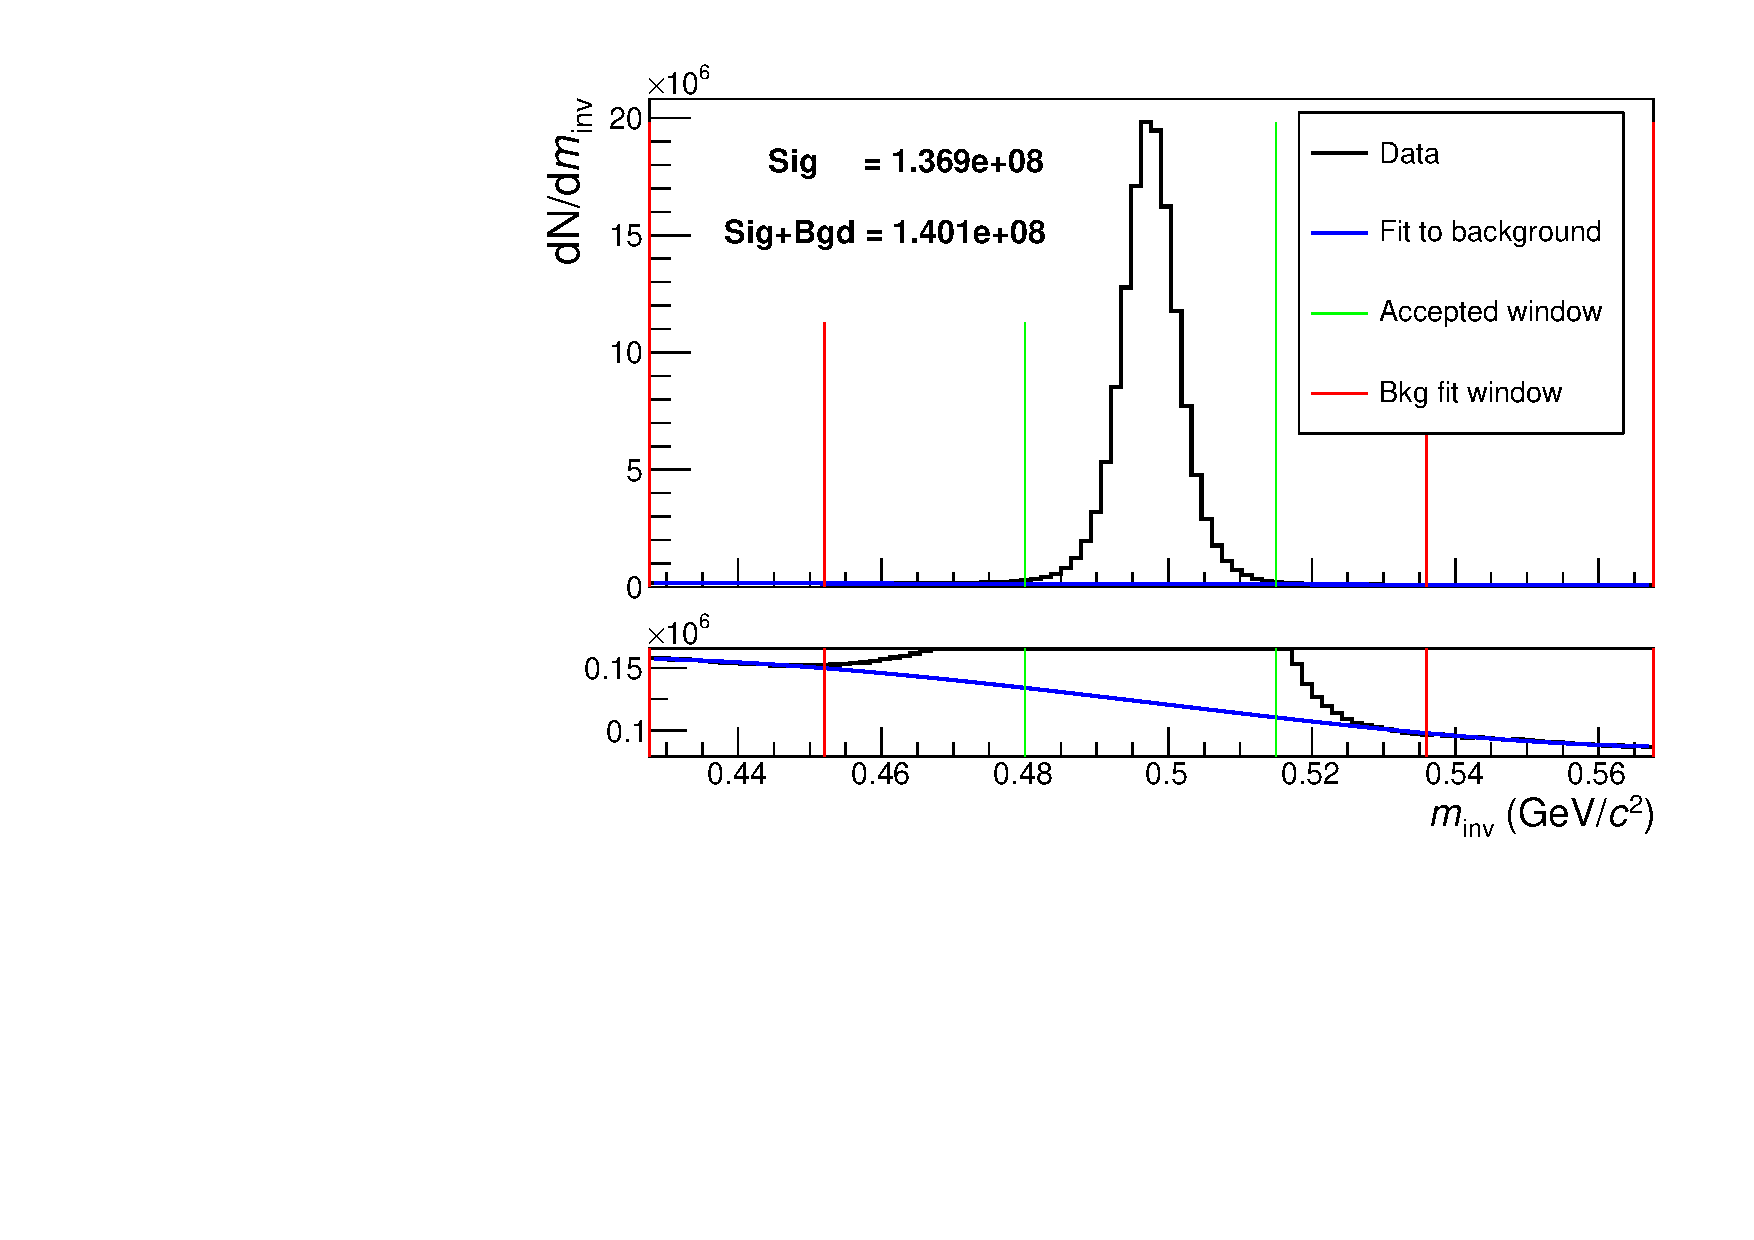
\includegraphics[width=0.49\linewidth]{/home/jesse/Analysis/FemtoAnalysis/LamKPublication/Figures/PDF/K0Purity_LamK0.pdf}}
   %%----overall caption----
-  \caption{Invariant mass (\minv) distribution of p$\pi^{+}$ pairs showing the \Lam peak \ref{fig:Purity:a}, and of $\pi^{+}\pi^{-}$ pairs showing the \Ks peak \ref{fig:Purity:b}, for \Vz candidates.  The bottom panels are zoomed to show the background with fit.  The vertical green lines represent the \minv cuts used in the analyses, the red vertical lines delineate the region over which the background was fit, and the blue line shows the background fit.}  
+  \caption{
+  (Color online) Invariant mass (\minv) distribution of p$\pi^{+}$ pairs showing the \Lam peak \ref{fig:Purity:a}, and of $\pi^{+}\pi^{-}$ pairs showing the \Ks peak \ref{fig:Purity:b}, for \Vz candidates.  
+  The bottom panels are zoomed to show the background with fit.  
+  The vertical dashed lines represent the \minv cuts used in the analyses, the vertical dotted lines delineate the region over which the background was fit, and the dash-dotted line shows the background fit.
+  }  
   \label{fig:Purity}
 \end{figure}
 
@@ -501,8 +510,6 @@
 \end{equation}
 where $\mathbf{k}^{*}$ is the relative momentum of the pair (defined as $\mathbf{k}^{*} = \frac{1}{2}|\mathbf{p}_{1}^{*}-\mathbf{p}_{2}^{*}|$, where $\mathbf{p}_{1}^{*}$ and $\mathbf{p}_{2}^{*}$ are the momenta of the two particles) in the pair rest frame (PRF), $\mathbf{r}^{*}$ is the relative separation in the same frame, $\mathbf{P}$ is the total pair momentum, $S_{\mathbf{P}}(\mathbf{r^{*}})$ is the pair source distribution, and $\Psi_{\mathbf{k^{*}}}(\mathbf{r^{*}})$ is the two-particle wave-function.
 Within the $|\Psi|^{2}$ term is contained the particle interaction information, and therefore the scattering parameters.
\sout{\color{red}{Equation \ref{eqn:KooninPrattEqn} reveals the limitations of femtoscopy; at best, it can probe the distribution of relative positions of particles with identical velocities and total momentum $\mathbf{P}$ as they move in an asymptotic state \cite{Lisa:2005dd}.}}
\sout{\color{red}{Therefore, the entire size of the source is not measured, but rather the ``regions of homogeneity'' \cite{Akkelin:1995gh}.}}
 

 In practice, $A(k^{*})$ is constructed by binning in \kstar pairs from the same event.
\sout{\color{red}{Typically, $B(k^{*})$ is obtained by forming mixed-event pairs \cite{Kopylov:1974th}, i.e. particles from a given event are paired with particles from $\rm N_{mix}$ other events, and these pairs are then binned in \kstar.}}
\sout{\color{red}{Other techniques exist; most notably, one may use same-event pairs after rotating one particle in the pair by 180$^\circ$ in the transverse plane (see Sec. \ref{NonFlatBackground} and App. \ref{App:StavMethod} for more details).}}
\sout{\color{red}{For this analysis, the typical mixed-event method is utilized, and each event is mixed with $\rm N_{mix} =$ 5 others for the reference distribution construction.}}
\underline{\color{blue}{Typically, $B(k^{*})$ is obtained using mixed-event pairs \cite{Kopylov:1974th}, i.e. particles from a given event are paired with those from another event.}}
\underline{\color{blue}{Other techniques exist; most notably, one may use same-event pairs after rotating one particle in the pair by 180$^\circ$ in the transverse plane (see Sec.\ \ref{NonFlatBackground} and App.\ \ref{App:StavMethod} for more details).}}
\underline{\color{blue}{For this analysis, the typical mixed-event method is utilized, and each event is mixed with five others for the reference distribution construction.
 In order to mix only similar events, events are binned both in primary vertex location (2 cm bin width) and in centrality (5\% bin width), and only events within a given bin are mixed; i.e. only events of like centrality and of like primary vertex location are mixed.}}
\sout{\color{red}{After the event binning, a vertex correction is applied to each event, in which the primary vertex position is subtracted from the TPC track positions for each particle in the event.}}
\sout{\color{red}{Subsequently, the tracks in an event are all measured relative to the event vertex, instead of the center of the TPC.}}
\sout{\color{red}{This effectively gives each event the same primary vertex position, which is important for the implementation of the average separation cut in mixed-event pairs.}}
 
 This analysis presents correlation functions for three centrality bins (0--10\%, 10--30\%, and 30--50\%), and is pair transverse momentum ($k_{\mathrm{T}} = \frac{1}{2}|\mathbf{p}_{\mathrm{T,1}}+\mathbf{p}_{\mathrm{T,2}}|$) integrated (i.e. not binned in $k_{\mathrm{T}}$) due to limited statistics.
\sout{\color{red}{The $k_{\mathrm{T}}$-dependence of the three \LamK combinations should be the same, so an integrated analysis is acceptable.}}
\underline{\color{blue}{The $k_{\mathrm{T}}$-dependence of the three \LamK combinations is comparable, so an integrated analysis is acceptable.}}
 The correlation functions are constructed separately for the two magnetic field configurations ($++$ and $--$).
 These are kept separate during the fitting process, and are combined using a weighted average when plotting, where the weight is the number of numerator pairs in the normalization range.
 
@@ -533,23 +537,17 @@
 
 
 In the absence of the Coulomb interaction, the correlation function can be described analytically with a model derived by Lednick\'y and Lyuboshitz \cite{Lednicky:82}.
\sout{\color{red}{Within the model, the (non-symmetrized) two-particle wave function is expressed as a superposition of a plane wave and diverging spherical wave:}}
-\begin{equation}
-\begin{aligned}
-\Psi^{S}(\mathbf{k}^{*}, \mathbf{r}^{*}) = e^{-i\mathbf{k}^{*} \cdot \mathbf{r}^{*}} + f^{S}(k^{*})\frac{e^{ik^{*}r^{*}}}{r^{*}}
-\end{aligned}  
-\label{eqn:NonSymmPsi}
-\end{equation}
-In the effective range approximation, the complex s-wave scattering amplitude, $f^{S}(k^{*})$, with $S$ denoting the total spin of the particular pair, is of the form
+Within the model, the (non-symmetrized) two-particle wave function is expressed as a superposition of a plane wave and diverging spherical wave, and the complex scattering amplitude, $f^{S}(k^{*})$, is evaluated via the effective range approximation
 \begin{equation}
 \begin{aligned}
 f^{S}(k^{*}) = \left( \frac{1}{f^{S}_{0}} + \frac{1}{2}d^{S}_{0}k^{*2} - ik^{*} \right)^{-1}
 \end{aligned}
 \label{eqn:ScatteringParam}
 \end{equation}
\sout{\color{red}{where $f^{S}_{0}$ is the complex s-wave scattering length, and $d^{S}_{0}$ is the effective range of the interaction.}}
\underline{\color{blue}{where $f^{S}_{0}$ is the complex s-wave scattering length, $d^{S}_{0}$ is the effective range of the interaction, and $S$ denotes the total spin of the particular pair.}}
\underline{\color{blue}{The sign convention is such that a positive real component of the scattering length, $\Re f_{0}$, represents an attractive interaction, while a negative $\Re f_{0}$ represents a repulsion.}}
 A spherically symmetric Gaussian distribution with radius $R_{\mathrm{inv}}$  is assumed for the pair emission source in the PRF.
\sout{\color{red}{With these assumptions, utilizing the Koonin-Pratt equation (Eq. \ref{eqn:KooninPrattEqn}), the correlation function for non-identical particle pairs with at least one uncharged member is given by \cite{Lednicky:82}}}
\underline{\color{blue}{With these assumptions, utilizing the Koonin-Pratt equation (Eq.\ \ref{eqn:KooninPrattEqn}), the correlation function for non-identical particle pairs with at least one uncharged member is given by \cite{Lednicky:82}}}
 
 \begin{equation}
 \begin{aligned}
@@ -558,43 +556,36 @@
 \label{eqn:LednickyEqn}
 \end{equation}
 
\sout{\color{red}{where $\Re f^{S}(k^{*})$ and $\Im f^{S}(k^{*})$ denote the real and imaginary parts of the complex scattering length, respectively, and $F_{1}$ and $F_{2}$ are the analytic functions}}
-\begin{equation}
-F_{1}(z) = \int_{0}^{z} \frac{e^{x^{2}-z^{2}}}{z}dx; \qquad
-F_{2}(z) = \frac{1-e^{-z^{2}}}{z}.
-\label{eqn:CFSI2}
-\end{equation}
-
\underline{\color{blue}{where $\Re f^{S}(k^{*})$ and $\Im f^{S}(k^{*})$ denote the real and imaginary parts of the complex scattering length, respectively, and $F_{1}$ and $F_{2}$ are the analytic functions.}}
 The weight factor, $\rho_{S}$ is the normalized emission probability for a state of total spin $S$; in the assumed case of unpolarized emission, $\rho_{S} = (2S+1)/[(2j_{1}+1)(2j_{2}+1)]$, where $j_{1,2}$ are the spins of the particles in the pair.
\sout{\color{red}{The \Lam hyperon is spin-1/2 and K mesons are spin-0, so the \LamK system only has one possible total spin state $S$, and therefore $C(k^{*})$ in Eq. \ref{eqn:LednickyEqn} has only a single term.}}
\underline{\color{blue}{The \Lam hyperon is spin-1/2 and K mesons are spin-0, so the \LamK system only has one possible total spin state $S$, and therefore $C(k^{*})$ in Eq.\ \ref{eqn:LednickyEqn} has only a single term.}}
 In the following, the $S$ superscript is dropped from all scattering parameters.
 
 \subsection{Residual Correlations}
 \label{ResidualCorrelations}
 
 The purpose of this analysis is study the interaction and scale of the emitting source of the primary \LamK pairs.
\sout{\color{red}{However, in practice, obtaining a pure sample of primary \LamK pairs is impossible to achieve; some of the selected particles originate as decay products from other resonances, and some of the final pairs contain a misidentified member.}}
\underline{\color{blue}{However, in practice some of the selected particles originate as decay products from other resonances, and some of the final pairs contain a misidentified member.}}
 In both cases, these contribute to the finally observed correlation function, and obscure its relation to the primary \LamK system.
\underline{\color{blue}{The contributions from fake pairs, which contain at least one misidentified member, are assumed to average to unity, in which case they simply attenuate the femtoscopic signal.}}
 Those pairs whose members originate as daughters from resonances carry information about the parent system.
 In effect, the correlation between the parents will be visible, although smeared out, in the daughters' signal.
 This is termed a residual correlation resulting from feed-down.  
\sout{\color{red}{For this analysis, a portion of the selected \Lam hyperons decay from $\Sigma^{0}$, $\Xi^{0}$, $\Xi^{-}$ and $\Sigma^{*(+,-,0)}(1385)$ parents, and some of the K mesons decay from K$^{*(+,-,0)}(892)$ parents.}}
\sout{\color{red}{The contribution from fake pairs, which contain a misidentified member, is assumed to average to unity, in which case it leads to an attenuation of the femtoscopic signal.}}
-
-
-The finally measured correlation function is a combination of the genuine \LamK correlation with contributions from residual feed-down and misidentified particles
-\begin{eqnarray}
+As described in the following, the main sources of residual correlations in the \LamK systems result from \Lam hyperons which have decayed from $\Sigma^{0}$, $\Xi^{0}$, and $\Xi^{-}$ parents.
+
+The finally measured correlation function is a combination of the genuine \LamK correlation with contributions from resonances and impurities \cite{Kisiel:2014mma}
+\begin{equation}
+\begin{aligned}
 \label{eqn:CfwRes} 
- C_{\mathrm{measured}}(k^{*}_{\Lambda\mathrm{K}}) &=& 1 + \lambda'_{\Lambda\mathrm{K}}[C_{\Lambda\mathrm{K}}(k^{*}_{\Lambda\mathrm{K}}) - 1] + \sum\limits_{i,j}  \lambda'_{ij}[C_{ij}(k^{*}_{\Lambda\mathrm{K}})-1] \\
- \lambda_{ij}' &=& \lambda_{\mathrm{Fit}}\lambda_{ij} \notag \\
- \sum\limits_{i,j}\lambda_{ij}' &=&  \lambda_{\mathrm{Fit}}\sum\limits_{i,j}\lambda_{ij} = \lambda_{\mathrm{Fit}} \notag
-\end{eqnarray}
-where the \LamK term represents the genuine \LamK correlation, and the $ij$ terms denote the contributions from residual feed-down and possible impurities.
-More specifically, $C_{ij}(k^{*}_{\Lambda\mathrm{K}})$ is the correlation function between parents of particle species $i$ and $j$, expressed in terms of the relative momentum of the observed daughter \LamK pairs.  
-The $\lambda_{ij}$ parameters serve as weights dictating the relative strength of the parent contribution to the daughter pair, and are normalized to unity (i.e. $\sum_{ij} \lambda_{ij} = 1$, where $ij$ includes also the primary \LamK component).
-The individual $\lambda_{ij}$ are fixed (and whose values can be found in Table \ref{tab:LambdaValues_3Res}), but the parameter $\lambda_{\mathrm{Fit}}$ is left free.
-The $\lambda_{\mathrm{Fit}}$ parameter serves as an common factor shared by all contributors, as shown in Eq. \ref{eqn:CfwRes}.
-
+ C_{\mathrm{measured}}(k^{*}_{\Lambda\mathrm{K}}) &= 1 + \lambda'_{\Lambda\mathrm{K}}[C_{\Lambda\mathrm{K}}(k^{*}_{\Lambda\mathrm{K}}) - 1] + \sum\limits_{ij}  \lambda'_{ij}[C_{ij}(k^{*}_{\Lambda\mathrm{K}})-1] \\
+ \lambda_{ij}' &= \lambda_{\mathrm{Fit}}\lambda_{ij} \\
+ \sum\limits_{ij}\lambda_{ij}' &=  \lambda_{\mathrm{Fit}}\sum\limits_{ij}\lambda_{ij} = \lambda_{\mathrm{Fit}}
+\end{aligned} 
+\end{equation}
+where the \LamK term represents the genuine \LamK correlation, and the $ij$ terms denote the contributions from residual feed-down and impurities.
+More specifically, $C_{ij}(k^{*}_{\Lambda\mathrm{K}})$ is the correlation function of the parent system expressed in terms of the relative momentum of the daughter \LamK pair.  
+The $\lambda_{ij}$ parameters serve as weights dictating the relative strength of each component's contribution to the observed signal, and are normalized to unity (i.e. $\sum_{ij} \lambda_{ij} = 1$, where $ij$ includes also the primary \LamK component).
+The individual $\lambda_{ij}$ are fixed (and whose values can be found in Table \ref{tab:LambdaValues_3Res}), but the parameter $\lambda_{\mathrm{Fit}}$ in Eq.\ \ref{eqn:CfwRes} is left free.
 
 \begin{table}[htbp]
  \centering
@@ -606,9 +597,9 @@
   \textbf{Source} & \textbf{$\lambda$ value} & \textbf{Source} & \textbf{$\lambda$ value} & \textbf{Source} & \textbf{$\lambda$ value} & \textbf{Source} & \textbf{$\lambda$ value} \\
   \hlineB{3.0}
   Primary & 0.527 & Primary & 0.526 & Primary & 0.526 & Primary & 0.527 \\
-  $\Sigma^{0}$K$^{+}$ & 0.111 & $\bar{\Sigma}^{0}$K$^{-}$ & 0.110 & $\Sigma^{0}$K$^{-}$ & 0.110 & $\bar{\Sigma}^{0}$K$^{+}$ & 0.111 \\  
-  $\Xi^{0}$K$^{+}$ & 0.039 & $\bar{\Xi}^{0}$K$^{-}$ & 0.035 & $\Xi^{0}$K$^{-}$ & 0.038 & $\bar{\Xi}^{0}$K$^{+}$ & 0.036 \\  
-  $\Xi^{-}$K$^{+}$ & 0.050 & $\bar{\Xi}^{+}$K$^{-}$ & 0.046 & $\Xi^{-}$K$^{-}$ & 0.050 & $\bar{\Xi}^{+}$K$^{+}$ & 0.046 \\  
+  $\Sigma^{0}$K$^{+}$ & 0.111 & $\overline{\Sigma}^{0}$K$^{-}$ & 0.110 & $\Sigma^{0}$K$^{-}$ & 0.110 & $\overline{\Sigma}^{0}$K$^{+}$ & 0.111 \\  
+  $\Xi^{0}$K$^{+}$ & 0.039 & $\overline{\Xi}^{0}$K$^{-}$ & 0.035 & $\Xi^{0}$K$^{-}$ & 0.038 & $\overline{\Xi}^{0}$K$^{+}$ & 0.036 \\  
+  $\Xi^{-}$K$^{+}$ & 0.050 & $\overline{\Xi}^{+}$K$^{-}$ & 0.046 & $\Xi^{-}$K$^{-}$ & 0.050 & $\overline{\Xi}^{+}$K$^{+}$ & 0.046 \\  
   Other & 0.226 & Other & 0.235 & Other & 0.228 & Other & 0.233 \\  
   Fakes & 0.048 & Fakes & 0.048 & Fakes & 0.048 & Fakes & 0.048 \\
   \hlineB{3.0}
@@ -620,9 +611,9 @@
   \multicolumn{2}{c|}{} & \textbf{Pair System} & \textbf{$\lambda$ value} & \textbf{Pair System} & \multicolumn{1}{c|}{\textbf{$\lambda$ value}} & \multicolumn{2}{c}{} \\
   \clineB{3-6}{3.0}
   \multicolumn{2}{c|}{} & Primary & 0.543 & Primary & \multicolumn{1}{c|}{0.544} & \multicolumn{2}{c}{} \\  
-  \multicolumn{2}{c|}{} & $\Sigma^{0}$K$^{0}_{\mathrm{S}}$ & 0.120 & $\bar{\Sigma}^{0}$K$^{0}_{\mathrm{S}}$ & \multicolumn{1}{c|}{0.120} & \multicolumn{2}{c}{} \\  
-  \multicolumn{2}{c|}{} & $\Xi^{0}$K$^{0}_{\mathrm{S}}$ & 0.042 & $\bar{\Xi}^{0}$K$^{0}_{\mathrm{S}}$ & \multicolumn{1}{c|}{0.039} & \multicolumn{2}{c}{} \\  
-  \multicolumn{2}{c|}{} & $\Xi^{-}$K$^{0}_{\mathrm{S}}$ & 0.054 & $\bar{\Xi}^{+}$K$^{0}_{\mathrm{S}}$ & \multicolumn{1}{c|}{0.050} & \multicolumn{2}{c}{} \\  
+  \multicolumn{2}{c|}{} & $\Sigma^{0}$K$^{0}_{\mathrm{S}}$ & 0.120 & $\overline{\Sigma}^{0}$K$^{0}_{\mathrm{S}}$ & \multicolumn{1}{c|}{0.120} & \multicolumn{2}{c}{} \\  
+  \multicolumn{2}{c|}{} & $\Xi^{0}$K$^{0}_{\mathrm{S}}$ & 0.042 & $\overline{\Xi}^{0}$K$^{0}_{\mathrm{S}}$ & \multicolumn{1}{c|}{0.039} & \multicolumn{2}{c}{} \\  
+  \multicolumn{2}{c|}{} & $\Xi^{-}$K$^{0}_{\mathrm{S}}$ & 0.054 & $\overline{\Xi}^{+}$K$^{0}_{\mathrm{S}}$ & \multicolumn{1}{c|}{0.050} & \multicolumn{2}{c}{} \\  
   \multicolumn{2}{c|}{} & Other & 0.194 & Other & \multicolumn{1}{c|}{0.199} & \multicolumn{2}{c}{} \\  
   \multicolumn{2}{c|}{} & Fakes & 0.048 & Fakes & \multicolumn{1}{c|}{0.048} & \multicolumn{2}{c}{} \\
   \clineB{3-6}{3.0} 
@@ -632,54 +623,54 @@
 \end{table}
 
 
\sout{\color{red}{In order to obtain the parent correlation function expressed in the relative momentum of the daughter pair, one must use a transform matrix.}}
\sout{\color{red}{The transform matrix describes the decay kinematics of the parent system into the daughter, and maps the \kstar of the parent pair onto that of the daughter.}}
\sout{\color{red}{Using this matrix, the transformed residual correlation function can be obtained:}}
+To obtain the parent correlation function expressed in the relative momentum of the daughter pair, a transform matrix is utilized
 \begin{equation}
   C_{ij}(k^{*}_{\Lambda\mathrm{K}}) \equiv \frac{\sum\limits_{k^{*}_{ij}} C_{ij}\left(k^{*}_{ij}\right) T\left(k^{*}_{ij},k^{*}_{\Lambda\mathrm{K}}\right)}{\sum\limits_{k^{*}_{ij}} T\left(k^{*}_{ij},k^{*}_{\Lambda\mathrm{K}}\right)}
 \label{eqn:ResidualsTransform}
 \end{equation}
\sout{\color{red}{The transform matrix is generated with the THERMINATOR 2 \cite{Chojnacki:2011hb} simulation. }}
\sout{\color{red}{It is formed for a given parent pair, $ij$, by taking all \LamK pairs originating from $ij$, calculating the relative momentum of the parents ($k^{*}_{ij}$) and daughters ($k^{*}_{\Lambda\mathrm{K}}$), and filling a two-dimensional histogram with the values. }}
\sout{\color{red}{The transform matrix is essentially an unnormalized probability distribution mapping the \kstar of the parent pair to that of the daughter pair when one or both parents decay.}}
- 
\sout{\color{red}{As previously stated, the $\lambda$ parameters dictate the strength of the parent contribution to the daughter pair.  }}
-Therefore, the $\lambda$ parameter for parent system AB can be estimated as the total number of $\Lambda$K pairs in our experimental sample originating from AB (N$_{AB}$) divided by the total number of $\Lambda$K pairs (N$_{Total}$):
-\begin{equation}
-\lambda_{AB} = \frac{N_{AB}}{N_{Total}}
-\end{equation}
-The number of \LamK pairs originating from each source involves not only the raw yields for each, but also the corresponding experimental reconstruction efficiencies.
+where $T(k^{*}_{ij},k^{*}_{\Lambda\mathrm{K}})$ is the transform matrix, which is generated with the THERMINATOR 2 \cite{Chojnacki:2011hb} simulation. 
+The transform matrix describes the decay kinematics of the parent system into the daughter, and is essentially an unnormalized probability distribution mapping the \kstar of the parent pair to that of the daughter pair when one or both parents decay (see Ref.\ \cite{Kisiel:2014mma} for more details).
+
+
+In practice, the contribution of a parent system (e.g. $\Sigma^{0}$\KchP) to the daughter correlation function (e.g. \LamKchP) is determined by modeling the parent system's correlation function and running it through the appropriate transform matrix.
+Since the interactions between these particles are not known, all residual pairs are assumed to have the same source size as the daughter pair.
+Furthermore, Coulomb-neutral residual pairs are assumed to share the same scattering parameters as the daughter pair.
+When modeling \XiKpm residual correlations, the experimental \XiKpm data is used. 
+Consistent results are found when modeling the \XiKpm system, in which the the strong interaction is assumed to be negligible, and the parent correlation is generated assuming a Coulomb-only scenario (see Appendix \ref{App:CoulombFitter} for more details).
+This approximation is well justified here as a Coulomb-only description of the system describes, reasonably well, the broad features of the correlation.   
+
+The $\lambda_{ij}$ parameters dictate the relative strength of each contribution to the correlation function, and can be estimated using the THERMINATOR 2 and HIJING simulations.
+More specifically, a $\lambda_{ij}$ parameter is estimated as the total number of \LamK pairs in the experimental sample originating from $ij$ ($N_{ij}$) divided by the total number of \LamK pairs ($N_{\mathrm{Total}}$).
+The number of detected \LamK pairs involves both the raw yields and the reconstruction efficiencies.
 The reconstruction efficiencies ($RE_{ij}$) are estimated with MC HIJING data, which has been run through GEANT to simulate the detector response.
 HIJING events are generated from a superposition of PYTHIA p-p collisions, and lack the strangeness saturation of a fully thermalized medium.
 As a result, HIJING is unreliable in providing the yields needed for this analysis, and, instead, the yields are estimated with the THERMINATOR 2 simulation ($N_{ij}^{\scaleto{THERM}{3pt}}$).
-The $\lambda$ parameters are then estimated as
-\begin{equation}
-\lambda_{AB} = \frac{N_{AB}}{N_{Total}} = \frac{N_{AB}^{\scaleto{THERM}{3pt}}RE_{AB}^{\scaleto{HIJING}{3pt}}}{\sum\limits_{ij} N_{ij}^{\scaleto{THERM}{3pt}}RE_{ij}^{\scaleto{HIJING}{3pt}}}
-\end{equation}
+The number of \LamK pairs is then estimated as the product of the yield with the reconstruction efficiency, $N_{ij} = N_{ij}^{\scaleto{THERM}{3pt}}RE_{ij}^{\scaleto{HIJING}{3pt}}$.
+
+
 
 Femtoscopic analyses are sensitive to the pair emission structure at kinetic freeze-out.
 Therefore, in the eyes of femtoscopy, any particle born from a resonance decay before last rescattering is seen as primary.
-For this study, a particle is considered to be primary if its parent has a proper decay length of $c\tau <$ 10 fm. 
-With this selection, residual contributions from $\Sigma^{0}$, $\Xi^{0}$, $\Xi^{-}$ must be accounted for in the fit.
-The $\lambda$ values used can be found in Table \ref{tab:LambdaValues_3Res}, which also included values for ``Other'' and ``Fakes''.  
+The THERMINATOR 2 simulation shows that, aside from primaries, the \Lam hyperons and K mesons decay from a large number of resonances ($\sim$50 \Lam parent species, and $\sim$70 K parent species), and the most significant contributing pair systems are $\Sigma^{0}$K, $\Xi^{-}$K, $\Xi^{0}$K, $\Sigma^{*+}$K, $\Sigma^{*-}$K, $\Sigma^{*0}$K, $\Lambda\mathrm{K}^{*}$, $\Sigma^{0}\mathrm{K}^{*}$, $\Xi^{-}\mathrm{K}^{*}$, and $\Xi^{0}\mathrm{K}^{*}$.
+However, the simulation does not include a hadronic rescattering phase, and not all of the aforementioned pair systems will survive until kinetic freeze-out.
+The systems resulting from electromagnetic or weak decays ($\Sigma^{0}$, $\Xi^{-}$, and $\Xi^{0}$) will survive long after kinetic freeze-out, and will contribute residual signals to the \LamK correlation functions.
+The majority of the remaining contributors decay via the strong interaction with mean proper lifetimes less than a few fm/$c$, and whose daughters should always be considered primary.
+The mean proper lifetime of the parent is used to judge whether or not the daughter is treated as primary.
+A decay product is considered primary if its parent has a mean proper lifetime $\tau$ satisfying $c\tau <$ 10 fm.
+Changing $c\tau$ only moderately affects the $\lambda_{ij}$ parameters, and the effect is included the estimation of the systematic uncertainties.
+In order for a pair to be considered primary, both particles in the pair must be considered primary. 
+If either parent has $\tau > \tau_{\mathrm{max}}$, the daughter pair contributes to the ``Other" category when calculating $\lambda$ parameters.
+For this hodgepodge of pair systems, all with different two-particle interactions and single-particle source distributions, we assume the net correlation effect averages to unity.
+
+
+Residual contributions from $\Sigma^{0}$, $\Xi^{0}$, $\Xi^{-}$ are accounted for in the fit.
+The $\lambda_{ij}$ values used can be found in Table \ref{tab:LambdaValues_3Res}, which also included values for ``Other'' and ``Fakes''.  
 The ``Other'' category contains pairs which are not considered primary, and which do not originate from the residual contributors accounted for in the fit.  
 The ``Fakes'' category represents pairs that are mistakenly identified as \LamK.  
-To estimate this $\lambda_{\mathrm{Fakes}}$ value, the number of fake pairs is assumed to be equal to the total number of pairs multiplied by the \Lam purity (i.e. assuming perfect purity for the kaons); or, more simply, $\lambda_{\mathrm{Fakes}}$ = 1.0 $-$ Purity(\Lam).  
-For both of these contributors (``Other'' and ``Fakes''), it is assumed that these correlations average to unity, and therefore do not contribute to the final correlation function.
-
-In practice, the contribution of a parent system (e.g. $\Sigma^{0}$\KchP) to the daughter correlation function (e.g. \LamKchP) is determined by modeling the parent system's correlation function and running it through the appropriate transform matrix.
-However, little is know about the interaction between the particles in the residual pairs of this study, and assumptions must be made.
-For this analysis, all residual pairs are assumed to have the same source size as the daughter pair.
-Furthermore, Coulomb-neutral residual pairs are assumed to share the same scattering parameters as the daughter pair.
-Therefore, for Coulomb-neutral pairs, such as $\Sigma^{0}$K, and $\Xi^{0}$K, $C_{ij}(k^{*}_{ij})$ is calculated from Eqn. \ref{eqn:LednickyEqn}, with the help of Eqn. \ref{eqn:CFSI2}; $C_{ij}(k^{*}_{\Lambda\mathrm{K}})$ is then obtained by transforming $C_{ij}(k^{*}_{ij})$ with Eq. \ref{eqn:ResidualsTransform}, using the appropriate transform matrix.  
-
-For residual pairs affected by both the strong and Coulomb interactions, things are a bit more complicated.
-This is due to the fact that, for the case of both strong and Coulomb interaction, there no longer exists a nice analytical form with which to fit.
-Generating a correlation function including both is also time consuming, as described further in Appendix \ref{App:CoulombFitter}.
-When modeling \XiKpm residual correlations, the experimental \XiKpm data is used; in this case, there is no need to make any assumptions about scattering parameters or source sizes. 
-Consist results are found when modeling the \XiKpm system, in which the the strong interaction is assumed to be negligible, and the parent correlation is generated assuming a Coulomb-only scenario (see Appendix \ref{App:CoulombFitter} for more details).
-This approximation is well justified here as a Coulomb-only description of the system describes, reasonably well, the broad features of the correlation; the strong interaction is necessary for the fine details.  
-As these correlations are run through a transform matrix, which largely flattens out and fine details, a Coulomb-only description should be sufficient.   
+To estimate the $\lambda_{\mathrm{Fakes}}$ value, the number of fake pairs is assumed to be equal to the total number of simulated pairs multiplied by $(1-PP_{\Lambda\mathrm{K}})/PP_{\Lambda\mathrm{K}}$, where $PP_{\Lambda\mathrm{K}}$ is the \LamK pair purity, estimated as the product of the two single-particle purities ($PP_{\Lambda\mathrm{K}} = P_{\Lambda}P_{\mathrm{K}}$).
+More simply, this amounts to $\lambda_{\mathrm{Fakes}} = 1.0-PP_{\Lambda\mathrm{K}}$.
+The correlations in both of these categories (``Other'' and ``Fakes'') are assumed to average to unity, and pairs in these categories therefore only contribute by attenuating the signal. 
+
 
 
 \subsection{Momentum Resolution Corrections}
@@ -688,7 +679,6 @@
 Finite track momentum resolution causes the reconstructed momentum of a particle to smear around the true value.
 This, of course, also holds true for \Vz particles.
 The effect is propagated up to the pairs of interest, which causes the reconstructed relative momentum (\krec) to differ from the true momentum (\ktrue).
-Smearing of the momentum typically will result in a suppression and broadening of the signal.
 The effects of finite momentum resolution are accounted for through the use of a response matrix generated with MC HIJING data.
 With this approach, the resolution correction is applied on-the-fly during the fitting process by propagating the theoretical (fit) correlation function through the response matrix, according to
 \begin{equation}
@@ -696,51 +686,43 @@
 \label{eqn:MomResCorrection}
 \end{equation}
 where $M_{k^{*}_{\mathrm{Rec}},k^{*}_{\mathrm{True}}}$ is the response matrix, $C_{\mathrm{fit}}(k^{*}_{\mathrm{True}})$ is the fit binned in \ktrue, and the denominator normalizes the result.
-Equation \ref{eqn:MomResCorrection} describes that, for a given \krec bin, the observed value of $C(k^{*}_{\mathrm{Rec}})$ is a weighted average of all $C(k^{*}_{\mathrm{True}})$ values, where the weights are the normalized number of counts in the [\krec, \ktrue] bin.
+Equation \ref{eqn:MomResCorrection} describes that, for a given \krec bin, the observed value of $C(k^{*}_{\mathrm{Rec}})$ is a weighted average of all $C(k^{*}_{\mathrm{True}})$ values, where the weights are the normalized number of counts in the \mbox{$[k^{*}_{\mathrm{Rec}}, k^{*}_{\mathrm{True}}]$} bin.
 
 
 
 \subsection{Non-Femtoscopic Background}
 \label{NonFlatBackground}
 
-A significant non-femtoscopic, non-flat, background is observed in all of the studied \LamK correlations at large \kstar.  
-This background increases with decreasing centrality, is the same amongst all \LamKpm pairs, and is more pronounced in the \LamKs system.
-This difference in \LamKpm and \LamKs backgrounds is due mainly to the difference in kinematic cuts, not due to any interesting physics.  
-
-It is suggested that this background effect is due primarily to particle collimation associated with elliptic flow \cite{Kisiel:2017}.  
-More specifically, these backgrounds result from mixing events with unlike event-plane angles ($\Psi_{\textrm{EP}}$).  
-As explained in \cite{Kisiel:2017}, when elliptic flow is present, all particles are more likely to be emitted in a specific direction (in-plane), as opposed to a perpendicular direction.  
-Therefore, the difference in momenta for pairs of particles tends to be smaller, compared to the case of no flow.  
-In the case of mixed-event pairs, the two events used do not share an event-plane, and therefore there is no collimation effect in the pairs from flow.  
-As a result, pairs with larger momentum are more likely when mixed-events are used (in the denominator of the correlation function), causing the correlation function to dip below unity.  
-This same reasoning suggests that the background should lead to an enhancement at low-\kstar. 
-An attempt was made to decrease this background through the binning of events in $\Psi_{\mathrm{EP}}$, but only a small reduction in the signal was achieved due to the limited event-plane resolution.
-
-THERMINATOR 2 simulation has been shown to reproduce the background features in a $\pi$K analysis \cite{Kisiel:2017}.  
-After issuing each simulated event a random $\Psi_{\mathrm{EP}}$, THERMINATOR 2 did an exceptional job of describing the \LamK data.  
-Furthermore, the simulation showed the non-femtoscopic background affects the correlation function as a separable scale factor.
-Figure \ref{fig:BgdswTHERM} shows the THERMINATOR 2 simulation (gold) together with experimental data (red, blue, or black).  
-The figure also shows a 6$^{th}$-order polynomial fit to the simulation (gold), as well as the fit polynomial scaled to match the data (red, blue, black).
+A significant non-femtoscopic background is observed in all of the studied \LamK correlations which increases with decreasing centrality, is the same amongst all \LamKpm pairs, and is more pronounced in the \LamKs system (the difference in \LamKpm and \LamKs backgrounds is due mainly to a difference in kinematic cuts).  
+The background is due primarily to particle collimation associated with elliptic flow, and results from mixing events with unlike event-plane angles\footnote[1]
+{
+An attempt was made to decrease the background by binning events in $\Psi_{\mathrm{EP}}$, but only a small reduction in the signal was achieved due to the limited event-plane resolution.
+}\cite{Kisiel:2017}.
+The effect produces to the observed suppression at intermediate-\kstar, and should also lead to an enhancement at low-\kstar,
+The behavior of the non-femtoscopic background is needed in the low-\kstar signal region, but a clean view of it is only possible outside of such a region.
+
+The THERMINATOR 2 simulation has been shown to reproduce the background features in a $\pi$K analysis \cite{Kisiel:2017}. 
+The simulation does not include any final-state effects, but they can be introduced by weighting the numerator pairs with the modulus squared of the appropriate two-particle wave-function when building the signal distributions. 
+For the present purpose, only the behavior of the non-femtoscopic background is desired, and unit weights are used.
+Figure \ref{fig:BgdswTHERM} shows the THERMINATOR 2 simulation (open triangles) together with experimental data (closed circles).  
+The figure also shows a 6$^{\mathrm{th}}$-order polynomial fit to the simulation (dashed curves), as well as the fit polynomial scaled to match the data (solid curves).
 
 The description by THERMINATOR 2 of the non-femtoscopic backgrounds in the \LamKpm systems is remarkable, and can be used in a quantitative fashion to help fit the data.
 More specifically, the non-femtoscopic backgrounds were modeled by (6$^{\mathrm{th}}$-order) polynomial fits to THERMINATOR 2 simulation for the \LamKpm analyses; one polynomial for each centrality class.
-The form of each polynomial was set before use with the experimental data, by fitting to the THERMINATOR 2 simulation, shown in Fig. \ref{fig:BgdswTHERM}.
-At the time of the fit, the polynomial used to correct each correlation function could only be adjust by a simple scale factor to best match the data.
-The description of the \LamKs is good at a qualitative level, but not quantitatively good enough to be utilized in the fit.
-As such, a linear form is used to model the background in the \LamKs system.
-The background for each correlation function was fixed before use in the signal region by fitting a linear form to the region $0.6 < k^{*} < 0.9$ GeV/$c$.
+The form of each polynomial is set before use with the experimental data, by fitting to the THERMINATOR 2 simulation, shown in Fig.\ \ref{fig:BgdswTHERM}.
+The extracted polynomial is adjusted to best describe the data by introducing a scale factor and a vertical shift, both of which are determined by fitting to data in the region $0.32 < k^{*} < 0.80$ GeV/$c$; during the fit of the low-\kstar signal region, the background is fixed.
 In all cases, the non-femtoscopic background correction was applied as a scale factor.
 
 \begin{figure}[h]
   \centering
-  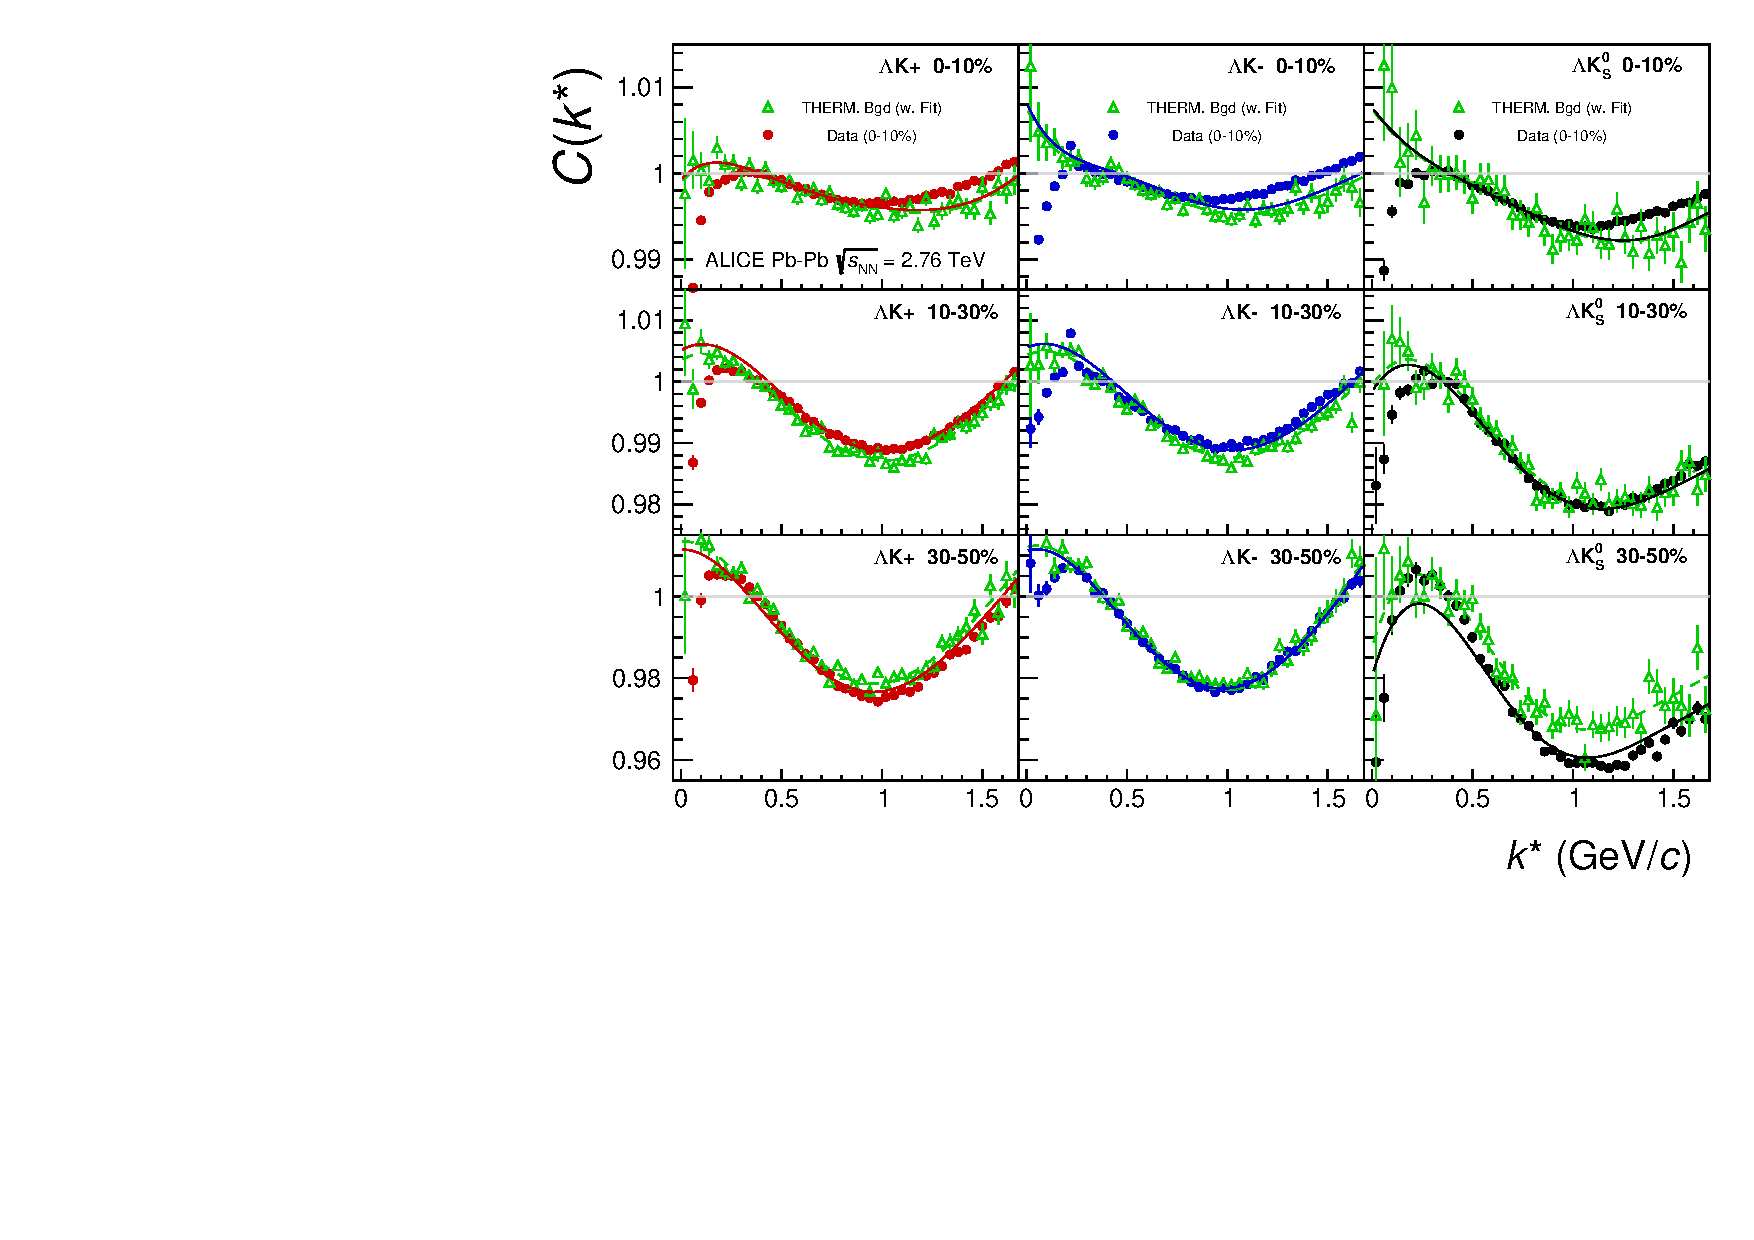
\includegraphics[width=\textwidth]{/home/jesse/Analysis/FemtoAnalysis/AnalysisNotes/5_Fitting/5.5_NonFlatBackground/Figures/BgdwFitOnly_RandomEPs_NumWeight1_PrimaryOnly_AllAnwConj_1030_3050.pdf}
+  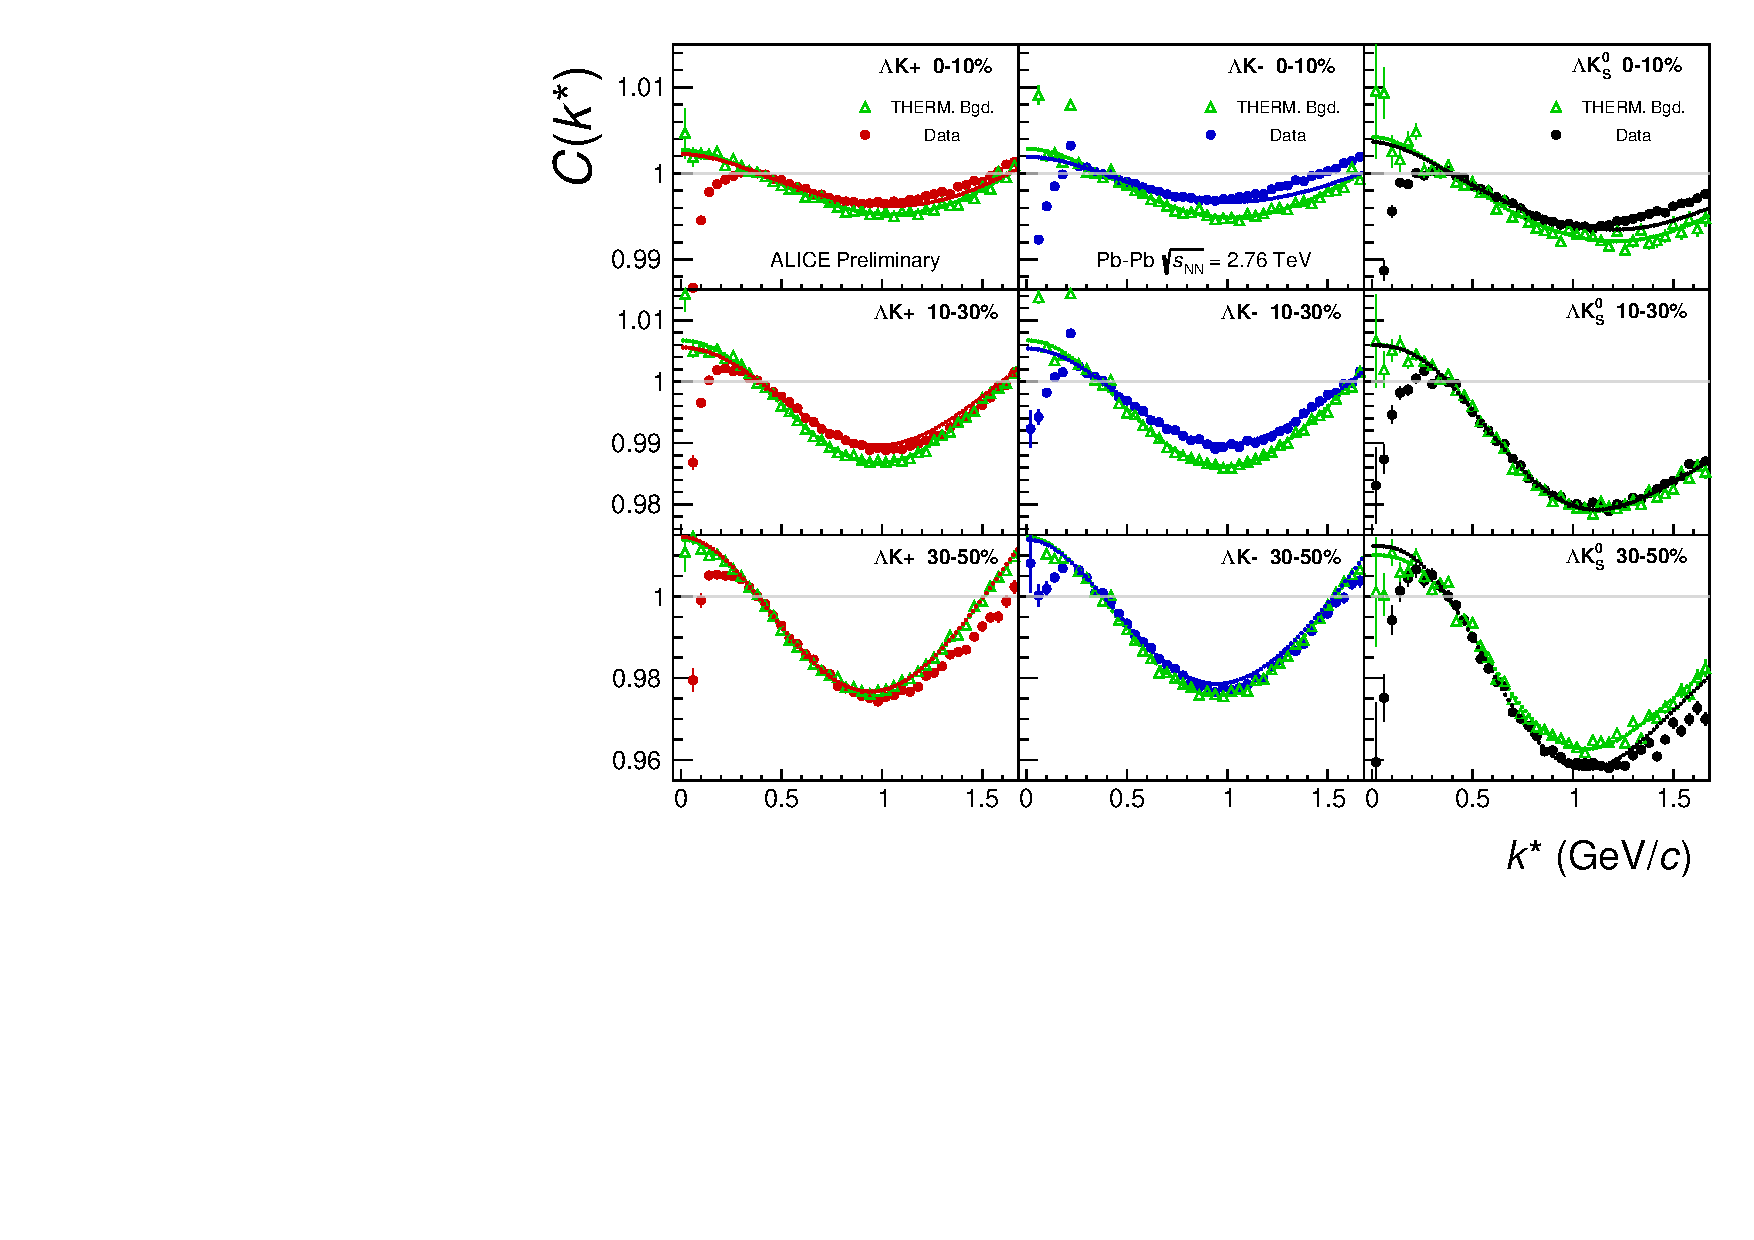
\includegraphics[width=\textwidth]{/home/jesse/Analysis/FemtoAnalysis/AnalysisNotes/5_Fitting/5.5_NonFlatBackground/Figures/BgdwFitOnly_RandomEPs_NumWeight1_Full_AllAnwConj_1030_3050.pdf}
   \caption[Backgrounds with THERMINATOR 2]
   {
-  THERMINATOR 2 simulation (gold) together with experimental data (red, blue, or black).  
+  (Color online) THERMINATOR 2 simulation (open triangles) together with experimental data (closed circles).  
   Results are shown for \LamKchP (left), \LamKchM (middle), and \LamKs (right).
-  A 6$^{th}$-order polynomial fit to the simulation is shown as a solid gold line.  
+  A $6^{\mathrm{th}}$-order polynomial fit to the simulation is shown as a dashed curve.  
   This polynomial is scaled to match the experimental data.  
-  The polynomial fit with scale factor applied is drawn in a color matching the experimental data (red, blue, black).
+  The polynomial fit with scale factor applied is drawn as a solid curve.
   }
   \label{fig:BgdswTHERM}
 \end{figure} 
@@ -750,100 +732,84 @@
 The background may be effectively reduced by forming the reference distribution ($B(k^{*})$) with the ``Stavinskiy method".
 With the Stavinskiy method, mixed-event pairs are not used for the reference distribution; instead, same-event pseudo-pairs, formed by rotating one particle in a real pair by 180$^\circ$ in the transverse plane, are used.  
 This rotation rids the pairs of any femtoscopic correlation, while maintaining correlations due to elliptic flow (and other suitably symmetric contributors).
-The effect on the \LamKchP correlation functions can be seen in the appendix, in Fig. \ref{fig:StavCfs_Correct_LamKchP}.
-
-
-\subsection{Summarized Fit Procedure}
+The effect on the \LamKchP correlation functions can be seen in the appendix, in Fig.\ \ref{fig:StavCfs_Correct_LamKchP}.
+
+
+\subsection{Summarized correlation function construction}
 \label{SummarizedFitProcedure}
 
-
-A simple $\chi^{2}$ test is inappropriate for fitting correlation functions, as the ratio two Poisson distributions does not result in a Poisson distribution.
-Instead, a log-likelihood fit function of the following form is used \cite{Lisa:2005dd}:
-
-\begin{equation}
- \chi^{2}_{PML} = -2\left[A\ln\left(\frac{C(A+B)}{A(C+1)}\right) + B\ln\left(\frac{A+B}{B(C+1)}\right)\right]
-\label{eqn:Chi2PML}
-\end{equation}
-
-where $A$ is the experimental signal distribution (numerator), $B$ is the experimental reference distribution (denominator), and $C$ is the theoretical fit correlation function.
-Therefore, Eq. \ref{eqn:Chi2PML} is used as the statistic quantifying the quality of the fit.
-The parameters of the fit are: $\lambda_{\mathrm{Fit}}$, $R$, $f_{0}$ ($\Re f_{0}$ and $\Im f_{0}$ separately), $d_{0}$, and normalization $N$.
-
+The parameters included in the generation of a correlation function are: $\lambda_{\mathrm{Fit}}$, $R$, $f_{0}$ ($\Re f_{0}$ and $\Im f_{0}$ separately), $d_{0}$, and normalization $\mathcal{N}$.
 For the fit, a given pair and its conjugate (e.g. \LamKchP and \ALamKchM) share scattering parameters ($\Re f_{0}$, $\Im f_{0}$, $d_{0}$), and the three distinct analyses (\LamKchP, \LamKchM, and \LamKs) are assumed to have scattering parameters unique from each other.
 The pair emission source for a given centrality class is assumed similar between all analyses; therefore, for each centrality, all \LamK analyses share a common radius parameter.
-For each centrality class, a single $\lambda_{\mathrm{Fit}}$ parameter (see Eq. \ref{eqn:CfwRes}) is shared amongst all.
+For each centrality class, a single $\lambda_{\mathrm{Fit}}$ parameter (see Eq.\ \ref{eqn:CfwRes}) is shared amongst all.
 Finally, each correlation function has a unique normalization parameter.
 
-All correlation functions were normalized in the range 0.32 $< k^{*} <$ 0.40 GeV/c, and fit in the range 0.0 $< k^{*} <$ 0.30 GeV/c.
+All correlation functions are normalized in the range 0.32 $< k^{*} <$ 0.40 GeV/$c$, and fit in the range 0.0 $< k^{*} <$ 0.30 GeV/$c$.
 For the \LamKchM analysis, the region 0.19 $< k^{*} <$ 0.23 GeV/$c$ was excluded from the fit to exclude the bump caused by the $\Omega^{-}$ resonance.
-For each pair system, contributions from three residual contributors are accounted for, as discussed in Sec. \ref{ResidualCorrelations}, and whose individual $\lambda$ values are listed in Table \ref{tab:LambdaValues_3Res}.
-Effects of finite track momentum resolution are also accounted for, as outlined in Sec. \ref{MomentumResolutionCorrections}.
-The non-femtoscopic backgrounds are modeled using the THERMINATOR 2 simulation for the \LamKpm analyses, and with a linear form for the \LamKs system, as described in Sec. \ref{NonFlatBackground}.
-In general, corrections are applied to the fit function, the raw data is never touched.
-
-To summarize, the complete fit function is constructed as follows:
-\begin{enumerate}
- \item The uncorrected, primary, correlation function, $C_{\Lambda\mathrm{K}}$(\ktrue), is constructed using Eqns. \ref{eqn:LednickyEqn} and \ref{eqn:CFSI2}
- \item The correlation functions describing the parent systems which contribute residually are obtained using:
- \begin{itemize}
-  \item Eqns. \ref{eqn:LednickyEqn} and \ref{eqn:CFSI2} for the case of Coulomb-neutral pairs
-  \item \XiKpm experimental data for \XiKpm contributions
-  \item a Coulomb-only curve, with the help of Appendix \ref{App:CoulombFitter}, for other pairs including the Coulomb interaction 
- \end{itemize} 
- \item The residual contributions to the \LamK correlation function is found by running each parent correlation function through the appropriate transform matrix, via Eq.\ref{eqn:ResidualsTransform}
- \item The primary and residual correlations are combined, via Eq.\ref{eqn:CfwRes} with Tab. \ref{tab:LambdaValues_3Res}, to form $C'_{Fit}$(\ktrue)
- \item The correlation function is corrected to account for momentum resolution effects using Eq. \ref{eqn:MomResCorrection}, to obtain $C'_{\mathrm{Fit}}(k^{*}_{\mathrm{Rec}})$
- \item Finally, the non-flat background correction, $F_{\mathrm{Bgd}}(k^{*}_{\mathrm{Rec}})$ is applied, and the final fit function is obtained, $C_{\mathrm{Fit}}(k^{*}_{\mathrm{Rec}}) = C'_{\mathrm{Fit}}(k^{*}_{\mathrm{Rec}})*F_{\mathrm{Bgd}}(k^{*}_{\mathrm{Rec}})$
-\end{enumerate}
+For each pair system, contributions from three residual contributors are accounted for, as discussed in Sec.\ \ref{ResidualCorrelations}, and whose individual $\lambda$ values are listed in Table \ref{tab:LambdaValues_3Res}.
+Effects of finite track momentum resolution are also accounted for, as outlined in Sec.\ \ref{MomentumResolutionCorrections}.
+The non-femtoscopic backgrounds are modeled using the THERMINATOR 2 simulation, as described in Sec.\ \ref{NonFlatBackground}.
+A log-likelihood fit function is used as the statistic quantifying the quality of the fit \cite{Lisa:2005dd}.
+
+To summarize, the complete fit function is constructed as follows.
+The uncorrected, primary, correlation function, $C_{\Lambda\mathrm{K}}(k^{*}_{\mathrm{\Lambda K,\,True}})$, is constructed using Eq.\ \ref{eqn:LednickyEqn}.
+The correlation functions describing the parent systems which contribute residually, $C_{ij}(k^{*}_{ij,\,\mathrm{True}})$, are obtained using Eq.\ \ref{eqn:LednickyEqn} for Coulomb-neutral pairs or experimental data for \XiKpm contributions.
+The residual contributions are then found by running each parent correlation function through the appropriate transform matrix, via Eq.\ \ref{eqn:ResidualsTransform}.
+The primary and residual correlations are combined, via Eq.\ \ref{eqn:CfwRes} with Tab.\ \ref{tab:LambdaValues_3Res}, to form $C'_{Fit}$(\ktrue).
+Corrections are applied to account for momentum resolution effects using Eq.\ \ref{eqn:MomResCorrection}, to obtain $C'_{\mathrm{Fit}}(k^{*}_{\mathrm{Rec}})$.
+Finally, the non-femtoscopic background correction, $F_{\mathrm{Bgd}}(k^{*}_{\mathrm{Rec}})$ is applied and the final fit function is obtained 
+\begin{equation}
+C_{\mathrm{Fit}}(k^{*}_{\mathrm{Rec}}) = \mathcal{N}\cdot F_{\mathrm{Bgd}}(k^{*}_{\mathrm{Rec}})\cdot C'_{\mathrm{Fit}}(k^{*}_{\mathrm{Rec}})
+\end{equation}
+where $\mathcal{N}$ is a normalization parameter.
+$C'_{\mathrm{Fit}}(k^{*}_{\mathrm{Rec}})$ includes all components of the correlation function weighted by the appropriate $\lambda_{ij}$ (see Sec.\ \ref{ResidualCorrelations}) parameters and has been corrected for momentum resolution effects (see Sec.\ \ref{MomentumResolutionCorrections}).
 
 \subsection{Systematic uncertainties}
 \label{SysErrs}
 
-In order to understand the systematic uncertainties of the data, the analysis code was run many times using slightly different values for a number of important cuts, and the results were compared.  
 To quantify the systematic errors on the data, all correlation functions built using all varied cut values were bin-by-bin averaged, and the resulting variance of each bin was taken as the systematic error.  
-The cuts included in the systematic study, as well as the values used in the variations, are shown in Tab. \ref{tab:LamK0sSystematics} (\LamKs) and Tab. \ref{tab:LamKchSystematics} (\LamKpm).  
+The cuts included in the systematic study, as well as the values used in the variations, are shown in Tab.\ \ref{tab:LamKSystematics}.  
 Note, the central value corresponds to that used in the analysis.
-
 Similarly, the fit parameters extracted from all of these correlation functions were averaged, and the resulting variances were taken as the systematic errors for the fit parameters.
-As with the systematic errors on the data, this was performed for all varied cut values.
-Additionally, a systematic analysis was done on the fit method through varying the \kstar fit range, as well as varying the modeling of the non-femtoscopic background.
+Additionally, for the extracted fit parameters, a systematic analysis was done on the fit method through varying the \kstar fit range, as well as varying the modeling of the non-femtoscopic background.
 The choice of \kstar fit range was varied by $\pm$ 25\%. 
-As previously stated, the non-femtoscopic backgrounds are modeled using the THERMINATOR 2 simulation for the \LamKpm analyses, and with a linear form for the \LamKs system.
-To study the contribution of this choice to our systematic errors, the backgrounds of all of the systems were modeled by fitting to the data with a with a linear, quadratic, and Gaussian form.
-Additionally, the backgrounds of all systems were modeled with a polynomial fit to the THERMINATOR simulation, scaled to match the data. 
+As previously stated, the non-femtoscopic backgrounds are modeled with a polynomial fit to the THERMINATOR 2 simulation, scaled to match the data.
+To study the contribution of this choice to the systematic errors, the backgrounds of all of the systems were modeled by fitting to the data with a with a linear, quadratic, and Gaussian form.
 The resulting uncertainties in the extracted parameter sets were combined with the uncertainties arising from the particle and pair cuts.
 
-
+%%%%%%%%%%%%%%%%%%%%%%%%%%%%%%%%%%%%%%%%%%%%%%%%%%%%%%%%%%%%%%%%%%%%%%%%%%%%%%%%%%%%%%%%%%%%%%%%%%%%%%%%%%%%%%
+\begin{comment}
 \begin{table}[htbp]
  \centering 
   \renewcommand{\arraystretch}{1.2}
-  \begin{tabular}{c|c}
+  \begin{tabular}{|l|r|}
    \multicolumn{2}{c}{\LamKs systematics} \\
    \hline  
-   DCA \LamALam & 4, 5, 6 mm \\
-   \hline
-   DCA \Ks & 2, 3, 4 mm \\
-   \hline
-   DCA \LamALam Daughters & 3, 4, 5 mm \\
-   \hline
-   DCA \Ks Daughters & 2, 3, 4 mm \\
-   \hline
-   \LamALam Cosine of Pointing Angle & 0.9992, 0.9993, 0.9994 \\
-   \hline
-   \Ks Cosine of Pointing Angle & 0.9992, 0.9993, 0.9994 \\
-   \hline
-   DCA to Primary Vertex of p($\bar{\mathrm{p}}$) Daughter of \LamALam & 0.5, 1, 2 mm \\
-   \hline
-   DCA to Primary Vertex of $\pi^{-}$($\pi^{+}$) Daughter of \LamALam &  2, 3, 4 mm \\ 
-   \hline
-   DCA to Primary Vertex of $\pi^{+}$ Daughter of \Ks & 2, 3, 4 mm \\
-   \hline
-   DCA to Primary Vertex of $\pi^{-}$ Daughter of \Ks & 2, 3, 4 mm \\
-   \hline
-   Average Separation of Like-Charge Daughters & 5, 6, 7 cm \\
+   DCA to PV \LamALam & $<$ [0.4, 0.5, 0.6] cm \\
+   \hline
+   DCA to PV \Ks & $<$ [0.2, 0.3, 0.4] cm \\
+   \hline
+   DCA \LamALam Daughters & $<$ [0.3, 0.4, 0.5] cm \\
+   \hline
+   DCA \Ks Daughters & $<$ [0.2, 0.3, 0.4] cm \\
+   \hline
+   $\cos(\theta_{PA})$ \LamALam to PV & $>$ [0.9992, 0.9993, 0.9994] \\
+   \hline
+   $\cos(\theta_{PA})$ \Ks to PV & $>$ [0.9992, 0.9993, 0.9994] \\
+   \hline
+   DCA to PV of $\mathrm{p}\,(\overline{\mathrm{p}})$ Daughter of \LamALam & $>$ [0.05, 0.1, 0.2] cm \\
+   \hline
+   DCA to PV of $\pi^{-}$($\pi^{+}$) Daughter of \LamALam & $>$ [0.2, 0.3, 0.4] cm \\ 
+   \hline
+   DCA to PV of $\pi^{+}$ Daughter of \Ks & $>$ [0.2, 0.3, 0.4] cm \\
+   \hline
+   DCA to PV of $\pi^{-}$ Daughter of \Ks & $>$ [0.2, 0.3, 0.4] cm \\
+   \hline
+   $\overline{\Delta\mathbf{r}}$ of Like-Charge Daughters & $>$ [5, 6, 7] cm \\
    \hline
   \end{tabular}
- \caption{\LamKs systematics}
+% \end{minipage}
+ \caption[\LamKs systematics]{\LamKs systematics. In the table, the shorthand used is as follows: $PA$ = pointing angle; PV = primary vertex; DCA = distance of closest approach; $\overline{\Delta\mathbf{r}}$ = average separation}
  \label{tab:LamK0sSystematics} 
 \end{table}
 
@@ -851,29 +817,101 @@
 \begin{table}[htbp]
  \centering 
   \renewcommand{\arraystretch}{1.2}
-  \begin{tabular}{c|c}
+  \begin{tabular}{|l|r|}
    \multicolumn{2}{c}{\LamKpm systematics} \\
    \hline  
-   DCA \LamALam & 4, 5, 6 mm \\
-   \hline
-   DCA \LamALam Daughters & 3, 4, 5 mm \\
-   \hline
-   \LamALam Cosine of Pointing Angle & 0.9992, 0.9993, 0.9994 \\
-   \hline
-   DCA to Primary Vertex of p($\bar{\mathrm{p}}$) Daughter of \LamALam &  0.5, 1, 2 mm \\
-   \hline
-   DCA to Primary Vertex of $\pi^{-}$($\pi^{+}$) Daughter of \LamALam &  2, 3, 4 mm  \\
-   \hline
-   Average Separation of \LamALam Daughter with Same Charge as \Kpm & 7, 8, 9 cm \\
-   \hline
-   Max. DCA to Primary Vertex in Transverse Plane of \Kpm & 1.92, 2.4, 2.88 \\
-   \hline
-   Max. DCA to Primary Vertex in Longitudinal Direction of \Kpm & 2.4, 3.0, 3.6 \\
+   DCA \LamALam to PV & $<$ [0.4, 0.5, 0.6] cm \\
+   \hline
+   DCA \LamALam Daughters & $<$ [0.3, 0.4, 0.5] cm \\
+   \hline
+   $\cos(\theta_{PA})$ \LamALam to PV & $>$ [0.9992, 0.9993, 0.9994] \\
+   \hline
+   DCA to PV of $\mathrm{p}\,(\overline{\mathrm{p}})$ Daughter of \LamALam &  $>$ [0.05, 0.1, 0.2] cm \\
+   \hline
+   DCA to PV of $\pi^{-}$($\pi^{+}$) Daughter of \LamALam & $>$ [0.2, 0.3, 0.4] cm  \\
+   \hline
+   $\overline{\Delta\mathbf{r}}$ of \LamALam Daughter with Same Charge as \Kpm & $>$ [7, 8, 9] cm \\
+   \hline
+   DCA to PV in Transverse Plane of \Kpm & $<$ [1.92, 2.4, 2.88] cm \\
+   \hline
+   DCA to PV in Longitudinal Direction of \Kpm & $<$ [2.4, 3.0, 3.6] cm \\
    \hline
   \end{tabular}
- \caption{\LamKpm systematics}
+% \end{minipage}
+ \caption[\LamKpm systematics]{\LamKpm systematics. In the table, the shorthand used is as follows: $PA$ = pointing angle; PV = primary vertex; DCA = distance of closest approach; $\overline{\Delta\mathbf{r}}$ = average separation.}
  \label{tab:LamKchSystematics} 
 \end{table}
+\end{comment}
+%%%%%%%%%%%%%%%%%%%%%%%%%%%%%%%%%%%%%%%%%%%%%%%%%%%%%%%%%%%%%%%%%%%%%%%%%%%%%%%%%%%%%%%%%%%%%%%%%%%%%%%%%%%%%%
+
+
+
+
+
+
+\begin{table}[htbp]
+ \centering 
+  \renewcommand{\arraystretch}{1.2}
+  \begin{tabular}{l|r}
+   \hlineB{3.0} 
+   \multicolumn{2}{c}{\textbf{\LamKs systematics}} \\
+   \hlineB{3.0}  
+   DCA to PV \LamALam & $<$ [0.4, 0.5, 0.6] cm \\
+   \hline
+   DCA to PV \Ks & $<$ [0.2, 0.3, 0.4] cm \\
+   \hline
+   DCA \LamALam Daughters & $<$ [0.3, 0.4, 0.5] cm \\
+   \hline
+   DCA \Ks Daughters & $<$ [0.2, 0.3, 0.4] cm \\
+   \hline
+   $\cos(\theta_{PA})$ \LamALam to PV & $>$ [0.9992, 0.9993, 0.9994] \\
+   \hline
+   $\cos(\theta_{PA})$ \Ks to PV & $>$ [0.9992, 0.9993, 0.9994] \\
+   \hline
+   DCA to PV of $\mathrm{p}\,(\overline{\mathrm{p}})$ Daughter of \LamALam & $>$ [0.05, 0.1, 0.2] cm \\
+   \hline
+   DCA to PV of $\pi^{-}$($\pi^{+}$) Daughter of \LamALam & $>$ [0.2, 0.3, 0.4] cm \\ 
+   \hline
+   DCA to PV of $\pi^{+}$ Daughter of \Ks & $>$ [0.2, 0.3, 0.4] cm \\
+   \hline
+   DCA to PV of $\pi^{-}$ Daughter of \Ks & $>$ [0.2, 0.3, 0.4] cm \\
+   \hline
+   $\overline{\Delta\mathbf{r}}$ of Like-Charge Daughters & $>$ [5, 6, 7] cm \\
+   
+   \hlineB{3.0} 
+   \multicolumn{2}{c}{\textbf{\LamKpm systematics}} \\
+   \hlineB{3.0}  
+   DCA \LamALam to PV & $<$ [0.4, 0.5, 0.6] cm \\ 
+   \hline
+   DCA \LamALam Daughters & $<$ [0.3, 0.4, 0.5] cm \\
+   \hline
+   $\cos(\theta_{PA})$ \LamALam to PV & $>$ [0.9992, 0.9993, 0.9994] \\
+   \hline
+   DCA to PV of $\mathrm{p}\,(\overline{\mathrm{p}})$ Daughter of \LamALam &  $>$ [0.05, 0.1, 0.2] cm \\
+   \hline
+   DCA to PV of $\pi^{-}$($\pi^{+}$) Daughter of \LamALam & $>$ [0.2, 0.3, 0.4] cm  \\
+   \hline
+   $\overline{\Delta\mathbf{r}}$ of \LamALam Daughter with Same Charge as \Kpm & $>$ [7, 8, 9] cm \\
+   \hline
+   DCA to PV in Transverse Plane of \Kpm & $<$ [1.92, 2.4, 2.88] cm \\
+   \hline
+   DCA to PV in Longitudinal Direction of \Kpm & $<$ [2.4, 3.0, 3.6] cm \\
+   \hline   
+   
+  \end{tabular}
+% \end{minipage}
+ \caption[\LamK systematics]{\LamK systematics. In the table, the shorthand used is as follows: $PA$ = pointing angle; PV = primary vertex; DCA = distance of closest approach; $\overline{\Delta\mathbf{r}}$ = average separation}
+ \label{tab:LamKSystematics} 
+\end{table}
+
+
+
+
+
+
+
+
+
 
 
 
@@ -882,13 +920,12 @@
 \label{sec:Results}
 
 Figures \ref{fig:LamKchPwConjFits_3Res}--\ref{fig:LamK0wConjFits_3Res} show the \LamK data with fits for all studied centrality bins (0--10\%, 10--30\%, and 30--50\%). 
-All analyses were fit simultaneously across all centralities, with a single radius and normalization $\lambda$ parameter for each centrality bin.
-Scattering parameters ($\Re f_{0}$, $\Im f_{0}$, $d_{0}$) were shared between pair-conjugate systems, but assumed unique between the different \LamK charge combinations (i.e. a parameter set describing the \LamKchP \& \ALamKchM system, a second set describing the \LamKchM \& \ALamKchP system, and a third for the \LamKs \& \ALamKs system).
-Each correlation function received a unique normalization parameter.
-The fits were corrected for finite momentum resolution effects, non-femtoscopic backgrounds, and residual correlations resulting from the feed-down from resonances.
-In Figs. \ref{fig:LamKchPwConjFits_3Res}--\ref{fig:LamK0wConjFits_3Res}, lines represent statistical errors, while boxes represent systematic errors.  
-The black solid curve shows the primary (\LamK) contribution to the fit (i.e. $1 + \lambda'_{\Lambda\mathrm{K}}C_{\Lambda\mathrm{K}}(k^{*}_{\Lambda\mathrm{K}})$ in Eq. \ref{eqn:CfwRes}), the green curve shows the fit to the non-femtoscopic background (with a polynomial fit to the THERMINATOR 2 simulation for the \LamKpm systems, and a linear form fit to the data for the \LamKs), and the purple curve shows the final fit after all corrections have been applied.
-The extracted fit values with uncertainties are printed as (fit value) $\pm$ (statistical uncertainty) $\pm$ (systematic uncertainty).
+All six \LamK systems (\LamKchP, \ALamKchM, \LamKchM, \ALamKchP, \LamKs, \ALamKs) are fit simultaneously across all centralities, with a single radius and normalization $\lambda_{\mathrm{Fit}}$ parameter for each centrality bin.
+Scattering parameters ($\Re f_{0}$, $\Im f_{0}$, $d_{0}$) are shared between pair-conjugate systems, but assumed unique between the different \LamK charge combinations (i.e. a parameter set describing the \LamKchP \& \ALamKchM system, a second set describing the \LamKchM \& \ALamKchP system, and a third for the \LamKs \& \ALamKs system).
+Each correlation function receives a unique normalization parameter.
+The fits are corrected for finite momentum resolution effects, non-femtoscopic backgrounds, and residual correlations resulting from the feed-down from resonances.
+In Figs.\ \ref{fig:LamKchPwConjFits_3Res}--\ref{fig:LamK0wConjFits_3Res}, lines represent statistical errors, while boxes represent systematic errors.  
+The dotted curve shows the primary (\LamK) contribution to the fit (i.e. $1 + \lambda'_{\Lambda\mathrm{K}}C_{\Lambda\mathrm{K}}(k^{*}_{\Lambda\mathrm{K}})$ in Eq.\ \ref{eqn:CfwRes}), the dashed curve shows the fit to the non-femtoscopic background, and the solid curve shows the final fit after all corrections have been applied.
 
 %%%%%%%%%%%%%%%%%%%%%%%%%%%%%%%%%%%%%%%%%%%%%%%%%%%%%%%%%%%%%%%%%%%%%%%%%%%%%%%%%%%%%%%%%%%%%%%%%%%%%%%%%
 \begin{comment}
@@ -924,7 +961,7 @@
   \includegraphics[width=\textwidth]{\ResultsDirBaseLamKch\SaveNameModLamKch/canKStarCfwFitsLamKchPwConj_0010_1030_3050_LabelLines\SaveNameModLamKch.pdf}
   \caption[\LamKchPALamKchM data with fits]
   {
-  Fit results for the \LamKchP and \ALamKchM data.
+  (Color online) Fit results for the \LamKchP and \ALamKchM data.
   The \LamKchP data is shown in the left column, the \ALamKchM in the right, and the rows differentiate the different centrality bins (0--10\% in the top, 10--30\% in the middle, and 30--50\% in the bottom).
   See text for further details.
   }
@@ -938,7 +975,7 @@
   \includegraphics[width=\linewidth]{\ResultsDirBaseLamKch\SaveNameModLamKch/canKStarCfwFitsLamKchMwConj_0010_1030_3050_LabelLines\SaveNameModLamKch.pdf}
   \caption[\LamKchMALamKchP data with fits]
   {
-  Fit results for the \LamKchM and \ALamKchP data.
+  (Color online) Fit results for the \LamKchM and \ALamKchP data.
   The \LamKchM data is shown in the left column, the \ALamKchP in the right, and the rows differentiate the different centrality bins (0--10\% in the top, 10--30\% in the middle, and 30--50\% in the bottom).
  See text for further details.
  }
@@ -951,7 +988,7 @@
   \includegraphics[width=\linewidth]{\ResultsDirBaseLamKs\SaveNameModLamKs/canKStarCfwFitsLamK0wConj_0010_1030_3050_LabelLines\SaveNameModLamKs.pdf}
   \caption[\LamALamKs data with fits]
   {
-  Fit results for the \LamKs and \ALamKs data.
+  (Color online) Fit results for the \LamKs and \ALamKs data.
   The \LamKs data is shown in the left column, the \ALamKs in the right, and the rows differentiate the different centrality bins (0--10\% in the top, 10--30\% in the middle, and 30--50\% in the bottom).
  See text for further details.
  }
@@ -966,12 +1003,11 @@
   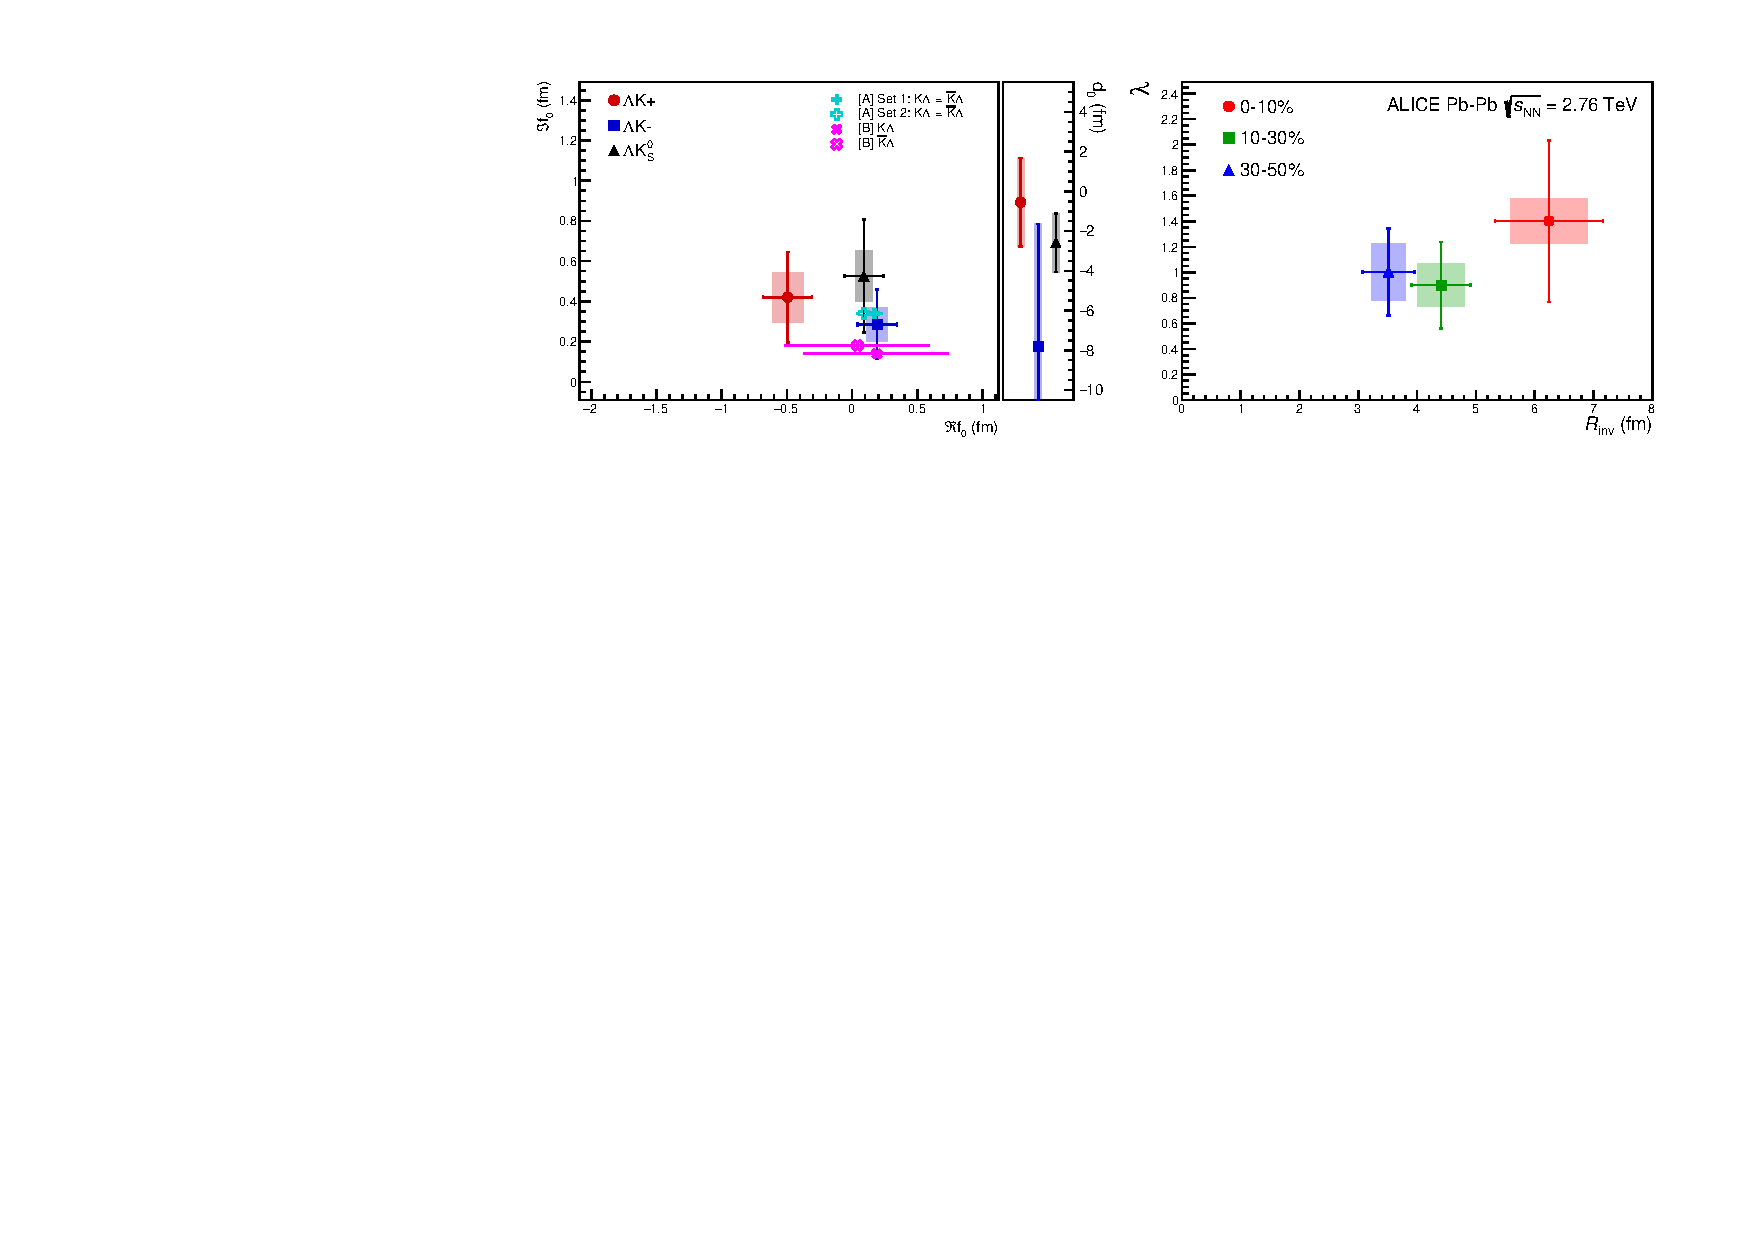
\includegraphics[width=\textwidth]{\ResultsDirBaseLamKch\SaveNameModLamKch/Comparisons/FinalResults_Comp3An.pdf}
   \caption[Extracted Scattering Parameters]
   {
-  Extracted fit parameters for all of the \LamK systems.  
-  [Left]: $\Im f_{0}$ vs. $\Re f_{0}$, together with $d_{0}$ to the right.  
-  [Right]: $\lambda$ vs. Radius for the 0--10\% (blue), 10--30\% (green), and 30--50\% (red) centrality bins.  
+  (Color online) Extracted fit parameters for all of the \LamK systems.  
+  [Left]: $\Im f_{0}$ vs. $\Re f_{0}$, together with $d_{0}$ to the right for the \LamKchP (circles), \LamKchM (squares) and \LamKs (triangles) systems.  
+  [Right]: $\lambda$ vs. Radius for the 0--10\% (circles), 10--30\% (squares), and 30--50\% (triangles) centrality bins.  
   In the fit, all \LamK systems share common radii.
-  The color scheme used in the panel are to be consistent with those in Fig. \ref{fig:mTScalingOfRadii_3Res}.
-  The cyan ([A] = Ref. \cite{Liu:2006xja}) and magenta ([B] = Ref. \cite{Mai:2009ce}) points show theoretical predictions made using chiral perturbation theory.
+  The cross ([A] = Ref.\ \cite{Liu:2006xja}) and X symbols ([B] = Ref.\ \cite{Mai:2009ce}) points show theoretical predictions made using chiral perturbation theory.
   }
   \label{fig:ScattParams_3Res}
 \end{figure}
@@ -980,26 +1016,25 @@
 In the summary plot, the extracted scattering parameters are shown in the form of a $\Im f_{0}$ vs $\Re f_{0}$ plot, which includes the $d_{0}$ values to the right side.  
 Also shown are the $\lambda$ vs. radius parameters for all three studied centrality bins. 
 In addition to the results of this study, theoretical predictions made using chiral perturbation theory \cite{Liu:2006xja,Mai:2009ce} are shown.
-
-For all studied systems, a positive imaginary part, $\Im(f_{0})$, of the scattering lengths are extracted. 
+For all \LamK systems, positive imaginary parts of the scattering lengths, $\Im(f_{0})$, are extracted. 
 This is expected, as $\Im(f_{0})$ describes the inelastic scattering channels.
 More interestingly, the results show that the \LamKchP and \LamKchM systems differ in the sign of the real part, $\Re(f_{0})$, of their scattering lengths, with a negative value for \LamKchP and positive value for \LamKchM.
 The $\Re f_{0}$ extracted for the \LamKs system is positive, and within errors of that of the \LamKchM. 
-Each of the three systems has scattering parameters unique from the others.
 The real part of the scattering length describes the effect of the strong interaction, making the difference in these systems quite intriguing.
-A positive $\Re(f_{0})$ (\LamKchM, \LamKs) signifies that the effect of the strong force is attractive, while a negative $\Re(f_{0})$ (\LamKchP) signifies a repulsion.
-Past studies of kaon-proton scattering found the K$^{-}$-p interaction to be attractive, and that of the K$^{+}$-p to be repulsive.
-With respect to the kaons, this is similar to the current finding of an attractive \Lam-\KchM interaction and a repulsive \Lam-\KchP interaction.
-This difference could be due to an effect arising from different quark-antiquark interactions between the pairs ($\rm s\bar{s}$ in \LamKchP, $\rm u\bar{u}$ in \LamKchM).
+As is the usual convention in femtoscopy, a positive $\Re(f_{0})$ (\LamKchM, \LamKs) signifies that the effect of the interaction is attractive, while a negative $\Re(f_{0})$ (\LamKchP) signifies a repulsive interaction.
+Past studies of kaon-proton scattering found the K$^{-}$--p interaction to be attractive, and that of the K$^{+}$--p to be repulsive \cite{Humphrey:1962zz, Hadjimichef:2002xe, Ikeda:2012au}.
+With respect to the kaons, this is similar to the current finding of an attractive \Lam--\KchM interaction and a repulsive \Lam--\KchP interaction.
+This difference could be due to an effect arising from different quark-antiquark interactions between the pairs ($\rm s\overline{s}$ in \LamKchP, $\rm u\overline{u}$ in \LamKchM).
 A related explanation could be that the effect is due to the different net strangeness for each system.
 
 
 \begin{figure}[h]
   \centering
-  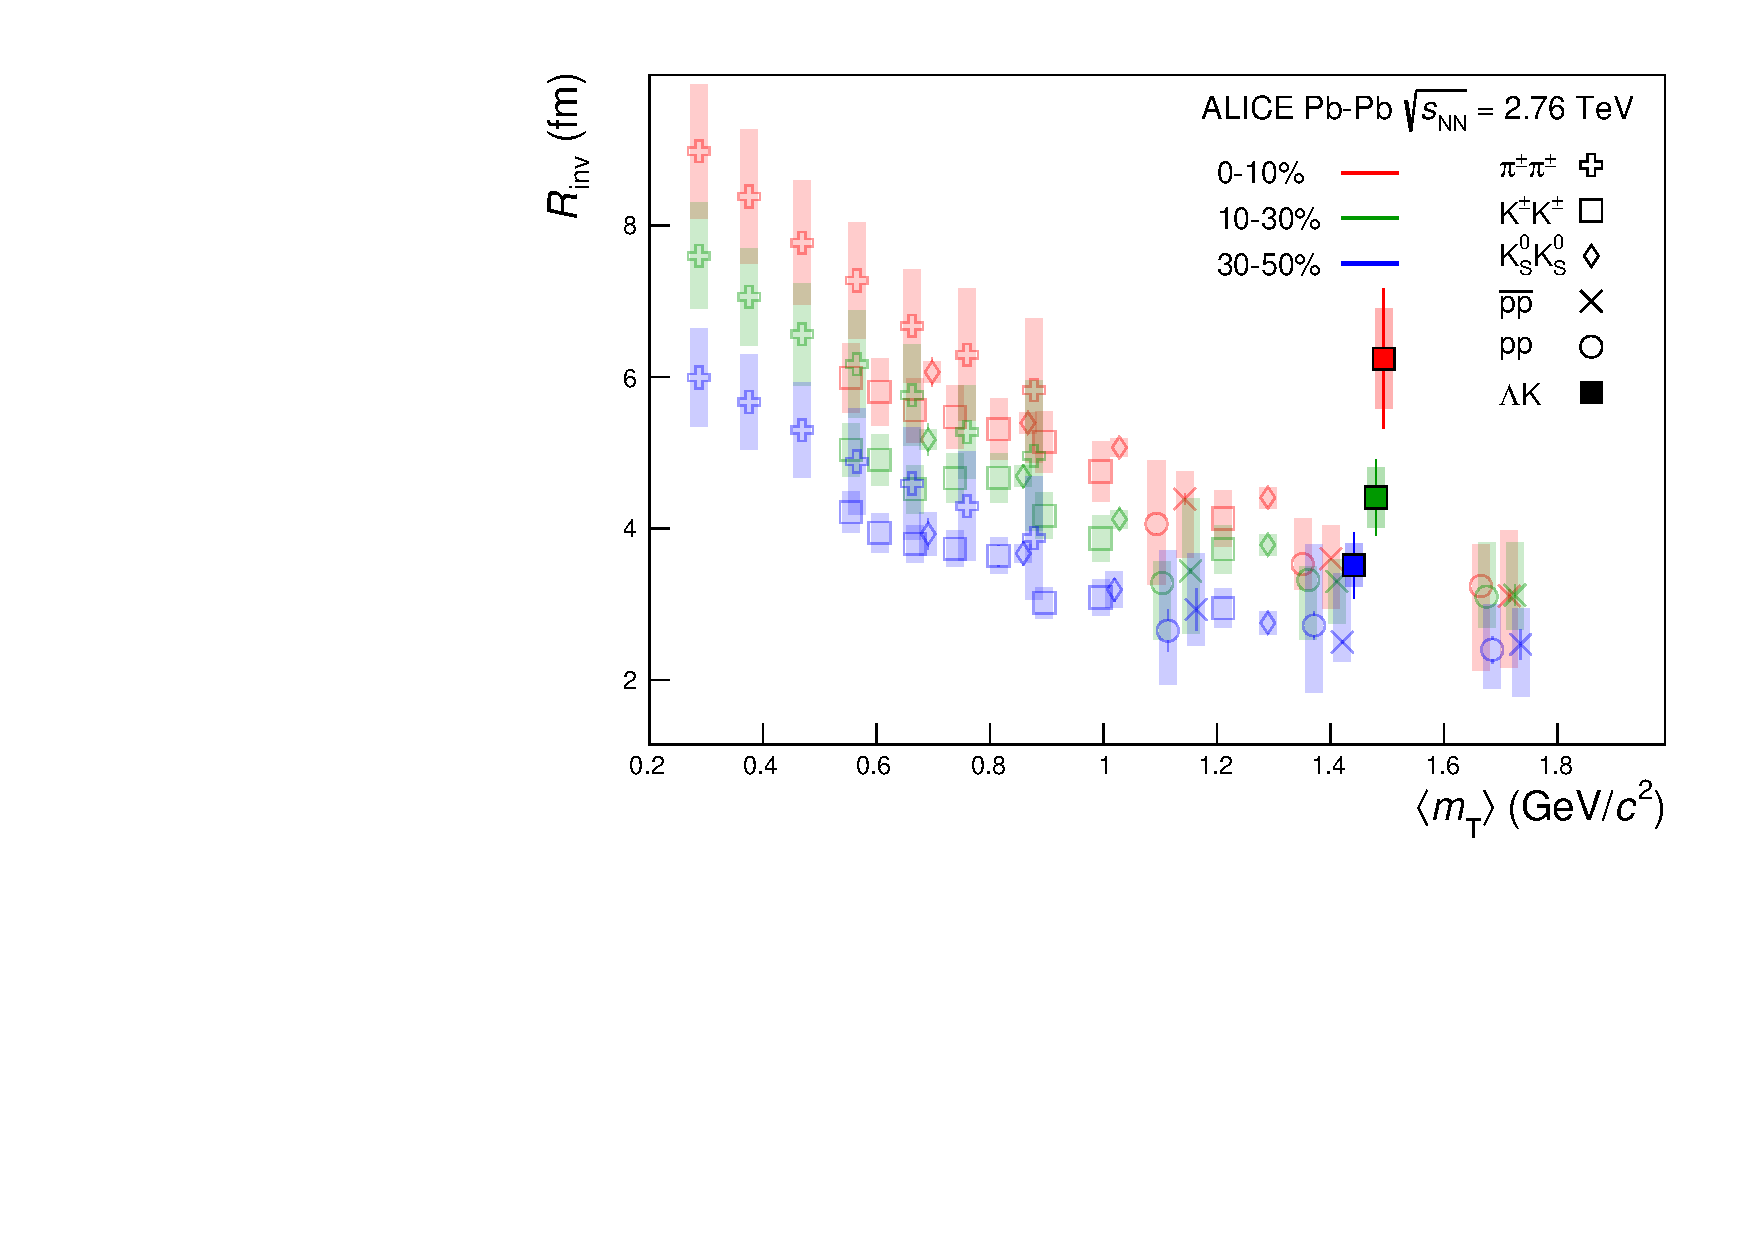
\includegraphics[width=0.75\textwidth]{\ResultsDirBaseLamKch\SaveNameModLamKch/Comparisons/mTscaling_MinvCalc_OutlinedPoints_OthersTransparent_3Res_NoResStamp.pdf}
+  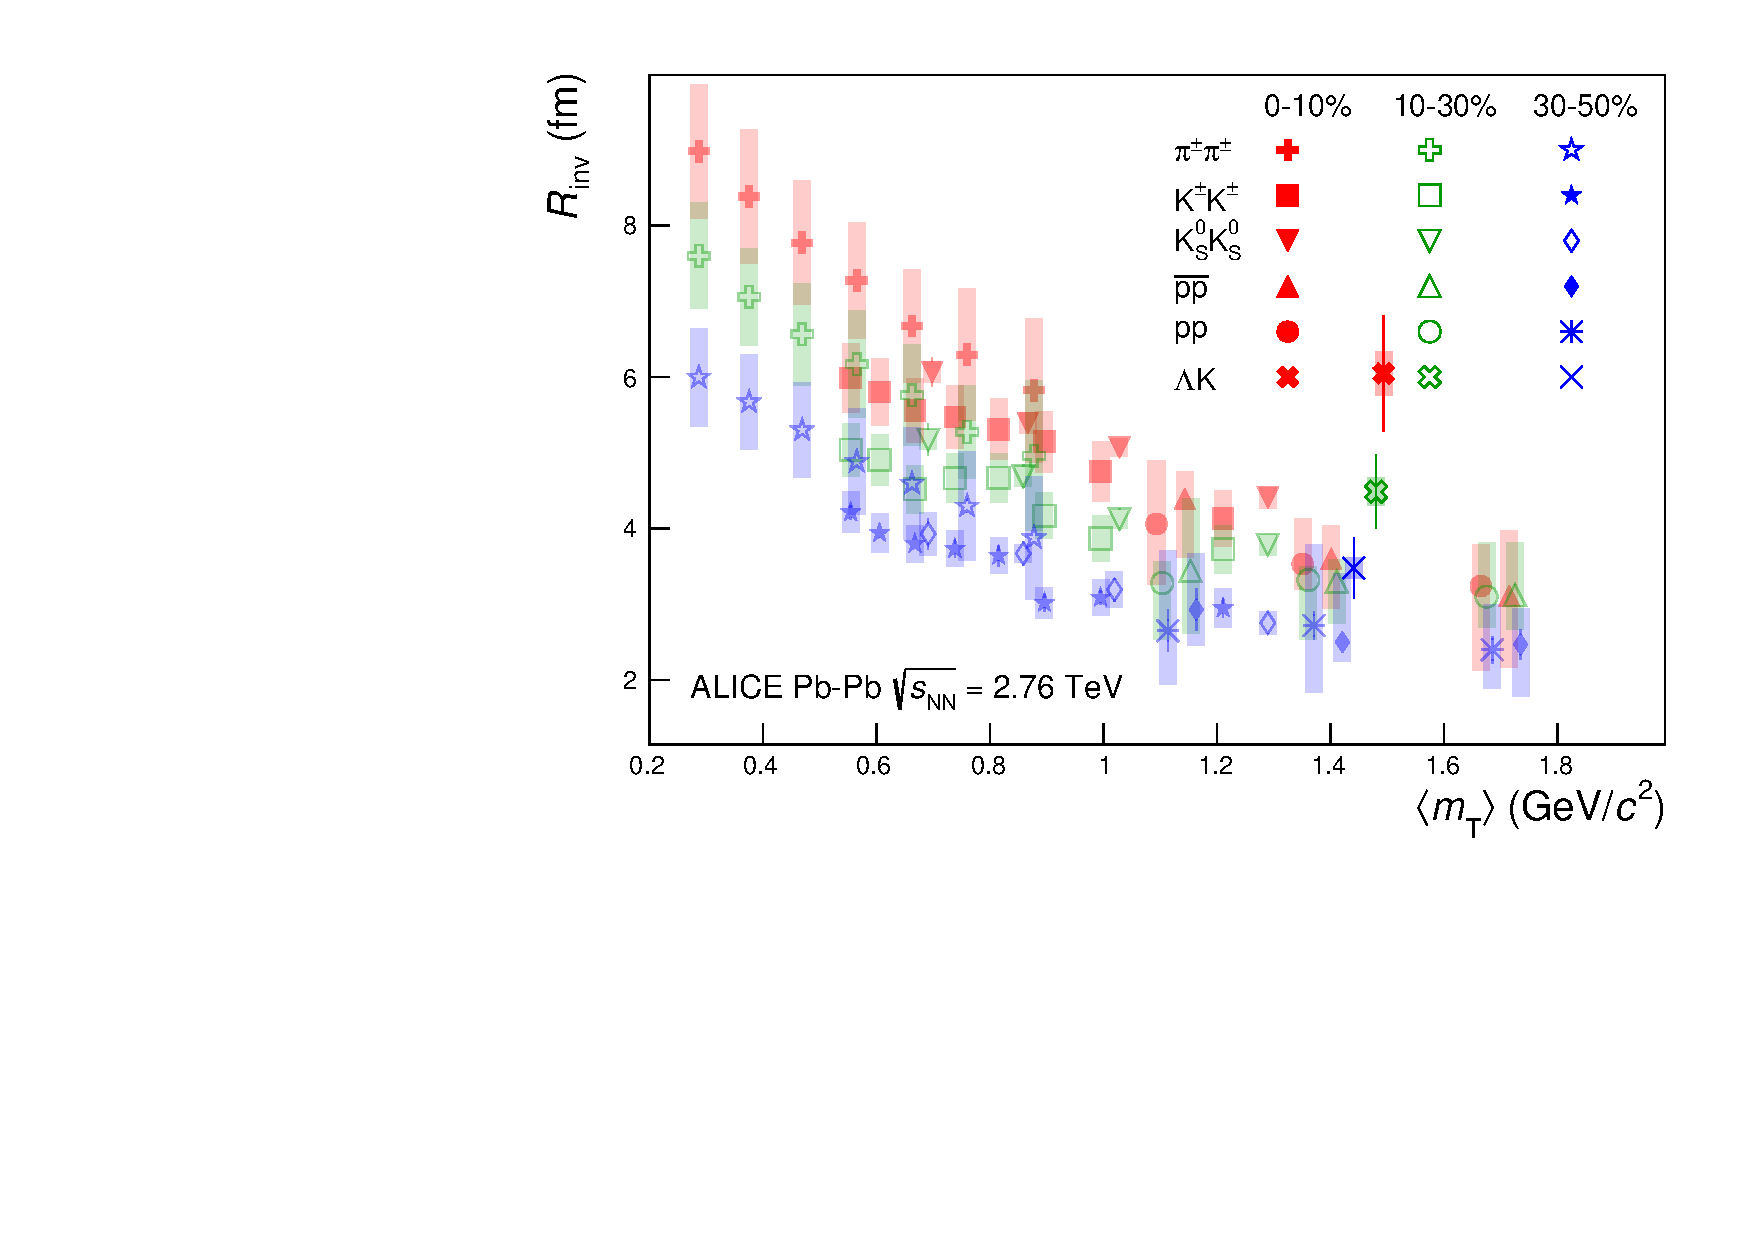
\includegraphics[width=0.75\textwidth]{\ResultsDirBaseLamKch\SaveNameModLamKch/Comparisons/mTscaling_MinvCalcv2_OthersTransparent_3Res_NoResStamp.pdf}
   \caption[\mt Scaling of Radii: 3 Residuals in Fit]
   {
-  Extracted fit $R_{\mathrm{inv}}$ parameters as a function of pair transverse mass (\mt) for various pair systems over several centralities. The ALICE published data \cite{Adam:2015vja} is shown with transparent, open symbols.
+  (Color online) Extracted fit $R_{\mathrm{inv}}$ parameters as a function of pair transverse mass (\mt) for various pair systems over several centralities. 
+  The ALICE published data \cite{Adam:2015vja} is shown with transparent, open symbols.
   }
   \label{fig:mTScalingOfRadii_3Res}
 \end{figure}
@@ -1020,25 +1055,24 @@
 }.
 The radii are observed to increase for more central events, as expected from a simple geometric picture of the collisions.
 They also demonstrate a decreasing size with increasing \mt, as expected in the presence of collective radial flow \cite{Akkelin:1995gh}.
-It was found that \cite{Kisiel:2014upa}, even in the presence of good global \mt-scaling for the three-dimensional radii in the LCMS frame, a particle species dependence will exist for the $R_{\mathrm{inv}}$ measured in the PRF, due to trivial kinematic reasons.
+It was found that \cite{Kisiel:2014upa}, even in the presence of good global \mt-scaling for the three-dimensional radii in the Longitudinally Co-Moving System (LCMS), a particle species dependence will exist for the $R_{\mathrm{inv}}$ measured in the Pair Rest Frame (PRF), due to trivial kinematic reasons.
 These kinematic effects, resulting from the transformation from LCMS to PRF, causes smaller masses to exhibit larger $R_{\mathrm{inv}}$ \cite{Adam:2015vja} (explaining, for instance, how the pion radii are systematically higher than kaon radii at the same approximate \mt).
 
 
-It is clear from the results in Fig. \ref{fig:mTScalingOfRadii_3Res} that the \LamK systems do not conform to the approximate \mt-scaling of the identical particle pair source sizes.
+It is clear from the results in Fig.\ \ref{fig:mTScalingOfRadii_3Res} that the \LamK systems do not conform to the approximate \mt-scaling of the identical particle pair source sizes.
 At first thought, this may appear to be a troubling result; the approximate scaling is an observed consequence of the collective behavior of the soft (low-\pt) sector of the produced system.
-The \Lam and K particles certainly participate in the collective expansion of the QGP medium, but, importantly, they are non-identical particles, and all other systems in Fig. \ref{fig:mTScalingOfRadii_3Res} contain identical particles.
+The \Lam and K particles certainly participate in the collective expansion of the QGP medium, but, importantly, they are non-identical particles, and all other systems in Fig.\ \ref{fig:mTScalingOfRadii_3Res} contain identical particles.
 In the case of identical particle femtoscopy, the pair source is comprised of two identical single particle sources, and the pair source size extracted is simply a factor $\sqrt{2}$ larger than those single particle sources.
 Thus, the identical particle pair source radii naturally follow the single particle source \mt-scaling in a simple manner.
 
 When dealing with non-identical particles, the pair emission source, which is measured by femtoscopy, is the superposition of two single-particle sources.
-In general, each single-particle source will have its own size, shape, and space-time position within the produced medium, which is unique from its paired partner.
 The hydrodynamic nature of the medium produces the approximate \mt-scaling with respect to these single-particle sources, not the pair sources.
-More specifically, the hydrodynamic response of the system confines higher-\mt particles to smaller homogeneity regions, also also pushes their average emission points further in the ``out" direction \cite{Retiere:2003kf}.
+More specifically, the hydrodynamic response of the system confines higher-\mt particles to smaller homogeneity regions, also pushes their average emission points further in the ``out" direction \cite{Retiere:2003kf}.
 Therefore, it is expected that the \Lam source is both smaller in size and further out in the fireball than that of the kaons.
 The combination of two unique sources separated in space-time, when probing correlations between non-identical particle pairs, can lead to extracted radii falling outside of the (identical particle femtoscopy) \mt-scaling trend.
 
 It is well established that non-identical particle femtoscopic studies are able to probe deeper than the second moments of the pair distribution functions accessed via identical particle studies.
-In addition to this, non-identical particle studies are able to measure the relative emission shifts, the first moments of the emission function.
+In addition to this, non-identical particle studies are able to measure the relative emission shifts, the first moments of the emission function \cite{Kisiel:2009eh}.
 For the study of \LamK pairs at mid-rapidity in Pb-Pb collisions, a separation of the single-particle sources in the out direction is expected.
 One elegant method for extracting information about the emission asymmetries is via a spherical decomposition of the correlation function.
 With this method, one can draw a wealth of information from just a few components of the decomposition.
@@ -1048,17 +1082,20 @@
 
 Figure \ref{fig:LamKchP_ReC00C11_0010} shows the $C_{00}$ and $\Re C_{11}$ components from the spherical decomposition of the \LamKchP data in the 0--10\% centrality bin.
 The $\Re C_{11}$ component shows a clear deviation from zero, and the negative value signifies that the \Lam particles are, on average, emitted further out and/or earlier than the K mesons.
-This effect is supported by the results obtained from the THERMINATOR 2 model, shown in Fig. \ref{fig:LamKchP_StdThermSources}.
+This effect is supported by the results obtained from the THERMINATOR 2 model, shown in Fig.\ \ref{fig:LamKchP_StdThermSources}.
 The effect of a non-zero shift in the source will naturally lead to larger measured radii.
-This is intuitive, and also reaffirmed in the simulation with THERMINATOR 2 shown in App. \ref{App:THERM}.
+This is intuitive, and also reaffirmed in the simulation with THERMINATOR 2 shown in App.\ \ref{App:THERM}.
 Larger effective radii are also found to result from inserting a Gaussian source with a non-zero shift into the Koonin-Pratt equation and numerically integrating.
 
 \begin{figure}[h!]
   \centering
   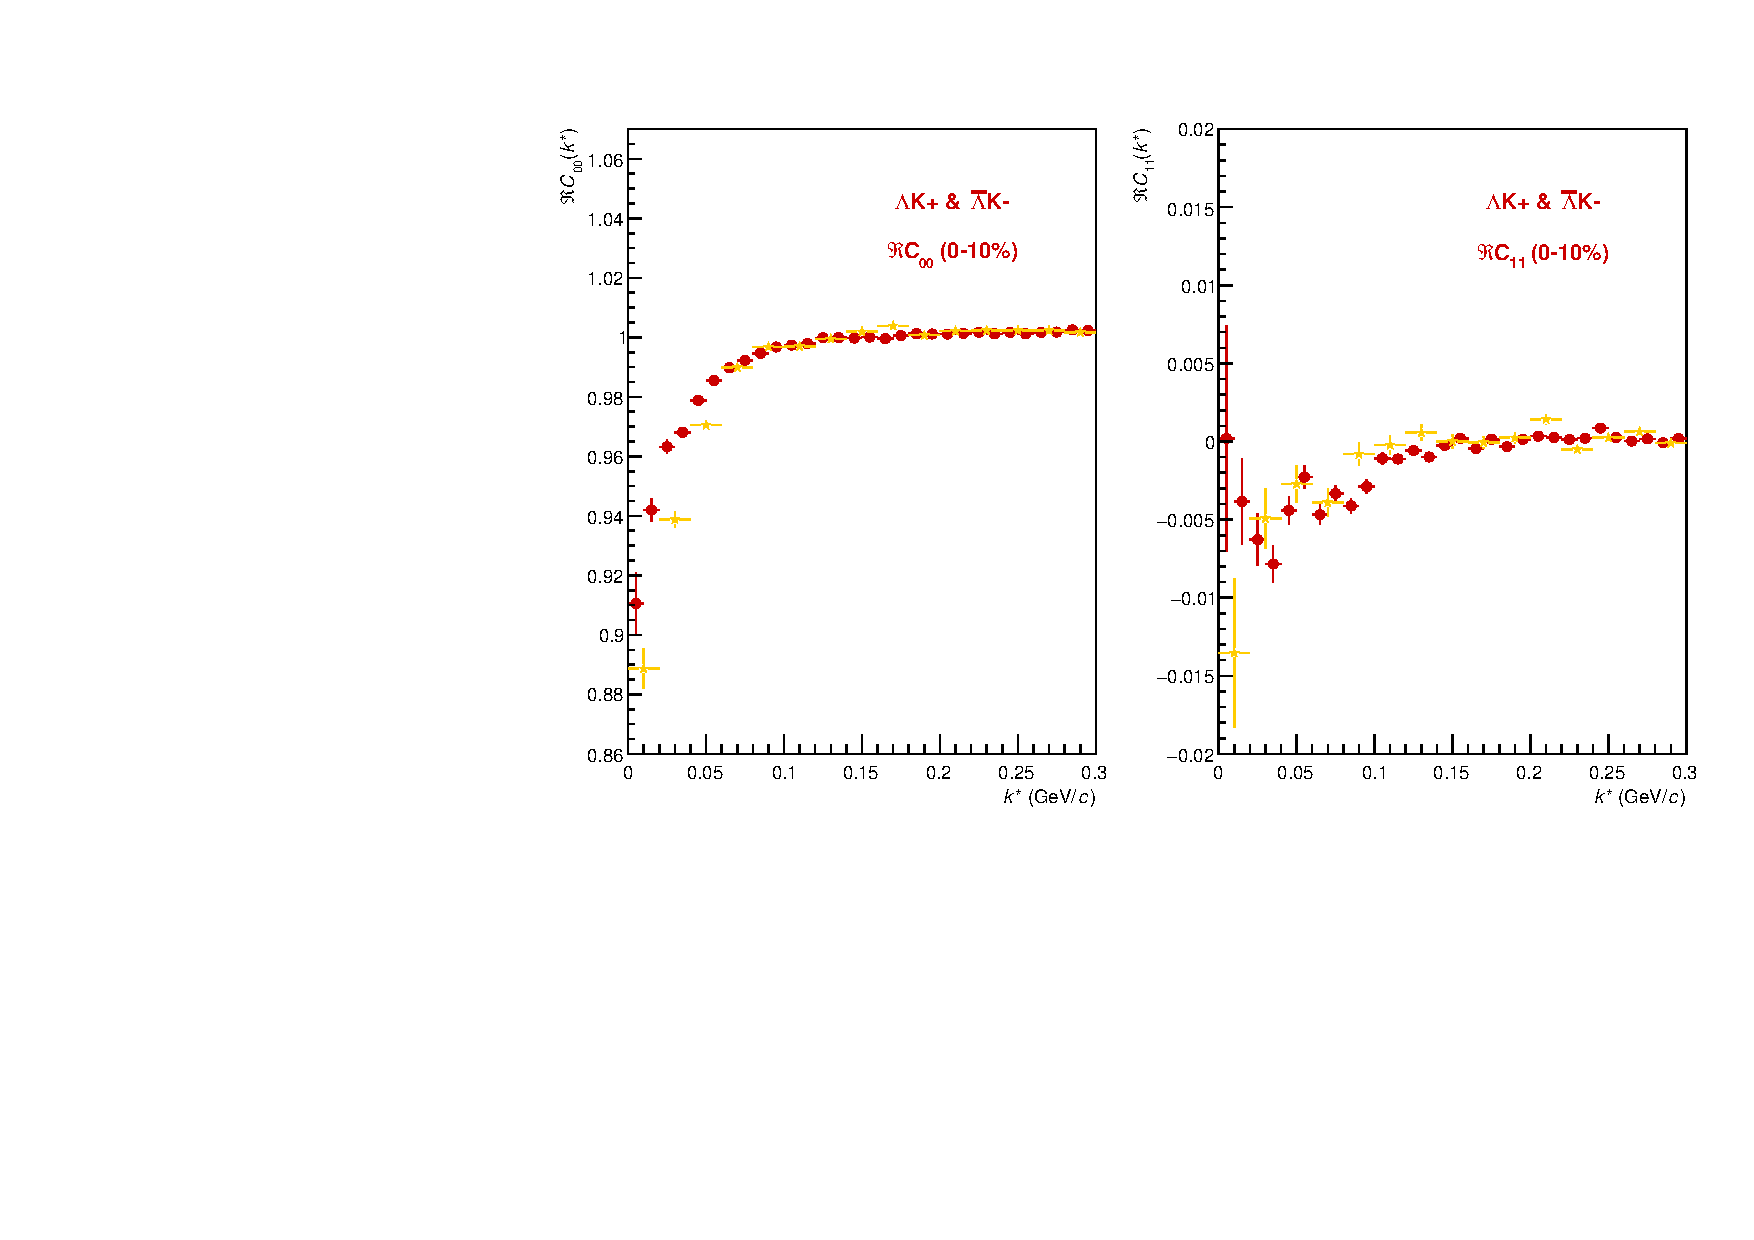
\includegraphics[width=0.8\textwidth]{\ResultsDirBase Results_cLamcKch_20181205/SphericalHarmonics/LamKchP/CanCfYlmReC00C11_LamKchPALamKchM_0010.pdf}
-  \caption[\LamKchP $C_{00}$ and $\Re C_{11}$ Spherical Harmonic Components (0--10\%)]{$C_{00}$ (left) and $\Re C_{11}$ (right) components of a spherical harmonic decomposition of the \LamKchP correlation function for the 0--10\% centrality bin.  
+  \caption[\LamKchP $C_{00}$ and $\Re C_{11}$ Spherical Harmonic Components (0--10\%)]
+  {
+  (Color online) $C_{00}$ (left) and $\Re C_{11}$ (right) components of a spherical harmonic decomposition of the \LamKchP correlation function for the 0--10\% centrality bin.  
 The $C_{00}$ component is similar to the 1D correlation functions typically studied, and probes the overall size of the source.
-The $\Re C_{11}$ component probes the asymmetry in the system; a non-zero value reveals the asymmetry}
+The $\Re C_{11}$ component probes the asymmetry in the system; a non-zero value reveals the asymmetry
+  }
   \label{fig:LamKchP_ReC00C11_0010}
 \end{figure}
 
@@ -1074,10 +1111,8 @@
 Results from a femtoscopic analysis of \LamK correlations in Pb-Pb collisions at $\sqrt{s_{\mathrm{NN}}}$ = 2.76 TeV with ALICE at the LHC have been presented.
 The femtoscopic radii, $\lambda$ parameters, and scattering parameters were extracted from one-dimensional correlation functions in terms of the invariant momentum difference.
 The scattering parameters of \LamK pairs in all three charge combinations (\LamKchP, \LamKchM, and \LamKs) have been measured for the first time.
-A striking difference in the \LamKchP and \LamKchM correlation functions is observed, which is reflected in the unique set of scattering parameters extracted for each.
-The \LamKs systems is somewhat intermediate to these two cases.
-The \LamKchP systems exhibits a negative $\Re(f_{0})$, while those extracted from the \LamKchM and \LamKs systems are positive.
-This implies that the strong interaction is repulsive for the \LamKchP system and attractive for \LamKchM and \LamKs.
+Striking differences are observed in the \LamKchP, \LamKchM, and \LamKs correlation functions, which are reflected in the unique set of scattering parameters extracted for each.
+The extracted scattering parameters indicate that the strong force is repulsive in the \LamKchP interaction and attractive in the \LamKchM and \LamKs interactions.
 The physics underlying this phenomenon is currently not well understood, but this could be due to different quark-antiquark interactions between the pairs, or from different net strangeness for each system. 
 The non-femtoscopic background is found to result almost entirely from collective effects, and is described quantitatively with unprecedented precision with the THERMINATOR 2 event generator.
 Finally, the \LamK systems exhibit source radii larger than expected from extrapolation from identical particle femtoscopic studies.
@@ -1128,11 +1163,11 @@
   \hlineB{3.0}
   Primary & 0.527 & Primary & 0.526 & Primary & 0.526 & Primary & 0.527 & Primary & 0.543 & Primary & 0.544 \\
   
-  $\Sigma^{0}$K$^{+}$ & 0.111 & $\bar{\Sigma}^{0}$K$^{-}$ & 0.110 & $\Sigma^{0}$K$^{-}$ & 0.110 & $\bar{\Sigma}^{0}$K$^{+}$ & 0.111 & $\Sigma^{0}$K$^{0}_{\mathrm{S}}$ & 0.120 & $\bar{\Sigma}^{0}$K$^{0}_{\mathrm{S}}$ & 0.120 \\
-  
-  $\Xi^{0}$K$^{+}$ & 0.039 & $\bar{\Xi}^{0}$K$^{-}$ & 0.035 & $\Xi^{0}$K$^{-}$ & 0.038 & $\bar{\Xi}^{0}$K$^{+}$ & 0.036 & $\Xi^{0}$K$^{0}_{\mathrm{S}}$ & 0.042 & $\bar{\Xi}^{0}$K$^{0}_{\mathrm{S}}$ & 0.039 \\
-  
-  $\Xi^{-}$K$^{+}$ & 0.050 & $\bar{\Xi}^{+}$K$^{-}$ & 0.046 & $\Xi^{-}$K$^{-}$ & 0.050 & $\bar{\Xi}^{+}$K$^{+}$ & 0.046 & $\Xi^{-}$K$^{0}_{\mathrm{S}}$ & 0.054 & $\bar{\Xi}^{+}$K$^{0}_{\mathrm{S}}$ & 0.050 \\
+  $\Sigma^{0}$K$^{+}$ & 0.111 & $\overline{\Sigma}^{0}$K$^{-}$ & 0.110 & $\Sigma^{0}$K$^{-}$ & 0.110 & $\overline{\Sigma}^{0}$K$^{+}$ & 0.111 & $\Sigma^{0}$K$^{0}_{\mathrm{S}}$ & 0.120 & $\overline{\Sigma}^{0}$K$^{0}_{\mathrm{S}}$ & 0.120 \\
+  
+  $\Xi^{0}$K$^{+}$ & 0.039 & $\overline{\Xi}^{0}$K$^{-}$ & 0.035 & $\Xi^{0}$K$^{-}$ & 0.038 & $\overline{\Xi}^{0}$K$^{+}$ & 0.036 & $\Xi^{0}$K$^{0}_{\mathrm{S}}$ & 0.042 & $\overline{\Xi}^{0}$K$^{0}_{\mathrm{S}}$ & 0.039 \\
+  
+  $\Xi^{-}$K$^{+}$ & 0.050 & $\overline{\Xi}^{+}$K$^{-}$ & 0.046 & $\Xi^{-}$K$^{-}$ & 0.050 & $\overline{\Xi}^{+}$K$^{+}$ & 0.046 & $\Xi^{-}$K$^{0}_{\mathrm{S}}$ & 0.054 & $\overline{\Xi}^{+}$K$^{0}_{\mathrm{S}}$ & 0.050 \\
   
   Other & 0.226 & Other & 0.235 & Other & 0.228 & Other & 0.233 & Other & 0.194 & Other & 0.199 \\
   
@@ -1143,25 +1178,25 @@
   \hlineB{3.0}
   Primary & 0.180 & Primary & 0.180 & Primary & 0.179 & Primary & 0.181 & Primary & 0.192 & Primary & 0.193 \\
   
-  $\Sigma^{0}$K$^{+}$ & 0.116 & $\bar{\Sigma}^{0}$K$^{-}$ & 0.114 & $\Sigma^{0}$K$^{-}$ & 0.115 & $\bar{\Sigma}^{0}$K$^{+}$ & 0.116 & $\Sigma^{0}$K$^{0}_{\mathrm{S}}$ & 0.125 & $\bar{\Sigma}^{0}$K$^{0}_{\mathrm{S}}$ & 0.124 \\
-  
-  $\Xi^{0}$K$^{+}$ & 0.040 & $\bar{\Xi}^{0}$K$^{-}$ & 0.037 & $\Xi^{0}$K$^{-}$ & 0.040 & $\bar{\Xi}^{0}$K$^{+}$ & 0.037 & $\Xi^{0}$K$^{0}_{\mathrm{S}}$ & 0.043 & $\bar{\Xi}^{0}$K$^{0}_{\mathrm{S}}$ & 0.040 \\
-  
-  $\Xi^{-}$K$^{+}$ & 0.052 & $\bar{\Xi}^{+}$K$^{-}$ & 0.047 & $\Xi^{-}$K$^{-}$ & 0.052 & $\bar{\Xi}^{+}$K$^{+}$ & 0.048 & $\Xi^{-}$K$^{0}_{\mathrm{S}}$ & 0.056 & $\bar{\Xi}^{+}$K$^{0}_{\mathrm{S}}$ & 0.052 \\
-  
-  $\Sigma^{*+}$K$^{+}$ & 0.054 & $\bar{\Sigma}^{*-}$K$^{-}$ & 0.051 & $\Sigma^{*+}$K$^{-}$ & 0.053 & $\bar{\Sigma}^{*-}$K$^{+}$ & 0.051 & $\Sigma^{*+}$K$^{0}_{\mathrm{S}}$ & 0.058 & $\bar{\Sigma}^{*-}$K$^{0}_{\mathrm{S}}$ & 0.055 \\
-  
-  $\Sigma^{*-}$K$^{+}$ & 0.048 & $\bar{\Sigma}^{*+}$K$^{-}$ & 0.050 & $\Sigma^{*-}$K$^{-}$ & 0.048 & $\bar{\Sigma}^{*+}$K$^{+}$ & 0.050 & $\Sigma^{*-}$K$^{0}_{\mathrm{S}}$ & 0.052 & $\bar{\Sigma}^{*+}$K$^{0}_{\mathrm{S}}$ & 0.054 \\
-  
-  $\Sigma^{*0}$K$^{+}$ & 0.048 & $\bar{\Sigma}^{*0}$K$^{-}$ & 0.045 & $\Sigma^{*0}$K$^{-}$ & 0.048 & $\bar{\Sigma}^{*0}$K$^{+}$ & 0.045 & $\Sigma^{*0}$K$^{0}_{\mathrm{S}}$ & 0.052 & $\bar{\Sigma}^{*0}$K$^{0}_{\mathrm{S}}$ & 0.048 \\
-  
-  $\Lambda$K$^{*0}$ & 0.046 & $\bar{\Lambda}\bar{\mathrm{K}}^{*0}$ & 0.047 & $\Lambda\bar{\mathrm{K}}^{*0}$ & 0.046 & $\bar{\Lambda}$K$^{*0}$ & 0.047 & $\Lambda$K$^{*0}$ & 0.022 & $\bar{\Lambda}$K$^{*0}$ & 0.022 \\
-  
-  $\Sigma^{0}$K$^{*0}$ & 0.041 & $\bar{\Sigma}^{0}\bar{\mathrm{K}}^{*0}$ & 0.041 & $\Sigma^{0}\bar{\mathrm{K}}^{*0}$ & 0.041 & $\bar{\Sigma}^{0}$K$^{*0}$ & 0.041 & $\Sigma^{0}$K$^{*0}$ & 0.019 & $\bar{\Sigma}^{0}$K$^{*0}$ & 0.019 \\
-  
-  $\Xi^{0}$K$^{*0}$ & 0.014 & $\bar{\Xi}^{0}\bar{\mathrm{K}}^{*0}$ & 0.013 & $\Xi^{0}\bar{\mathrm{K}}^{*0}$ & 0.014 & $\bar{\Xi}^{0}$K$^{*0}$ & 0.013 & $\Xi^{0}$K$^{*0}$ & 0.007 & $\bar{\Xi}^{0}$K$^{*0}$ & 0.006 \\
-  
-  $\Xi^{-}$K$^{*0}$ & 0.018 & $\bar{\Xi}^{+}\bar{\mathrm{K}}^{*0}$ & 0.017 & $\Xi^{-}\bar{\mathrm{K}}^{*0}$ & 0.018 & $\bar{\Xi}^{+}$K$^{*0}$ & 0.017 & $\Xi^{-}$K$^{*0}$ & 0.009 & $\bar{\Xi}^{+}$K$^{*0}$ & 0.008 \\
+  $\Sigma^{0}$K$^{+}$ & 0.116 & $\overline{\Sigma}^{0}$K$^{-}$ & 0.114 & $\Sigma^{0}$K$^{-}$ & 0.115 & $\overline{\Sigma}^{0}$K$^{+}$ & 0.116 & $\Sigma^{0}$K$^{0}_{\mathrm{S}}$ & 0.125 & $\overline{\Sigma}^{0}$K$^{0}_{\mathrm{S}}$ & 0.124 \\
+  
+  $\Xi^{0}$K$^{+}$ & 0.040 & $\overline{\Xi}^{0}$K$^{-}$ & 0.037 & $\Xi^{0}$K$^{-}$ & 0.040 & $\overline{\Xi}^{0}$K$^{+}$ & 0.037 & $\Xi^{0}$K$^{0}_{\mathrm{S}}$ & 0.043 & $\overline{\Xi}^{0}$K$^{0}_{\mathrm{S}}$ & 0.040 \\
+  
+  $\Xi^{-}$K$^{+}$ & 0.052 & $\overline{\Xi}^{+}$K$^{-}$ & 0.047 & $\Xi^{-}$K$^{-}$ & 0.052 & $\overline{\Xi}^{+}$K$^{+}$ & 0.048 & $\Xi^{-}$K$^{0}_{\mathrm{S}}$ & 0.056 & $\overline{\Xi}^{+}$K$^{0}_{\mathrm{S}}$ & 0.052 \\
+  
+  $\Sigma^{*+}$K$^{+}$ & 0.054 & $\overline{\Sigma}^{*-}$K$^{-}$ & 0.051 & $\Sigma^{*+}$K$^{-}$ & 0.053 & $\overline{\Sigma}^{*-}$K$^{+}$ & 0.051 & $\Sigma^{*+}$K$^{0}_{\mathrm{S}}$ & 0.058 & $\overline{\Sigma}^{*-}$K$^{0}_{\mathrm{S}}$ & 0.055 \\
+  
+  $\Sigma^{*-}$K$^{+}$ & 0.048 & $\overline{\Sigma}^{*+}$K$^{-}$ & 0.050 & $\Sigma^{*-}$K$^{-}$ & 0.048 & $\overline{\Sigma}^{*+}$K$^{+}$ & 0.050 & $\Sigma^{*-}$K$^{0}_{\mathrm{S}}$ & 0.052 & $\overline{\Sigma}^{*+}$K$^{0}_{\mathrm{S}}$ & 0.054 \\
+  
+  $\Sigma^{*0}$K$^{+}$ & 0.048 & $\overline{\Sigma}^{*0}$K$^{-}$ & 0.045 & $\Sigma^{*0}$K$^{-}$ & 0.048 & $\overline{\Sigma}^{*0}$K$^{+}$ & 0.045 & $\Sigma^{*0}$K$^{0}_{\mathrm{S}}$ & 0.052 & $\overline{\Sigma}^{*0}$K$^{0}_{\mathrm{S}}$ & 0.048 \\
+  
+  $\Lambda$K$^{*0}$ & 0.046 & $\overline{\Lambda}\overline{\mathrm{K}}^{*0}$ & 0.047 & $\Lambda\overline{\mathrm{K}}^{*0}$ & 0.046 & $\overline{\Lambda}$K$^{*0}$ & 0.047 & $\Lambda$K$^{*0}$ & 0.022 & $\overline{\Lambda}$K$^{*0}$ & 0.022 \\
+  
+  $\Sigma^{0}$K$^{*0}$ & 0.041 & $\overline{\Sigma}^{0}\overline{\mathrm{K}}^{*0}$ & 0.041 & $\Sigma^{0}\overline{\mathrm{K}}^{*0}$ & 0.041 & $\overline{\Sigma}^{0}$K$^{*0}$ & 0.041 & $\Sigma^{0}$K$^{*0}$ & 0.019 & $\overline{\Sigma}^{0}$K$^{*0}$ & 0.019 \\
+  
+  $\Xi^{0}$K$^{*0}$ & 0.014 & $\overline{\Xi}^{0}\overline{\mathrm{K}}^{*0}$ & 0.013 & $\Xi^{0}\overline{\mathrm{K}}^{*0}$ & 0.014 & $\overline{\Xi}^{0}$K$^{*0}$ & 0.013 & $\Xi^{0}$K$^{*0}$ & 0.007 & $\overline{\Xi}^{0}$K$^{*0}$ & 0.006 \\
+  
+  $\Xi^{-}$K$^{*0}$ & 0.018 & $\overline{\Xi}^{+}\overline{\mathrm{K}}^{*0}$ & 0.017 & $\Xi^{-}\overline{\mathrm{K}}^{*0}$ & 0.018 & $\overline{\Xi}^{+}$K$^{*0}$ & 0.017 & $\Xi^{-}$K$^{*0}$ & 0.009 & $\overline{\Xi}^{+}$K$^{*0}$ & 0.008 \\
   
   Other & 0.295 & Other & 0.310 & Other & 0.299 & Other & 0.307 & Other & 0.318 & Other & 0.330 \\
   
@@ -1188,33 +1223,43 @@
 More specifically, the intent is to handle background contributions from elliptic flow, and other sources having reflection symmetry in the transverse plane.  
 With the Stavinskiy method, mixed-event pairs are not used for the reference distribution; instead, same-event pseudo-pairs, formed by rotating one particle in a real pair by 180$^\circ$ in the transverse plane, are used.  
 This rotation rids the pairs of any femtoscopic correlation, while maintaining correlations due to elliptic flow (and other suitably symmetric contributors).
-
+Care needs to be taken in treating the pseudo-pairs exactly like the real pairs; e.g. the pseudo-pairs should be exposed to the same pair cuts used in the analysis on the real pairs.
 The results of correctly implementing such a procedure are shown in Figure \ref{fig:StavCfs_Correct_LamKchP}.  
-The figure shows the Stavinskiy method does a very good job of ridding the \LamKpm correlations of their non-femtoscopic backgrounds.  
-However, the procedure does not work as well on the \LamKs system.
-
-
+The figure shows the Stavinskiy method does a very good job of ridding the \LamKchP correlations of their non-femtoscopic backgrounds.  
+
+%%%%%%%%%%%%%%%%%%%%%%%%%%%%%%%%%%%%%%%%%%%%%%%%%%%%%%%%%%%%%%%%%%%%%%%%%%%%%%%%%%%%%%%%%%%%%%%%%%%%%%%%%%%%%
+\begin{comment}
 \begin{figure}[h!]
   \centering
-  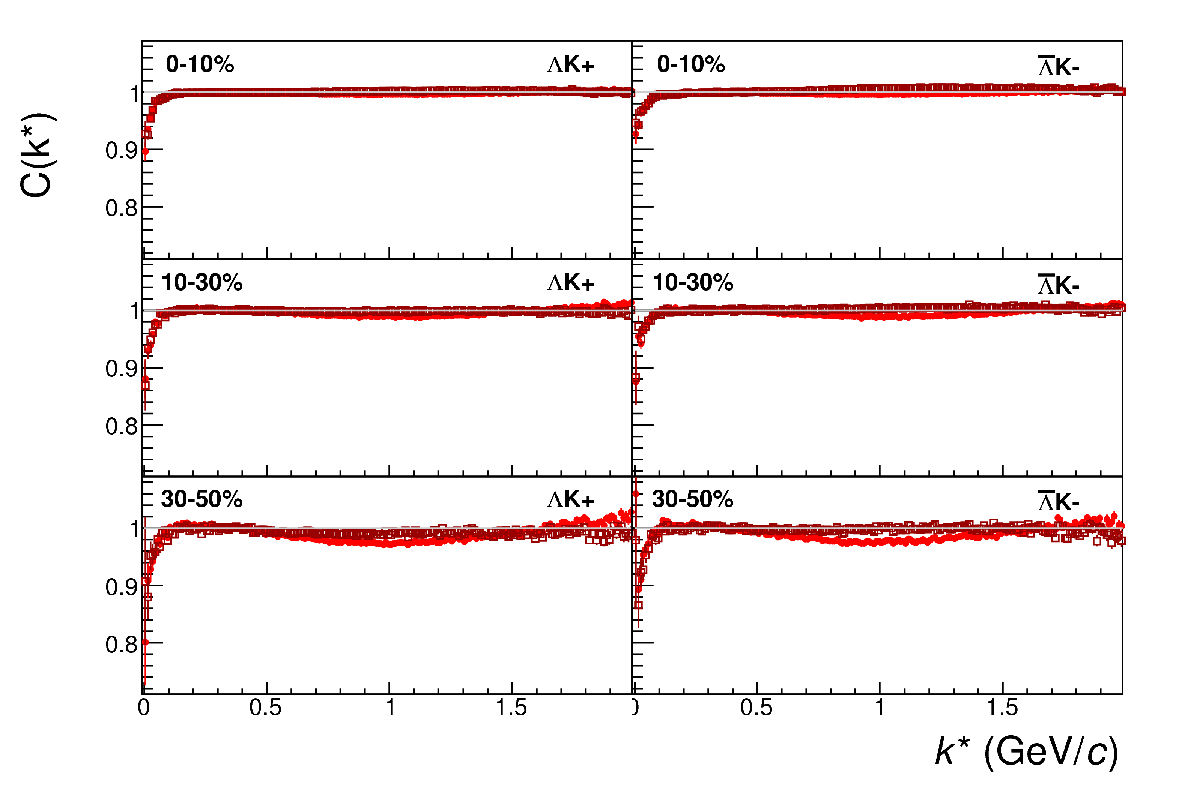
\includegraphics[width=\textwidth]{/home/jesse/Analysis/FemtoAnalysis/AnalysisNotes/4_CorrelationFunctions/Figures/WithAdditionalPairCut_20180505/canKStarCfsLamKchPwConj_20180505vs20180505StavCf.pdf}
-  \caption[\LamKchP Stavinskiy Correlation Functions]{\LamKchPALamKchM correlation functions built using the Stavinskiy method for 0--10\%, 10--30\%, and 30--50\% centralities.  Closed symbols represent correlations built using the normal mixed-event reference distribution, while open symbols represent correlations formed using the Stavinskiy same-event pseudo-pairs as a reference.}
+  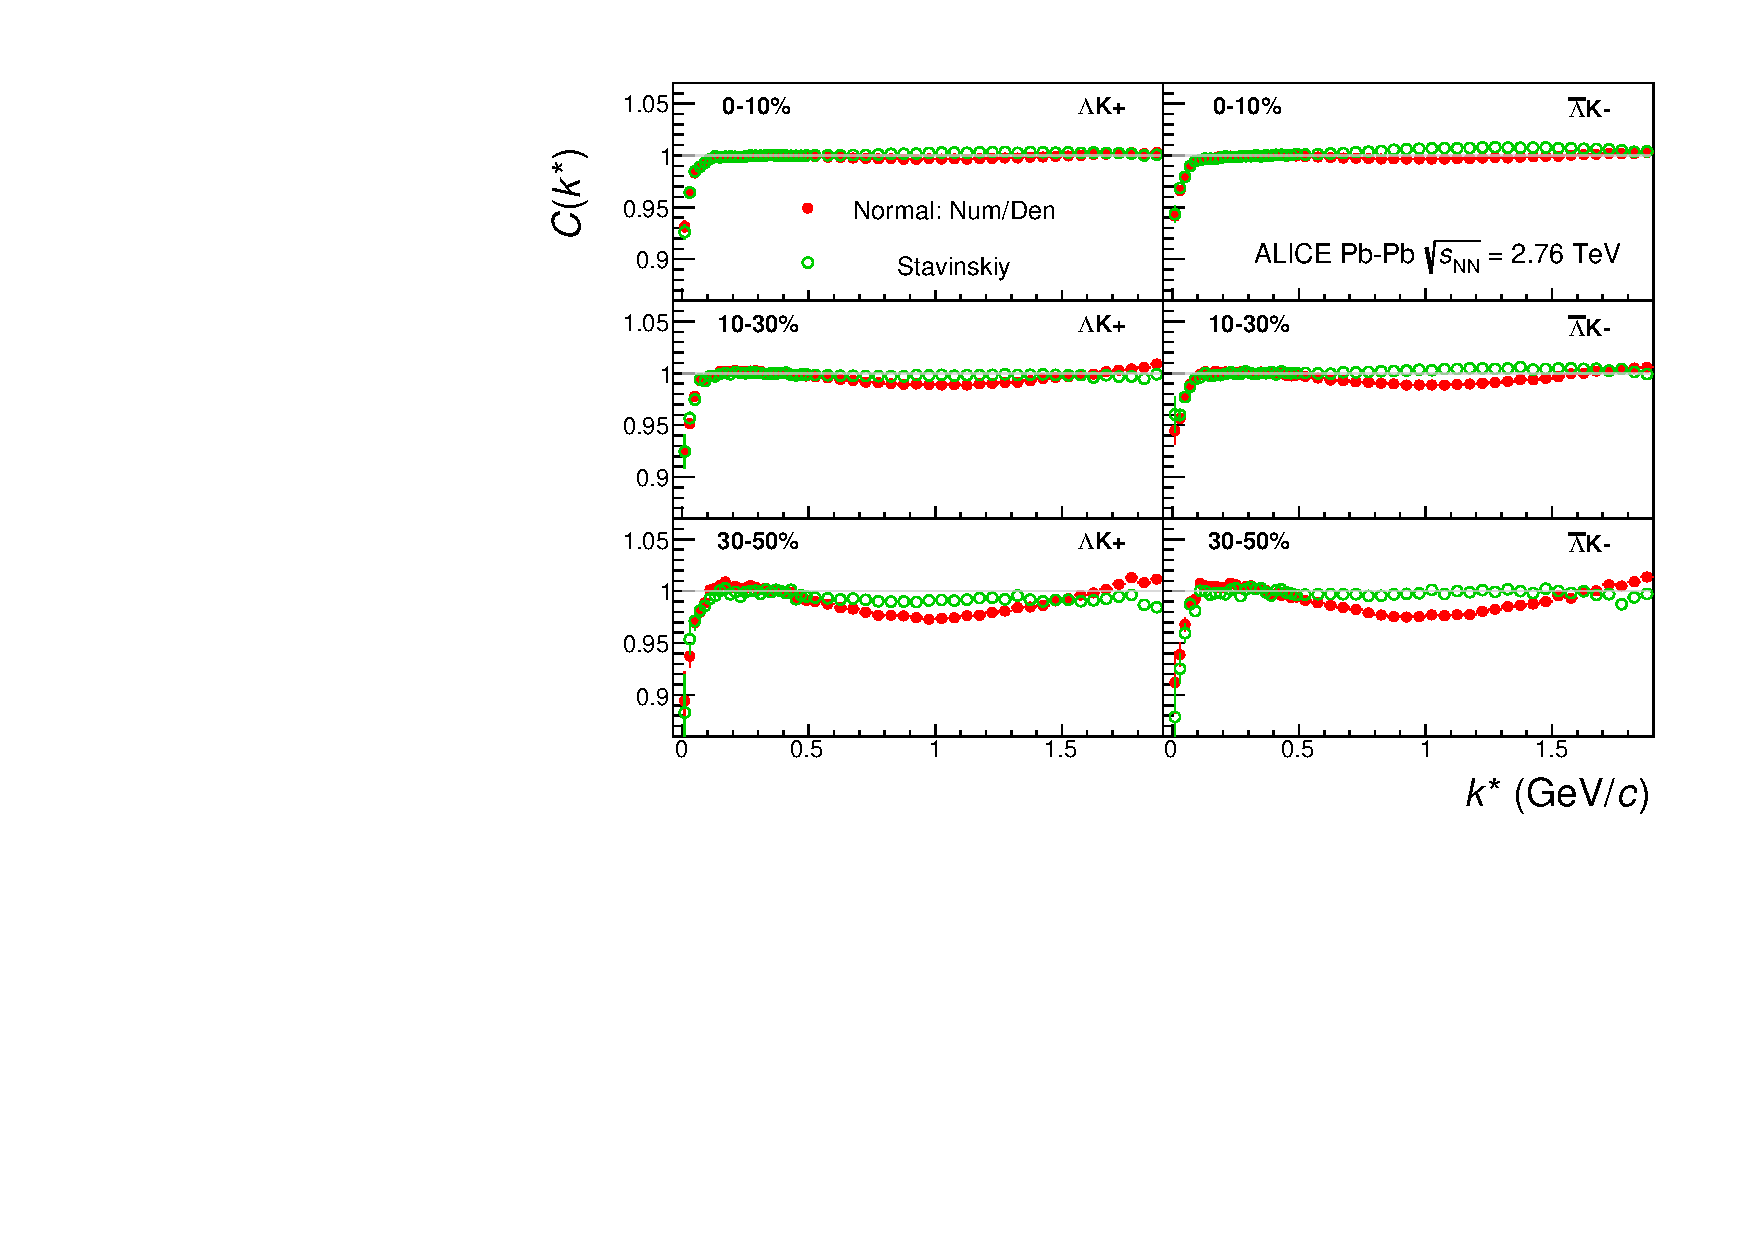
\includegraphics[width=\textwidth]{/home/jesse/Analysis/FemtoAnalysis/AnalysisNotes/4_CorrelationFunctions/Figures/OnlyTwo/canKStarCfsLamKchPwConj_20180505vs20180505StavCf_CustomRebin.pdf}
+  \caption[\LamKchP Stavinskiy Correlation Functions]
+  {
+  \LamKchPALamKchM correlation functions built using the Stavinskiy method for 0--10\%, 10--30\%, and 30--50\% centralities.  
+  Closed (red) symbols represent correlations built using the normal mixed-event reference distribution, while open (green) symbols represent correlations formed using the Stavinskiy same-event pseudo-pairs as a reference.
+  }
   \label{fig:StavCfs_Correct_LamKchP}
 \end{figure}
-
-Now, one must be somewhat careful when applying this Stavinskiy method.  
-To obtain correct results, the pseudo-pairs must be run through the same pair cuts used for the real pairs in the analyses.  
-In an ideal world, the pair cut would only remove truly bad pairs results from splitting, merging, etc.  
-In the real world, the pair cut always throws out some of the good with the bad.  
-For the pseudo-pairs to form a reliable reference, they too must experience the pair cut, and the loss of ``good'' pseudo-pairs.  
-This issue affected mainly the \LamKchP \& \ALamKchM system in this analysis.
+\end{comment}
+%%%%%%%%%%%%%%%%%%%%%%%%%%%%%%%%%%%%%%%%%%%%%%%%%%%%%%%%%%%%%%%%%%%%%%%%%%%%%%%%%%%%%%%%%%%%%%%%%%%%%%%%%%%%%
+
+\begin{figure}[h!]
+  \centering
+  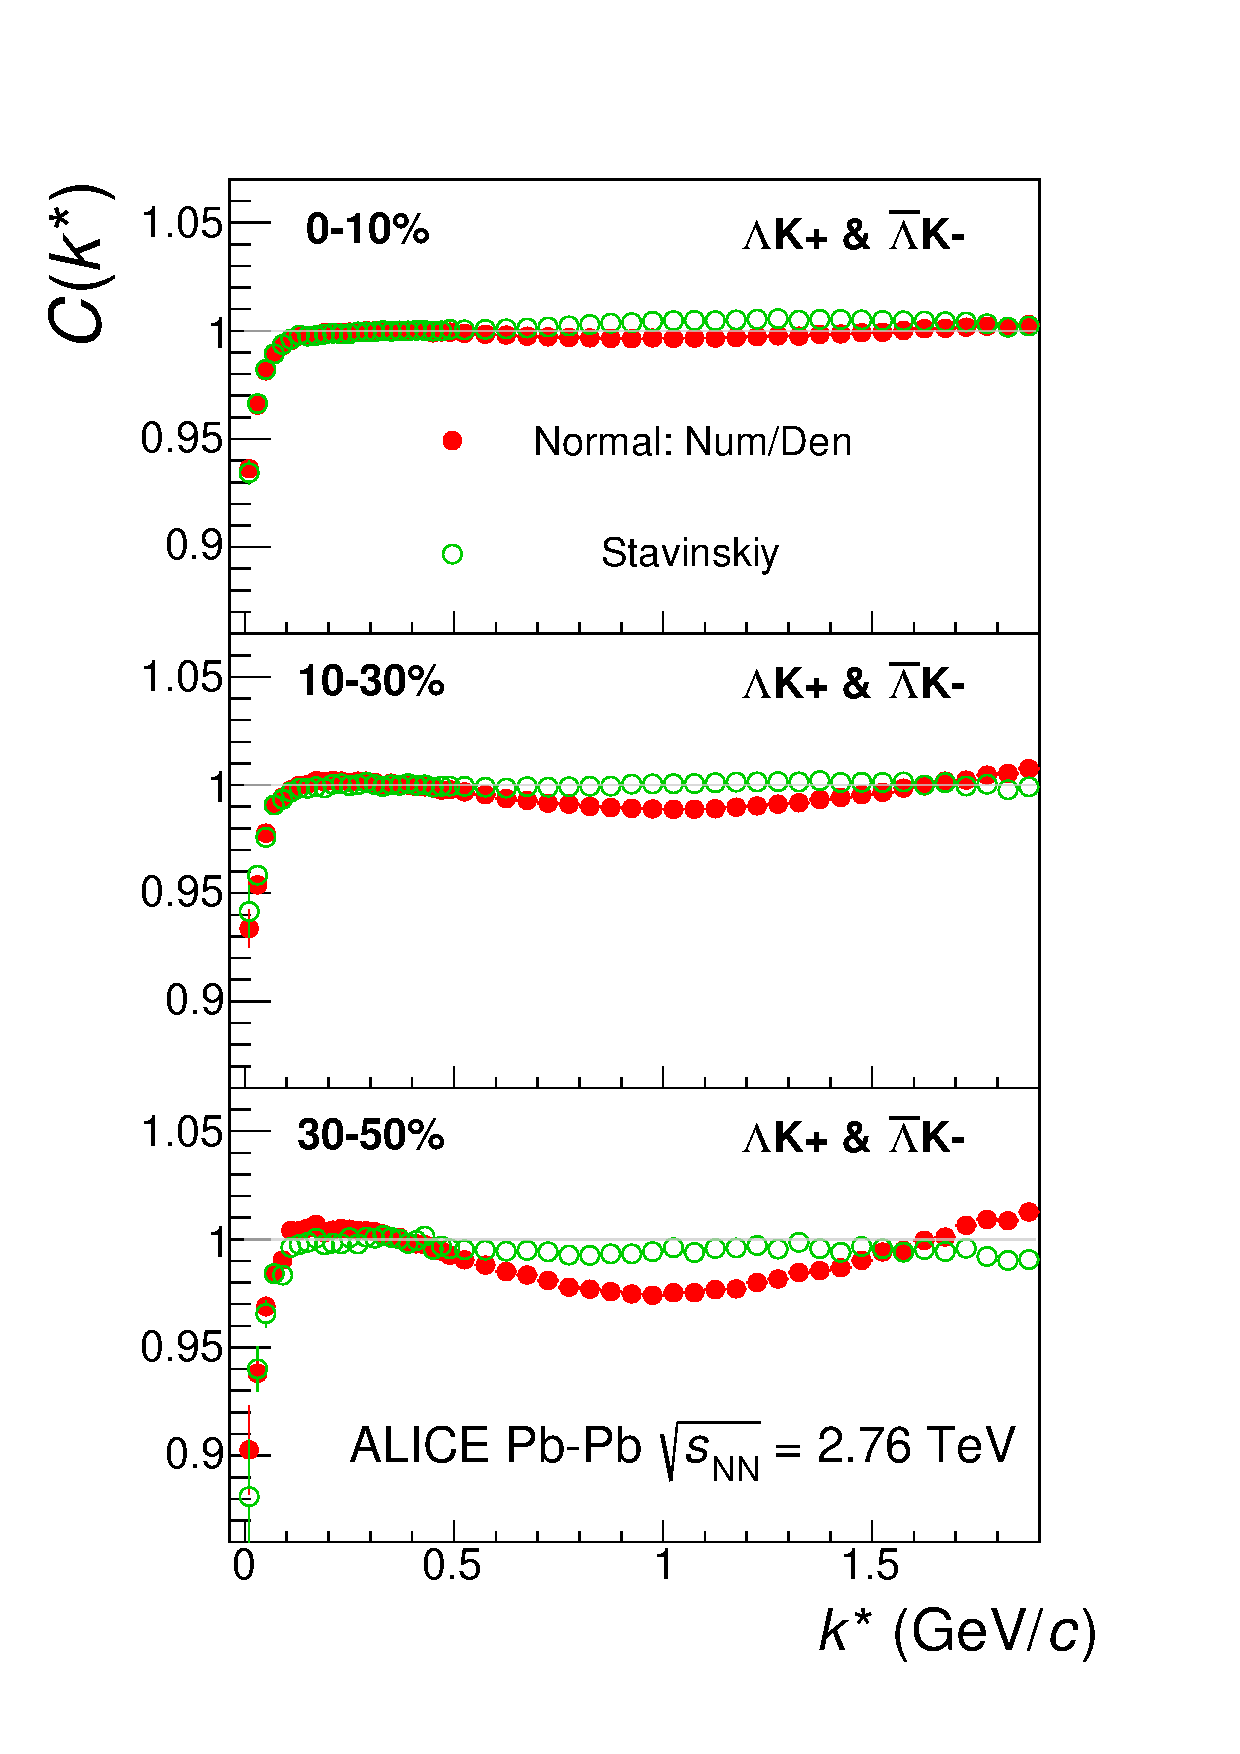
\includegraphics[width=0.667\textwidth]{/home/jesse/Analysis/FemtoAnalysis/AnalysisNotes/4_CorrelationFunctions/Figures/OnlyTwo/canKStarCfsLamKchPCombConj_20180505vs20180505StavCf_CustomRebin.pdf}
+  \caption[\LamKchP Stavinskiy Correlation Functions]
+  {
+  (Color online) \LamKchPALamKchM correlation functions built using the Stavinskiy method for 0--10\%, 10--30\%, and 30--50\% centralities.  Closed symbols represent correlations built using the normal mixed-event reference distribution, while open symbols represent correlations formed using the Stavinskiy same-event pseudo-pairs as a reference.
+  }
+  \label{fig:StavCfs_Correct_LamKchP}
+\end{figure} 
+
 
 
 
 \section{Strong and Coulomb Fitter}
 \label{App:CoulombFitter}
 
-When modeling systems which include both strong and Coulomb effects, Eq. \ref{eqn:LednickyEqn} is no longer valid, and, in fact, there is no analytical form with which to fit.
-To solve such a problem, and to fit such a system, one must develop a more fundamental model, beginning with Eq. \ref{eqn:KooninPrattEqn} and using the two-particle wave-function including both strong and Coulomb interactions \cite{Lednicky:2005tb}:
+When modeling systems which include both strong and Coulomb effects, Eq.\ \ref{eqn:LednickyEqn} is no longer valid, and, in fact, there is no analytical form with which to fit.
+To solve such a problem, and to fit such a system, one must develop a more fundamental model, beginning with Eq.\ \ref{eqn:KooninPrattEqn} and using the two-particle wave-function including both strong and Coulomb interactions \cite{Lednicky:2005tb}:
 
 \begin{equation}
  \Psi_{\mathbf{k^{*}}}(\mathbf{r^{*}}) = e^{i\delta_{c}}\sqrt{A_{c}(\eta)}[e^{i\mathbf{k^{*}} \cdot \mathbf{r^{*}}}F(-i\eta,1,i\xi) + f_{c}(k^{*})\frac{\tilde{G}(\rho,\eta)}{r^{*}}]
@@ -1223,32 +1268,24 @@
 
 where $\rho = k^{*}r^{*}$, $\eta = (k^{*}a_{c})^{-1}$, $\xi = \mathbf{k^{*}} \cdot \mathbf{r^{*}} + k^{*}r^{*} \equiv \rho(1+\cos\theta^{*})$, and $a_{c} = (\mu z_{1}z_{2}e^{2})^{-1}$ is the two-particle Bohr radius (including the sign of the interaction).  
 $\delta_{c}$ is the Coulomb s-wave phase shift, $A_{c}(\eta)$ is the Coulomb penetration factor, $\tilde{G} = \sqrt{A_{c}}(G_{0} + iF_{0})$ is a combination of the regular ($F_{0}$) and singular ($G_{0}$) s-wave Coulomb functions.  
-$f_{c}(k^{*})$ is the s-wave scattering amplitude:
-
+$f_{c}(k^{*})$ is the s-wave scattering amplitude
 \begin{equation}
- f_{c}(k^{*}) = [\frac{1}{f_{0}} + \frac{1}{2}d_{0}k^{*2} - \frac{2}{a_{c}}h(\eta) - ik^{*}A_{c}(\eta)]^{-1}
+ f_{c}(k^{*}) = \left[\frac{1}{f_{0}} + \frac{1}{2}d_{0}k^{*2} - \frac{2}{a_{c}}h(\eta) - ik^{*}A_{c}(\eta)\right]^{-1}
 \label{eqn:CoulombScattAmp}
 \end{equation}
-
-where, the ``h-function", $h(\eta$), is expressed through the digamma function, $\psi(z)$ = $\Gamma'(z)/\Gamma(z)$ as:
-
+where, the ``h-function", $h(\eta$), is expressed through the digamma function, $\psi(z)$ = $\Gamma'(z)/\Gamma(z)$ as
 \begin{equation}
  h(\eta) = 0.5[\psi(i\eta) + \psi(-i\eta) - \ln(\eta^{2})]
 \label{eqn:LednickyHFunction}
 \end{equation} 
-
 In this case, the $\lambda$ parameter may be included as: 
-
 \begin{equation}
  C(\mathbf{k^{*}}) = (1 - \lambda) + \lambda\int S(\mathbf{r^{*}})|\Psi^{S}_{\mathbf{k^{*}}}(\mathbf{r^{*}})|^{2}d^{3}\mathbf{r^{*}}
 \label{eqn:GenCfEqnwLambda}
 \end{equation}
-
 To build a fit function for a system including both strong and Coulomb interactions two related options were considered. 
-The first option was to numerically integrate Eq.\ref{eqn:KooninPrattEqn}.  
-The second option was to simulate a large sample of particle pairs, calculate the wave function describing the interaction, and average to obtain the integral in Eq.\ref{eqn:KooninPrattEqn}. 
-In either case, the solution would involve some very complicated mathematical functions, as can be seen in Eqs. \ref{eqn:CoulombWaveFcn} to \ref{eqn:LednickyHFunction}.
-Having no experience with either of these options, we elected the latter of simulating pairs. 
+The first option was to numerically integrate Eq.\ \ref{eqn:KooninPrattEqn}.  
+The second option was to simulate a large sample of particle pairs, calculate the wave function describing the interaction, and average to obtain the integral in Eq.\ \ref{eqn:KooninPrattEqn}. 
 
 %\clearpage
 
@@ -1259,7 +1296,7 @@
 \label{app:SphericalHarmonics}
 
 
-In Fig. \ref{fig:LamKchP_ReC00C11_0010} results are shown for the $C_{00}$ and $\Re C_{11}$ components from the spherical decomposition of our \LamKchP system in the 0--10\% centrality bin.
+In Fig.\ \ref{fig:LamKchP_ReC00C11_0010} results are shown for the $C_{00}$ and $\Re C_{11}$ components from the spherical decomposition of our \LamKchP system in the 0--10\% centrality bin.
 As seen in the figure, the $C_{00}$ signal is similar to that observed in the one-dimensional study.
 The $\Re C_{11}$ component shows a clear deviation from zero, and the negative value signifies that the \Lam particles are, on average, emitted further out and/or earlier than the K mesons.
 
@@ -1278,26 +1315,26 @@
 \section{Relative Emission Shifts with THERMINATOR 2}
 \label{App:THERM}
 
-Fig. \ref{fig:LamKchP_StdThermSources} shows results from the THERMINATOR 2 event generator for an impact parameter of b = 2 fm.
-As THERMINATOR does not include any final state effects, the femtoscopic correlation was introduced by assuming a set of scattering parameters ($\Re f_{0}, \Im f_{0}, d_{0}$) = ($-1.16, 0.51, 1.08$) and weighting the signal distribution (numerator pairs) with the modulus squared of the two-particle wave function, $|\Psi|^{2}$.
-
-The top left of Fig. \ref{fig:LamKchP_StdThermSources_Spatial} shows a fit to the one-dimensional correlation function from THERMINATOR 2.
+Fig.\ \ref{fig:LamKchP_StdThermSources} shows results from the THERMINATOR 2 event generator for an impact parameter of $b = 2$ fm.
+As THERMINATOR 2 does not include any final state effects, the femtoscopic correlation was introduced by assuming a set of scattering parameters ($\Re f_{0}, \Im f_{0}, d_{0}$) = ($-1.16, 0.51, 1.08$) and weighting the signal distribution (numerator pairs) with the modulus squared of the two-particle wave function, $|\Psi|^{2}$.
+
+The top left of Fig.\ \ref{fig:LamKchP_StdThermSources_Spatial} shows a fit to the one-dimensional correlation function from THERMINATOR 2.
 The scattering parameters are known precisely here, as they served as the weights used in the simulation, and are kept constant in the fit.
 Only the extracted one-dimensional source size is of interest here, so the $\lambda$ parameter is also fixed at unity.
-The other three plots in Fig. \ref{fig:LamKchP_StdThermSources_Spatial} show the source distribution in the out (top right), side (bottom left), and long (bottom right) directions (all in the PRF).
+The other three plots in Fig.\ \ref{fig:LamKchP_StdThermSources_Spatial} show the source distribution in the out (top right), side (bottom left), and long (bottom right) directions (all in the PRF).
 The source distributions have all been fitted with a Gaussian form, the result of which is printed within the respective plot.
 One immediately sees a significant shift in the out direction, $\mu_{\mathrm{out}} \approx$ 4 fm, and negligible shift in the other two directions, $\mu_{\mathrm{side}} \approx \mu_{\mathrm{long}} \approx$ 0 fm.
 The figure demonstrates that, within the THERMINATOR 2 model, the \Lam is, on average, emitted further out that its K partner.
-Finally, Fig. \ref{fig:LamKchP_StdThermSources_Temporal} shows the distribution of the relative time of emittance, again in the PRF.
+Finally, Fig.\ \ref{fig:LamKchP_StdThermSources_Temporal} shows the distribution of the relative time of emittance, again in the PRF.
 The figure shows that the \Lam is, on average, emitted earlier than its K partner. 
 
 This section concludes with a brief look at how a spatial separation of the single particle sources affects the radii extracted from a femtoscopic analysis.
 To achieve this, THERMINATOR 2 is used in a similar fashion as described above, but with one important difference.
 Instead of taking the source information from THERMINATOR 2, the source is drawn from a pre-determined Gaussian distribution.
 In all cases, $R_{\mathrm{out}} = R_{\mathrm{side}} = R_{\mathrm{long}}$ = 5 fm, and $\mu_{\mathrm{side}} = \mu_{\mathrm{long}}$ = 0 fm.
-In Figure \ref{fig:LamKchP_ThermSources_VaryMuOut}, results are shown for the case of $\mu_{out}$ = 1 fm, $\mu_{out}$ = 3 fm, and $\mu_{out}$ = 6 fm.
+In Figure \ref{fig:LamKchP_ThermSources_VaryMuOut}, results are shown for the case of $\mu_{\mathrm{out}}$ = 1 fm, $\mu_{\mathrm{out}}$ = 3 fm, and $\mu_{\mathrm{out}}$ = 6 fm.
 In this figure, the side and long distributions are not shown, as they are simple Gaussians of width 5 fm centered about the origin.
-The figure demonstrates that as the separation $\mu_{out}$ increases, so do the extracted femtoscopic radii.
+The figure demonstrates that as the separation $\mu_{\mathrm{out}}$ increases, so do the extracted femtoscopic radii.
 
 \begin{figure}[h!]
   \centering
@@ -1310,7 +1347,10 @@
     \label{fig:LamKchP_StdThermSources_Temporal}
     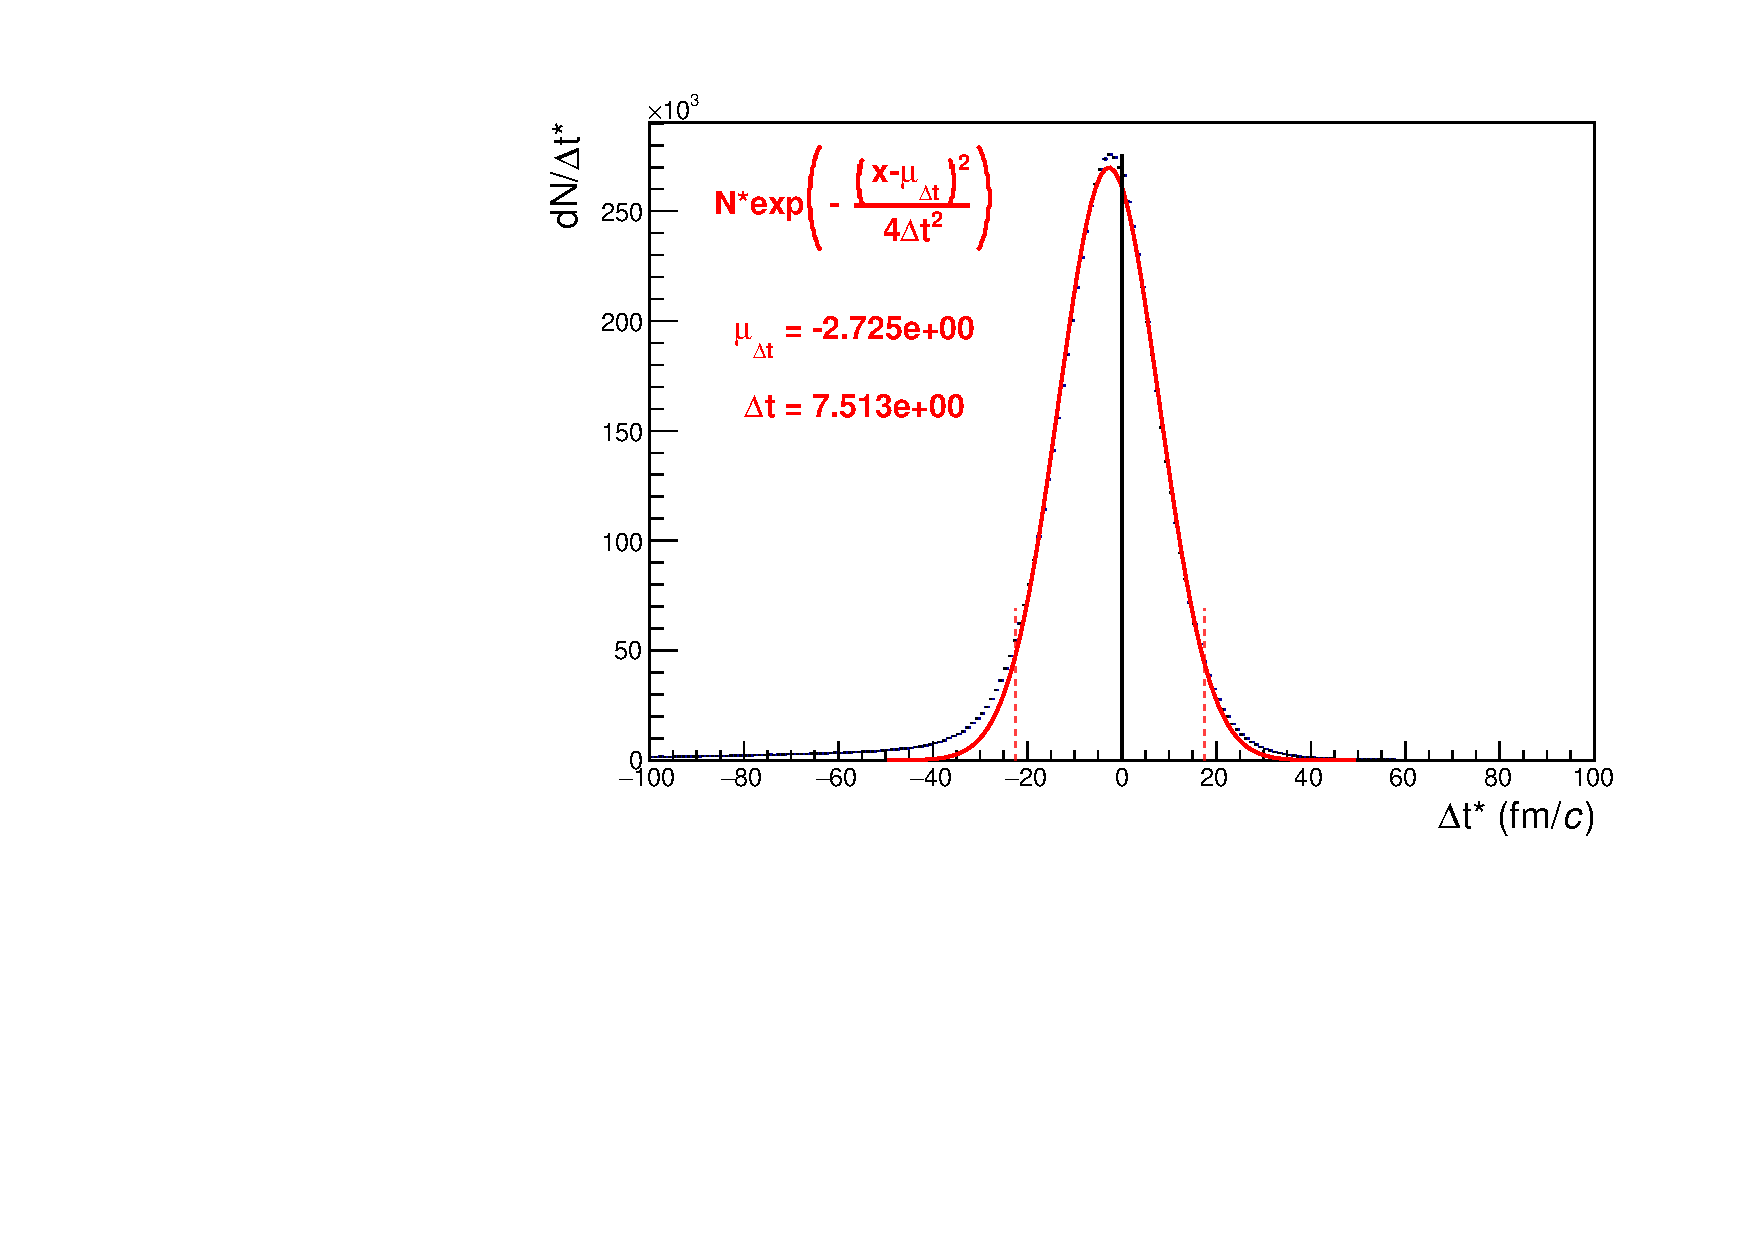
\includegraphics[width=0.60\linewidth]{/home/jesse/Analysis/FemtoAnalysis/AnalysisNotes/7_ResultsAndDiscussion/7.1_ResultsLamK/7.1.2_ResultsLamK_DiscussionOfmTScaling/ThermPlots/LamKchP/CanDeltaT_Full_LamKchP_FromFileCorrelationFunctions_wOtherPairs_BuildCfYlm.pdf}}  
   %%----overall caption----
-  \caption[Extracted Radius and Pair Sources from THERMINATOR 2]{Extracted radius when performing a simple fit on simulation from THERMINATOR 2, along with the spatio-temporal characteristics generated by the simulation.}
+  \caption[Extracted Radius and Pair Sources from THERMINATOR 2]
+  {
+  (Color online) Extracted radius when performing a simple fit on simulation from THERMINATOR 2, along with the spatio-temporal characteristics generated by the simulation.
+  }
   \label{fig:LamKchP_StdThermSources}
 \end{figure}
 
@@ -1321,11 +1361,11 @@
   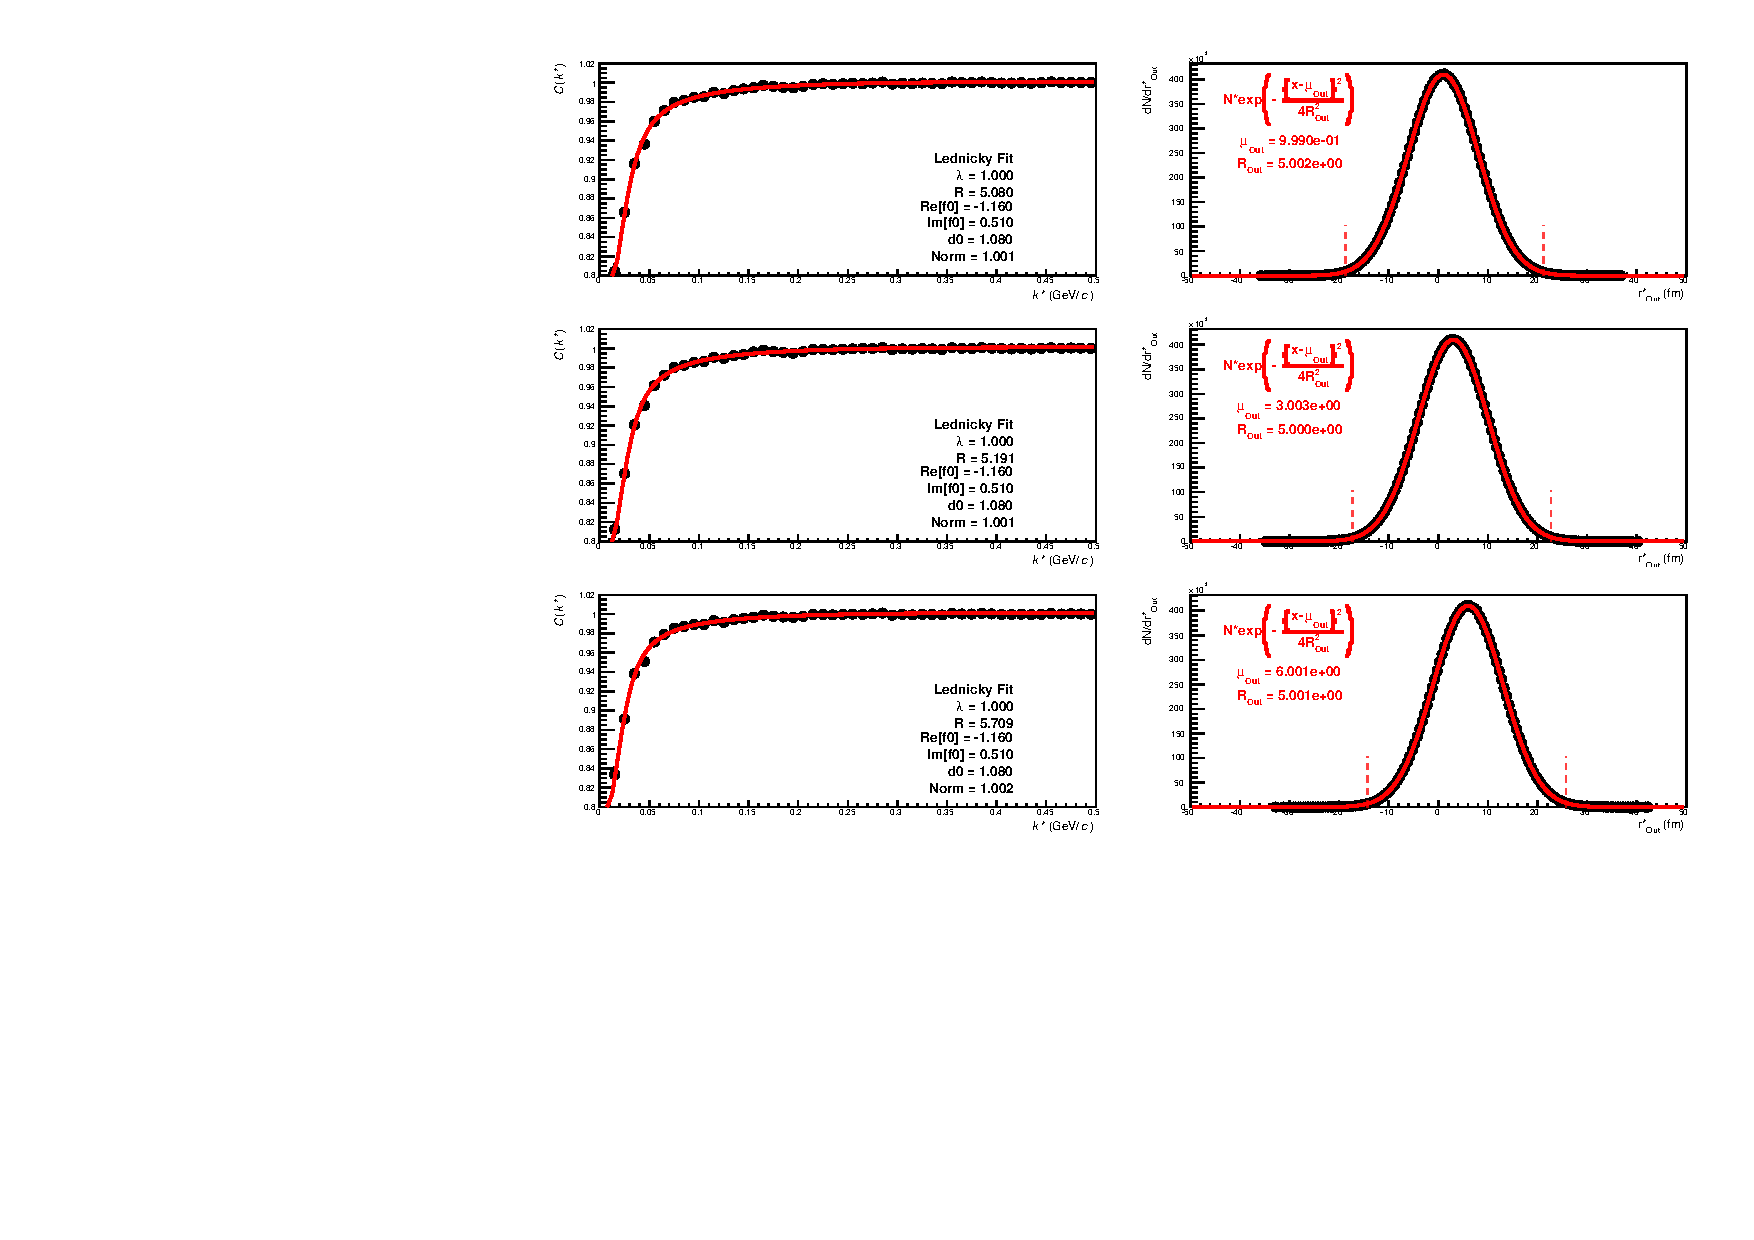
\includegraphics[width=\textwidth]{/home/jesse/Analysis/FemtoAnalysis/AnalysisNotes/7_ResultsAndDiscussion/7.1_ResultsLamK/7.1.2_ResultsLamK_DiscussionOfmTScaling/ThermPlots/LamKchP/CanCompMus_Full_LamKchP_3dHistPairSource3d_oslLamKchP.pdf}
   \caption[Varying $\mu_{\mathrm{Out}}$ with THERMINATOR 2]
   {
-  Probing the effect of varying the source shift in the outward direction, $\mu_{\mathrm{Out}}$, within the THERMINATOR 2 framework.  
-  To achieve this, particle pairs are formed from the simulation, but with altered spatial characteristics achieved by drawing the out, side, and long components from pre-determined Gaussian distributions.  
+  (Color online) Probing the effect of varying the source shift in the outward direction, $\mu_{\mathrm{out}}$, within the THERMINATOR 2 framework.  
+  To achieve this, particle pairs are formed from the simulation, but with altered spatial characteristics achieved by drawing the out, side, and long components from predetermined Gaussian distributions.  
   The plots on the left show fits resulting from the sources (in the out direction) shown on the right.  
   The sources in the side and long directions are not shown, and are both Gaussians of width 5 fm centered at the origin for all cases.  
-  Moving from top to bottom, $\mu_{\mathrm{Out}}$ increase from 0 to 6 fm, the effect of which clearly increases the effective radius extracted in the fit.
+  Moving from top to bottom, $\mu_{\mathrm{out}}$ increase from 0 to 6 fm, the effect of which clearly increases the effective radius extracted in the fit.
   }
   \label{fig:LamKchP_ThermSources_VaryMuOut}
 \end{figure}

